\documentclass[12pt]{report}
\author{Nicholas Berezny}
\title{Thesis Outline}
\usepackage{cite}
\usepackage{fullpage}
\usepackage{gensymb}
\renewcommand{\baselinestretch}{1.5} 

\usepackage{amsmath}
\usepackage{graphicx}
\graphicspath{ {pics/} }
\usepackage{svg}
\usepackage{hyperref}

\usepackage{multirow}
\usepackage{adjustbox}
\usepackage{color, colortbl}
\usepackage{xcolor}
\usepackage{booktabs}

\begin{document}
\maketitle
\newpage

\chapter*{Abstract}
\chapter*{Acknowledgements}

\tableofcontents
\listoffigures
\listoftables

\chapter{Literature Review and Preliminary Research}


\section{Stroke and Rehabilitation}

Stroke is a cerebrovascular disease which effects approximately 62,000 Canadians and 795,000 Americans each year \cite{Benjamin2018,Hebert2016}. It is among the leading casuses of adult disability \cite{Ewart2003}, with some form of motor impairment effecting 80\% of patients, which can result in limited mobility and muscle control \cite{Langhorne2009}. Ischaemic stroke is the most common form of stroke, accounting for around 80\% of all cases \cite{Rey2008}. It is caused by blood vessel occlusion, either directly in the brain (thrombotic), or due to the migration of a clot formed somewhere else in the body (embolic). The subsequent lack of oxygen causes the death of brain tissue and neurological deficits \cite{Prabhakaran2015}, which manifest as functional impairments in activities associated with the affected brain region. Stroke complications can include hemiparesis (weakness on one side of the body), muscle spacitity, loss of motor control, and loss of dexterity, all of which can effect the patient's ability to perform activities of daily living (ADL's) and compromise their autonomy. In addition to medical intervention in the form of pharmaceuticals and surgery, the stroke patient may require rehabilitation to reduce functional impairment \cite{Stroke}. It is imperative to administer treatment during the acute phase of the stroke (\textit{i.e.} within days of the stroke) \cite{Prabhakaran2015}.

%----
%Approximately 62,000 Canadians suffer from stroke every year, with over 10\% of victims requiring in-patient rehabilitation \cite{Benjamin2018,Hebert2016}. It is among the leading casuses of adult disability \cite{Ewart2003}. Motor impairment effects around 80\% of patients, which can result in limited mobilited and muscle control \cite{Langhorne2009}. The scale of stroke care and rehabilitation is significant, with ... Improving stroke rehabilitation would benefit the stroke victims by improving their recovery and thus their quality of life, and would also have significant economic benefits, with one study estimating up to \$682 million dollars annually in Canada alone, due to savings due to earlier discharges, as well as increased productivity of the stroke patients post-treatment \cite{Krueger2012}. 
%----

%Ischaemic stroke is the most common form of stroke, accounting for around 80\% of all cases \cite{Rey2008}. It is caused by blood vessel occlusion, either directly in the brain (thrombotic), or due to the migration of a clot formed somewhere else in the body (embolic). The subsequent lack of oxygen in the affected area of the brain causes the death of brain tissue and neurological deficits \cite{Prabhakaran2015}, which manifest as functional impairments in the patient in activities associated with the affected brain region. Stroke complications can include hemiparesis (weakness on one side of the body), muscle spacitity, loss of motor control, loss of dexterity, etc... In addition to medical intervention in the form of pharmaceuticals and surgery, the stroke patient may require rehabilitation to reduce functional impairment and, ideally, to recover full autonomy \cite{Stroke}.

Older treatment techniques relied on compensatory measures to assist stroke patients in regaining autonomy \cite{Dobkin2004}. Using rehabilitation to restore autonomy began to be emphasized once the concept of neural plasticity became more widely accepted. Neural plasticity is the process by which new connections are formed in the central nervous system in response to experience or activities performed by the subject \cite{Warraich2010}. When a stroke patient repetitively performs motor tasks, new neural connections in the brain are formed which take on the role of the regions of the brain which were damaged. This allows the patient to re-learn tasks such as walking by going through intensive rehabilitation. 

%Rehabilitation of lost abilities began to be emphasized over compensatory measures due to the discovery of neural plasticity and its role in the process of learning new tasks. The basis of this neural plasticity is the formation of new neural connection in the brain in response to a repeated movement or activity. In the case of stroke, this allows new neurons to take on the role of damaged regions in the brain, allowing the patient to effectively re-learn tasks such as walking. 
	\begin{figure*}[h] 
		\centering
		
\includegraphics[width=0.6\linewidth]{leg_lift}
		\caption{Example of the leg lift exercise}
		\label{fig:leg_lift}
	\end{figure*}
	
		\begin{figure*}[h] 
		\centering
		
\includegraphics[width=0.6\linewidth]{knee_extension}
		\caption{Example of the knee extension/flexion exercise}
		\label{fig:knee_ext}
	\end{figure*}

Stroke rehabilitation encompasses a broad range of therapeutic activities, typically carried out by occupational- and physiotherapists. Physiotherapists (PT's) tend to focus on gross motor movements in the upper and lower limbs, while occupational therapists (OT's) focus on fine motor control, dexterity, and specific ADL's. These two goals are inextricably linked, and so both PT's and OT's form a team which works together to improve patient outcomes. The rehabilitation carried out by both OT's and PT's involves the repetition of a target movement or task. Depending on the abilities of the patient, the therapist may provide support or assistance. For example, lower-limb rehabilitation begins with simple legs movement performed in bed, such as leg lifts (Fig. \ref{fig:leg_lift}), knee flexion/extension (Fig. \ref{fig:knee_ext}), hip abductions, \textit{etc}. The therapist can either assist the patients leg through the movement, or allow patients to perform the movement on their own, or even provide light resistance if the patient is more advanced. Next, the patient will practice sitting upright, going from sit to stand, and  practice bearing weight and balancing while standing. Eventually the patients will be ready for more complex tasks with assistance from the therapist, including walking, heel strike, and stair climbing. The patient may advance to the point where they can walk without therapist assistance, using either parallel bars, a walker, or potentially without any assistance. The stages of lower-limb rehabilitation are summarized below:


	\begin{figure*}[h] 
		\centering
		\includegraphics[width=\linewidth]{Traditional_therapy}
		\caption{The stages of traditional stroke rehabilitation}
		\label{fig:stages}
	\end{figure*}


\subsection{Rehabilitation Guidelines}

Canadian stroke best practices recommend that therapy involves the repetition of intensive, task-specific activities in a complex and stimulating environment \cite{Hebert2016}. Lower-limb rehabilitation should be goal-orientated towards selected tasks such as walking and sit-to-stand. Robotics, virtual reality, and biofeedback are all mentioned as potential adjuncts, but are not recommended to replace traditional therapy. It is also recommended that patient's should receive rehabilitation as early as possible once they are deemed medically ready. Early mobilisation is recommended (within 24-48 hours of stroke, \cite{Casaubon2016}, but not before 24 hours due to findings that this actually reduces functional outcomes, \cite{AVERTTrialCollaborationgroup2015}). Active participation on the part of the patient is also imperative [4], as it has been found that this facilitates neural plasticity. This requires that the patient be engaged in the therapy (hence the need for stimulating environments), and also requires the therapist to ensures that the rehabilitation is not passive.

Therapy dosage also has an effect on functional outcomes. For example, one study found positive correlation between time scheduled for therapy and most functional outcomes \cite{Lohse2014}. Another study sought to determine if current doses of rehabilitation are enough to trigger functional improvements by comparing with animal models \cite{Lang2009}, and found that the amount of rehabilitation they observed was inadequate. Another study found that stroke inpatients spend on average 13\% engaged in physical activities and 5.2\% of their time with a therapist \cite{Bernhardt2004}. Other studies confirm that stroke patients spend a significant amount of time in or sitting near their bed \cite{King2011}. These results indicate the importance of scheduling time specifically for rehabilitation for stroke inpatients. 

	\begin{figure*}[h] 
		\centering
		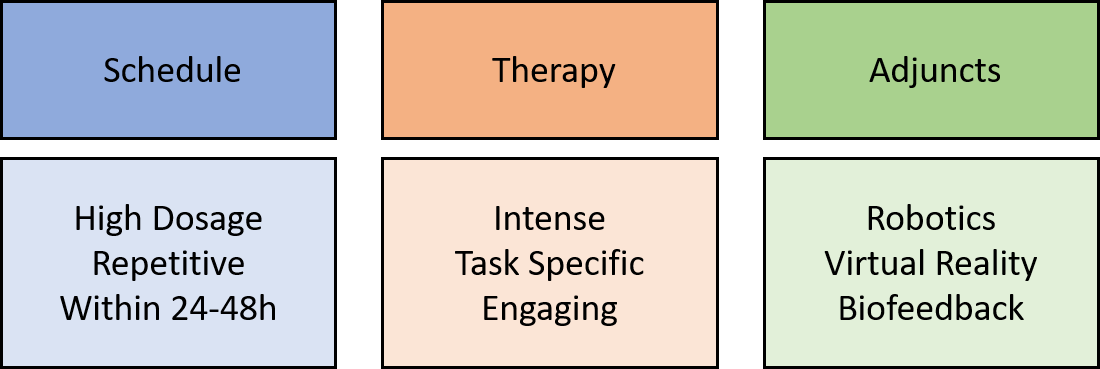
\includegraphics[width=0.75\linewidth]{guidelines}
		\caption{Stroke Rehabilitation Guidelines}
		\label{fig:guidelines}
	\end{figure*}

Other factors may restrict the PT's and OT's ability to accomplish the recommended best practices. The intensity and duration of the therapy is limited both by the endurance of the patient and of the therapist, as the physical burden of manually assisting the patient may be high \cite{Colombo}. Furthermore, providing task-specific and stimulating therapy is difficult, particularly when doing bed-bound exercises which are not easily relatable to ADL's. One study found that therapy dosage may be affected by understaffed units, resulting in less rehabilitation time with therapists \cite{Mchugh2013}. There is an opportunity to introduce new methods or technologies to assist therapists in delivering more rehabilitation.

A stroke patient's progress is monitored through tests, surveys, and measures. The Berg Balance Scale, Barthel Index, Stroke Rehabilitation Assesment of Movement (STREAM), and the Timed Up and Go (TUG), are all examples of measures used to track lower-limb rehabilitation progress \cite{Salbach2001}. The Berg Balance scale is used to describe the patient's ability to remain balanced during different tasks. The Barthel index is used to rate the patient's ability to perform a number of ADL's, such as dressing and grooming. Rehabilitation progress is directly monitored in STREAM, which takes into account mobility, range of motion, and coordination. The TUG score measures the time taken to stand up out of a chair, walk 3m, return to the chair, and sit down again. This measures mobility, balance, and also fall risk. 

%-----
%Guidelines stipulated in \cite{Hebert2016} express the need for prompt lower-limb rehabilitation, beginning ideally within days of the stroke. This is denoted the ``acute'' phase, as opposed to the ``chronic'' phase which refers to longer-term rehabilitation. The importance of acute stroke rehabilitation has been emphasized in the above guidelines and others like it as a way to improve patient outcomes. This is attributed in part to the brain's greater receptivity to changes through neural plasticity, a mechanism triggered through rehabilitation. However, starting therapy earlier may be more difficult, given that the complications are generally more pronounced. Guidelines also recommend that therapy is intensive, task-specific, and engaging \cite{Hebert2016}.  The intensity and duration of therapy may be limited by the endurance of the patient, as well as the physical burden that manually assistance places on the therapist. The frequency of therapy may also be limited by the busy schedules of PT's and OT's. 



 %Providing physical support and assistance to patient's can be burdensome for the therapist, especially when transferring patients out of bed and standing them up. The repetitive nature of rehabilitation can also be physically demanding. 


%The rehabilitation carried out by both OT's and PT's involves the repetition of a target movement or task. Depending on the abilities of the patient, the therapist may provide support or assistance. For example, typical lower-limb rehabilitation begins with simple legs movement performed in bed, such as knee flexion/extension, leg lifts, hip abductions, \textit{etc}. The therapist can either assist the patients leg through the movement, or allow patients to perform the movement on their own, or even provide light resistance if the patient is more advanced. Providing physical support and assistance to patient's can be burdensome for the therapist, especially when transferring patients out of bed and standing them up. The repetitive nature of rehabilitation can also be physically demanding. 

%A stroke patient's progress is monitored through tests, surveys, and measures...

%Inpatient's at the hospital may be discharged without having fully recovered from their impairments. They may seek outpatient clinics for further, chronic stroke rehabilitation. Many never fully recover the ability to perform all of their necessary ADL's (ref). This fact, coupled with the increasing rates of stroke, has spurred a variety of active research into improvements to current stroke intervention, and novel ways of administering rehabilitation. 

%% OLD 
%It is recommended that patients receive three hours a day of therapy, with more therapy generally leading to better outcomes. Exercises should be task-specific, meaningful, and related to activities of daily living. Giving the patient chances to repeat the exercises (under supervision) is also recommended.  The guidelines also explicitly mention both robotic devices and virtual reality training as potential tools for rehabilitation, although they should be used in addition to traditional therapy and not as replacements.  


\section{Robotic Rehabilitation}

	Rehabilitation robots have been introduced to improve the stroke rehabilitation process by automating the physical assistance usually supplied by therapists. Rehabilitation requires the repetition of a precise motion, a task well-suited to robotics. Over the past few decades, a variety of robotic platforms have been developed for many different therapeutic activities, from lower-limb gait training to fine motor skills in the hand. There are many other potential benefits for using robotics for rehabilitation, including the following.
\begin{itemize}
	\item \textbf{Relieving Physical Burden}: Using robots to provide the physical support and assistance required for stroke therapy will relieve the physical burden from therapists, removing the chance of injury or fatigue.
	\item \textbf{Increased Intensity and Duration}: Both the intensity and duration of a therapy session may be limited when relying on a therapist to provide physical assistance. With a robot, duration and intensity would only be limited by the endurance of the patient. 
	\item \textbf{Increased Dosage}: Robots could also increase the amount of rehabilitation given to patients. For example, a single therapist could supervise several patient's each using a robotic device, therefore increasing the number of patients a therapist can manage, thereby increasing the dosage each patient receives.
	\item \textbf{Providing Performance Measures}: Robots record a number of metrics not available when using traditional therapy, such as velocity, force, trajectory error, and effort. Tracking these measures could allow the therapist to better administrate therapy and track patient improvement. 
	\item \textbf{Virtual Environments}: Patient engagement could be increased by incorporating virtual reality, games, and other forms of visual feedback. The robot would serve as the control input to the environment. The relevancy of the therapy could also be improved by simulating ADL's. Finally, haptic feedback could further immerse the patient in the virtual environment by rendering virtual forces to the patient (see section \ref{Sec:VR}).
\end{itemize}
	

	Rehabilitation robots can be broadly categorized as targeting the lower-limb or the upper-limb. Upper-limb robots tend to be lighter weight since they encounter much smaller loads, while lower-limb devices are heavier as they need to support either the weight of the leg or of the entire body. Lower-limb robots can be further categorized as either targeting standing activities such as treadmill walking, or lying/sitting activities \cite{Calabro2016}. A final subdivision exists between endplate based devices and exoskeletal devices (Fig. \ref{fig:end_exo}). Endplate-based devices interact with the patient at a single point, usually the end of the limb (the hand or foot), and only apply forces through this point. Exoskeletal devices attach to the user at multiple points, offering greater control over the overall motion of the limb, although they are often more restrictive, more complex, and potentially less safe \cite{Chang2013}. One study found evidence that endplate-based devices may actually yield better outcomes than exoskeletal devices, although the comparison was done via meta-analysis of many different studies with significantly different methodologies \cite{Mehrholz2012} . 
	
	
	\begin{figure*}[h] 
		\centering
		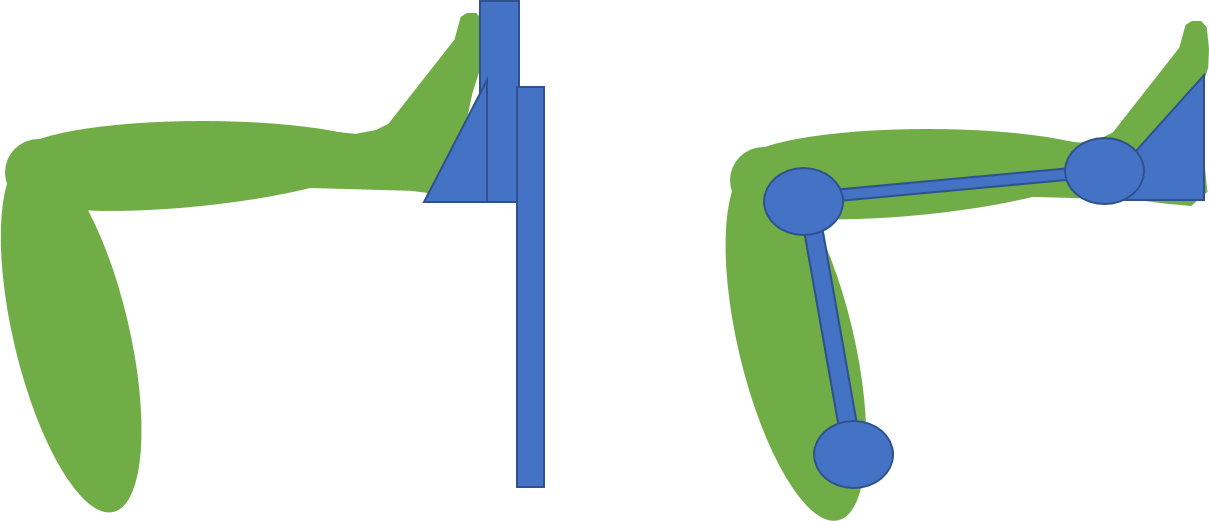
\includegraphics[width=0.8\linewidth]{endplate_exoskeleton}
		\caption{An endplate device (left) and an exoskeletal device (right)}
		\label{fig:end_exo}
	\end{figure*}

	
	Rehabilitation robots have not yet been fully endorsed by stroke best practices. For example, Canadian best practices list robots as a potential benefit, but do not recommend they replace traditional therapy \cite{Hebert2016}. This is largely due to the limited evidence for outcomes of robotic rehabilitation. Many studies are small scale case studies, and the 
few large clinical trials have found conflicting results. One study following 63 patients compared using the Lokomat (see Sec. \ref{Sec:Overground}) to conventional therapy, and found that the robot was less effective \cite{Hidler2008}. There are many challenges in studying the efficacy of robots in a clinical setting. It is unethical to replace traditional therapy with an unproven method, so typically extra therapy is added to the subject's regimen either from a robot or from a therapist (control). Since most robots are designed to replace time spent in conventional therapy, the robot must consistently be shown to be at least as effective as a therapist at delivering rehabilitation. Furthermore, since most robotic devices are substantially different, results from the study of one lower-limb robot may not apply to another robot. All of this makes ``proving'' the efficacy of a rehabilitation robot difficult. That said, there have been many different robotic devices successfully tested, with some even being available commercially. 
	
	
	\subsection{Robots for Overground Walking} \label{Sec:Overground}

	One of the most important activities for lower-limb rehabilitation is gait training, wherein the patient walks with assistance from the therapist. Rehabilitation robots were introduced to provide this assistance by attaching to the patient's leg and guiding them through the correct gait trajectories. This can be accomplished bv an exoskeletal orthosis attached around the knee joint, or by and endplate device which supports and guides the feet. 
	
	%The Lokomat, ALEX, LOPES, and ReoAmbulator are examples exoskeletal gait trainers. 
	
	
	%Each comprise of a powered exoskeleton which can assist the leg through gait trajectories. They all work in conjunction with body-weight supported treadmill training (BWSTT), using a harness to support the patient and a treadmill for walking. The Lokomat and LOPES use impedance control to deliver programmable levels of assistance to the user. ALEX uses a force-field scheme to create an ''assist-as-needed`` controller which ensures that the user contributes to the movement.
	
	The Lokomat is a powered orthosis that attaches to the patient's leg, and works in conjunction with body-weight supported treadmill training (BWSTT). It uses impedance control to provide programmable assistance to the leg through gait trajectories. The Lokomat is one of more widely researched platforms. One recent study found that the Lokomat was more effective than conventional gait therapy with regards to certain outcome measures \cite{Nam2017}, although another found that it was less effective \cite{Hidler2008}. Despite conflicting results, the Lokomat continues to show promise. It is commercially available -- 872 devices can be found worldwide according to their website (as of 2019).
			
	\begin{figure*}[h] 
		\centering
		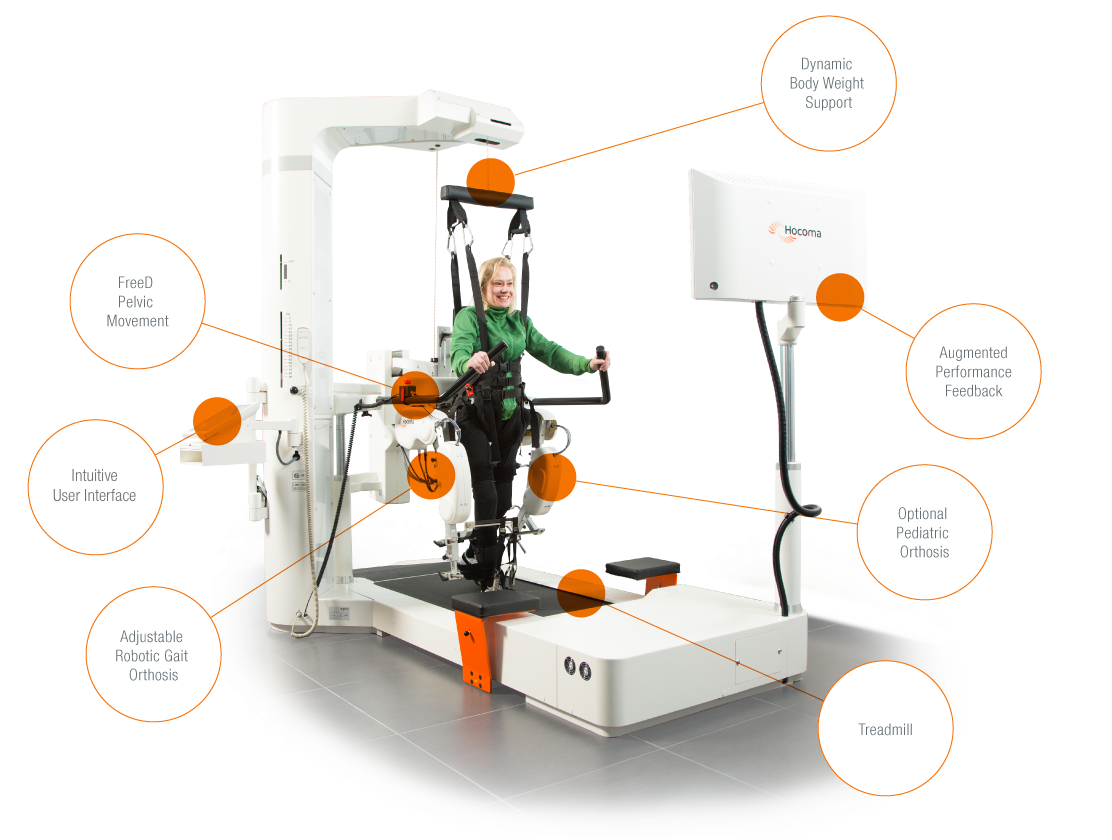
\includegraphics[width=0.75\linewidth]{Lokomat}
		\caption{The Lokomat (by Hocoma), an exoskeletal robot}
		\label{fig:Lokomat}
	\end{figure*}
	
	The ALEX \cite{Banala2007} is an exoskeletal robot used for treadmill gait training. It consists of a 8 DOF orthosis, and a harness to stabilize the user. Its controller provides assistance-as-needed using a force-field scheme, which only applies force when the user deviates from a desired trajectory. This is done by creating ``virtual walls'' at a set distance around the trajectory. They also use friction compensation to make the device backdrivable, to ensure the motion is transparent. A small study on healthy subjects showed that the force-field controller improved the user's ability to perform the trajectory. 
	
	The LOPES \cite{Veneman2007}, or the Lower Extremity Powered Exoskeleton, is gait rehabilitation robot similar to the Lokomat and the ALEX. It uses impedance control to provide modes like patient-in-charge and robot-in-charge. The device has three DOF's per leg, and also contains a pelvic support system to hold the patient up, which is itself also actuated by three linear DOFs. A small study looked at EMG data from normal treadmill walking with treadmill walking with the LOPES, and found that both produced similar data, suggesting unhindered walking is possible with the LOPES.
	
	The ReoAmbulator
	
	
	%The Haptic Walker , G-EO , and Gait Trainer  are examples of end-plate based rehabilitation robots. Both use actuated platforms under the feet to move the patient through gait trajectories, and a harness to support the patient. The Haptic Walker can perform walking simulations and more complex situations like stumbling or climbing stairs using a 3 DOF system. As can be seen in Figure \ref{fig:Hapticwalker}, the system is much larger than the exoskeletal systems. The GE-O system is similar in that it can simulate walking and stair climbing, with one study finding that electromyography (EMG) readings were similar between simulated walking with the robot and real walking \cite{Hesse2010}. 
	
	\begin{figure*}[h] 
		\centering
		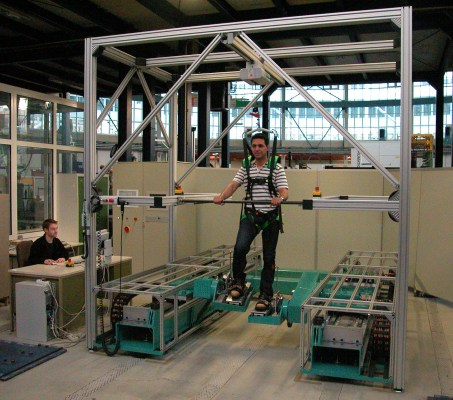
\includegraphics[width=0.75\linewidth]{Hapticwalker}
		\caption{The Hapticwalker, an endplate based robot}
		\label{fig:Hapticwalker}
	\end{figure*}
	
	The HapticWalker \cite{Schmidt2005} is an endplate-based gait trainer with two actuated platforms that can move the user's leg through the sagittal plane (Fig. \ref{fig:Hapticwalker}). The system has 3 DOF per leg, but can be extended to 6 DOF to allow for a greater range of motions. The control software is implemented in RTLinux, and includes trajectory generation and a User interface. As can be seen in Fig. \ref{fig:Hapticwalker}, the HapticWalker, along with other endplate devices targetting standing activities, tend to be much larger than and also require more power.
	
	The G-EO is a endplate-based robot designed for the repetitive practice of floor walking and stair climbing \cite{Hesse2010}. Similarly to the HapticWalker, it has two actuated platforms which can guide the patient's legs through trajectories. This robot uses position control, which does not necessarily encourage patient engagement. 
	
	%The Gait Trainer \cite{Hesse}
	
	Overground walking robots show promise for improving gait rehabilitation. However, these only target a single type of lower-limb rehabilitation. Patients must be somewhat mobile (enough to leave their beds and their rooms) to access these devices, and the complexity and setup require that a therapist be present. Hence these robots are designed to replace time spent on conventional therapy, which makes proving consistent performance difficult as was previously mentioned. 
	
	\subsection{Robots for Sitting or Bed-bound Therapy}
	
	Some types of rehabilitation are administered while the patient is sitting or reclined in bed, often for acute stroke patient's who are not yet mobile. Robots for assisting in activities while the patient sits or lies down are less common in the literature. The MotionMaker, Lambda, and ViGRR are some examples. 
	
	The MotionMaker (Fig. \ref{fig:Motionmaker}) consists of a reclinable chair and two orthoses, which attach to the leg only at the foot \cite{Schmitt2004}. It uses a regulator with force feedback to control the exercise. It is designed to be used in conjunction with functional electrical stimulation for spinal cord injury patients, but it's application extends to lower-limb rehabilitation in general. 
	
	\begin{figure*}[h] 
		\centering
		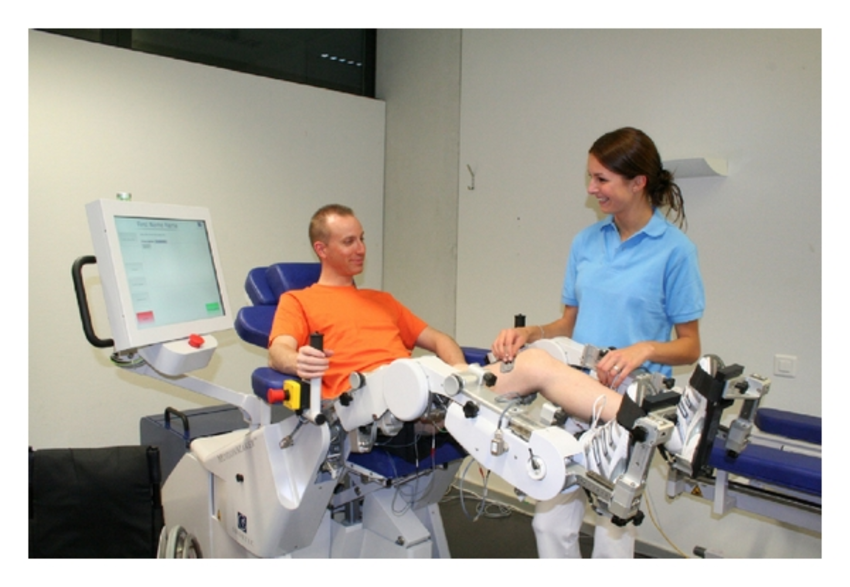
\includegraphics[width=0.75\linewidth]{Motionmaker}
		\caption{The MotionMaker}
		\label{fig:Motionmaker}
	\end{figure*}
	
	The Lambda (Fig. \ref{fig:Lambda}) is robot developed for general lower-limb rehabilitation and for fitness purposesd \cite{Bouri2009}. It uses parallel linkages with a total of 3 DOFs to achieve a variety of motions. An adjustable seat allows the user to recline as needed. Recent developments include the addition of virtual reality and games to engage the patient, enhanced feedback regarding the patients progress, and multiple types of exercises. 
	
	\begin{figure*}[t] 
		\centering
		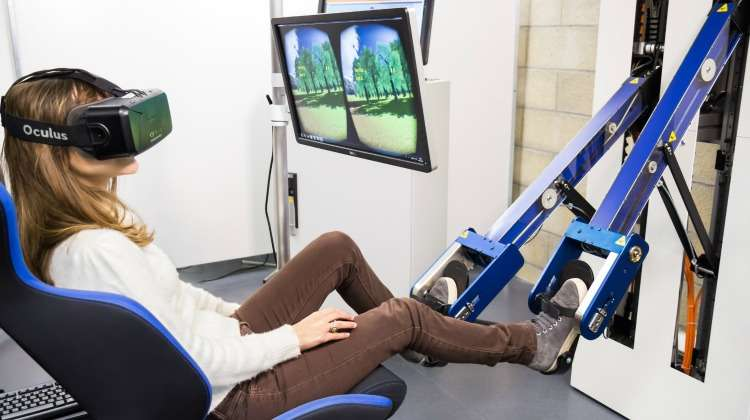
\includegraphics[width=0.75\linewidth]{Lambda}
		\caption{The Lambda}
		\label{fig:Lambda}
	\end{figure*}
	
	The Rutger's Ankle \cite{Burdea2000} is an endplate based robot used to rehabilitate the ankles. It's design is based on the Stewart platform, in that it is actuated by six linear actuators to achieve 6 DOF's. The foot is attached to the top plate, and a 6 DOF force sensor is used to measure user input. The system is coupled with a virtual environments, each which focus on a different therapeutic activity. The goals set in the virtual environments are meant to motivate patients to perform the correct rehabilitation activity. The device is designed for at home use. While initial experiments showed some patients became fatigued, or were confused by the virtual environments, the overall results were positive. 
	
	The precursor to this project is the Virtual Gait Rehabilitation Robot (ViGRR), a device developed at Carleton University's Advanced Biomechatronics and Locomotion Laboratory \cite{Chisholm2014, Chisholm2010}. It is a 4-DOF end-plate based robot which can assist a reclined patient move through trajectories in the sagittal plane. The user's foot interfaces with a footplate which is magnetically attached to the robot. The magnet can be released if triggered by safety system, including high force, high velocity, or pressing an emergency stop button. An admittance controller is used to provide assistance-as-needed, roughly in proportion to the trajectory error. These desired trajectories can include gait trajectories, linear motion, circular motion, or any other path in the sagittal plane. To increase user engagement, a virtual environment was created which can display visual feedback regarding the desired trajectory, or games such as pushing a block or brick breaker. User's can be further immersed in the virtual environment through haptic feedback. For example, when pushing on virtual wall, the robot will apply a force to the user's foot emulating the wall reaction force. 
	
	
	\begin{figure*}[t] 
		\centering
		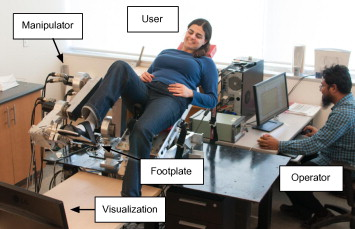
\includegraphics[width=0.75\linewidth]{Vigrr}
		\caption{ViGRR}
		\label{fig:vigrr}
	\end{figure*}	
	
	
	%The motivation to create a new device is twofold: creating a lower-powered device suitable for acute stroke rehabilitation, and a smaller and more light-weight device suitable for the hospital environment. 

	
	
	\subsection{Controls} 
	
	The type of controller used is especially important for devices interacting with a human (or any unknown environment), as it will determine the interaction behaviour and stability. The behaviour of the interaction should be optimized to ensure the patient engages in meaningful therapy driving neural plasticity and recovery. Position control through the desired trajectory is not adequate, as the robot will effectively force the limb through the motion, thus becoming a passive motion machine with no necessary engagement from the patient. Neural plasticity requires engagement, \textit{i.e.} the patient needs to contribute to some extent to the movement of their limbs. Therefore, rehabilitation robotics should only give some assistance to the patient, instead of leading the motion. 
	
	Three popular control laws for rehabilitation robotics are listed in \cite{Meng2015}:
	
\begin{itemize}

	\item \textbf{Impedance and admittance} control were introduced by Hogan in \cite{Hogan1985}, and have been the foundation of most interaction controllers since. These controllers determine the dynamic interaction between robot and environment instead of regulating position or force. In this way, an impedance controller can be used to give a programmable amount of assistance to the user through a trajectory, which can be varied by changing the parameters so that an optimal amount of assistance can be obtained for each individual. The desired impedance or admittance is defined in terms of a mass-spring-damper system. Therefore, changing the spring gain will change the level of assistance. The damper gain can be used to resist motion if the patient is more advanced or if strength training is the goal. This control scheme is explained in detail in Sec. \ref{Sec:imp}.
	
	\item \textbf{EMG-based} control uses electromyography (EMG) to measure muscle activity in the patient. The robot then only provides assistance when the intent to move is detected (\textit{i.e.} the patient flexes their muscle). This ensure that the patient is actively engaged in the therapy. 
	
	\item \textbf{Adaptive} control here refers to a controls which changes its behaviour over time based on some predefined law. For example, the amount of assistance supplied by an admittance controller can be changed based on patient performance. Some robots use information from movements in the patient's healthy limb to calculate the optimal control path for the affected limb. Others use assist-as-needed control schemes to only provide assistance when the patient requires it. Artificial Neural Networks have been used to determine when the assistance is needed in robots such as the ALEX and LOPES.
	
\end{itemize}
		
	\subsection{Virtual Environments} \label{Sec:VR}
	
	Virtual environments or virtual reality refer to digitally created simulations or visualizations, typically displayed through headsets or on computer monitors. It combines visuals, auditory stimulation, and haptic feedback to create an immersive experience. Virtual reality has been introduced into rehabilitation for two primary reasons \cite{Laver2015}:
	\begin{itemize}
		\item \textbf{Increase Relevancy}: simulate ADL's and real world activities to introduce context into the exercise, and better prepare the patient for these activities outside of the hospital environment. 
		\item \textbf{Increase Engagement}: use games and other visuals to make the therapy more exciting and engaging, encouraging more active participation, higher intensity, and higher doses of activity. 
	\end{itemize}

	Virtual reality can be coupled with rehabilitation robotics to further increase immersion. The robot can be used as a control input to the virtual environment, and the robot can in turn deliver haptic feedback to the user. Haptic feedback allows users to interact directly with the virtual world, for example when walking, the ground reaction force can be applied to the user's foot. This increases the realism of ADL simulations. 
	
	A metastudy found evidence that VR may improve functional outcomes over conventional therapy, but admits that most studies are small and prone to bias \cite{Laver2015}. One platform used an upper-limb exoskeletal device to apply assistive forces  \cite{Patel2015}. Another study used a Nintendo Wii gaming system to promote therapy, and found it to be a feasible and safe method  \cite{Saposnik2010}. Another study used the Phantom Omni, a pen attached to a robotic arm that can deliver haptic feedback from a virtual environment \cite{Jiang2017}. A serious gaming approach is used in \cite{SociedadeBrasileiradeInformaticaemSaude2014}, where the Unity3D engine was used to create a virtual world and a MS Kinetic sensor to detect the user's motions. 
	
	\subsection{Haptic Feedback}
	
	Haptic feedback is the physical rendering of forces from virtual environments. Typically an actuated device is used as the haptic interface, which allows the user to control the motion and applies interaction forces when necessary. For example, the Phantom Pentium (Fig. \ref{fig:phantom}) is a haptic interface pen which allows users to interact with a 3D computer environment \cite{Massie1994}.
	
	\begin{figure*}[t] 
		\centering
		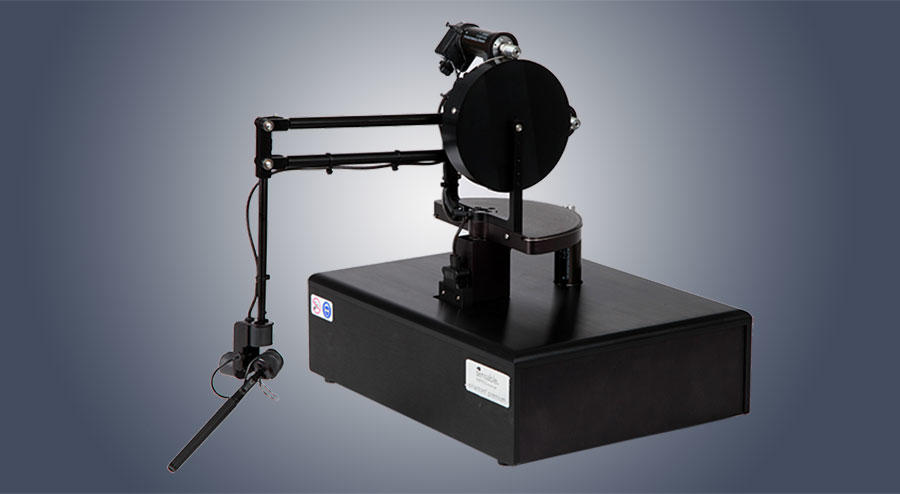
\includegraphics[width=0.6\linewidth]{phantom}
		\caption{The Phantom Premium Haptic Device https://www.3dsystems.com/haptics-devices/3d-systems-phantom-premium}
		\label{fig:phantom}
	\end{figure*}		
	
	%with the user controlling the device, which reports the state to a virtual environment
	
	 %physics engine in order to determine the interaction force to be rendered back to the user. Haptic algorithms must balance stability, transparency, and the renderable impedance range. 
		
	The haptic controller needs to consider the accuracy of the rendering of the interaction forces, the stability of the system, and safety of the user. The modelling and the physics of the virtual environment must also be considered. 		
		
		Early haptic algorithms used penetration depth between the device and virtual object to determine the interaction forces. However, this leads to ambiguities regarding what surface of the object the user is interacting with (in other words, what face the interaction force should be normal to). In \cite{Zilles}, the God-Object method is introduced to resolve this issue. The device is given a virtual position, that which it would take if the haptics could be infinitely stiff (\textit{i.e.} it always remains at the surface of the object) -- in this way the direction of the interaction force is always known. 
		
	A third option is given in \cite{Adams1999}, known as the haptic coupling. This coupling is a virtual system placed in between the physical device and the virtual environment. The purpose is twofold: to decouple the design of the virtual environment and the controller, and to allow for different control and environment causality combination (\textit{e.g.} an admittance based robot could have an impedance based virtual environment). It in effect places limits on the range of impedances that can be rendered (how close to a rigid wall or free space the device can simulate), because rendering an impedance out of the renderable range of the device can lead to instability. 
	
	%Fig. \ref{fig:haptic_adm} shows a simple system containing the operator, the robot or haptic interface, and the virtual environment. Without the haptic coupling, the virtual environment must have the same causality as the controller in this case an admittance causality. Therefore the physics of the environment must calculate the virtual position based on a 
	
	%For example, an admittance controlled haptic device is shown in Fig. \ref{fig:haptic_adm}. In this example, the virtual environment is the control algorithm, it is restricted ... More information on the haptic coupling is given in Sec. \ref{sec:haptic}.
	
	\begin{figure*}[t] 
		\centering
		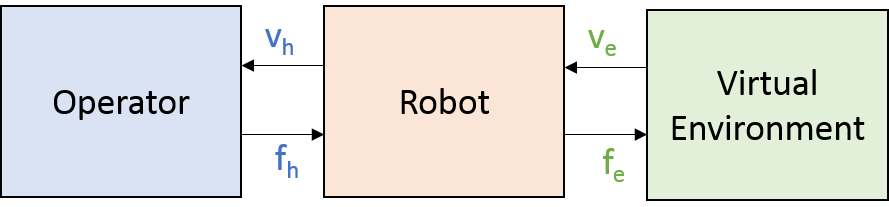
\includegraphics[width=0.75\linewidth]{haptics_admittance}
		\caption{Block diagram of an admittance haptic device}
		\label{fig:haptic_adm}
	\end{figure*}	
	
	\begin{figure*}[t] 
		\centering
		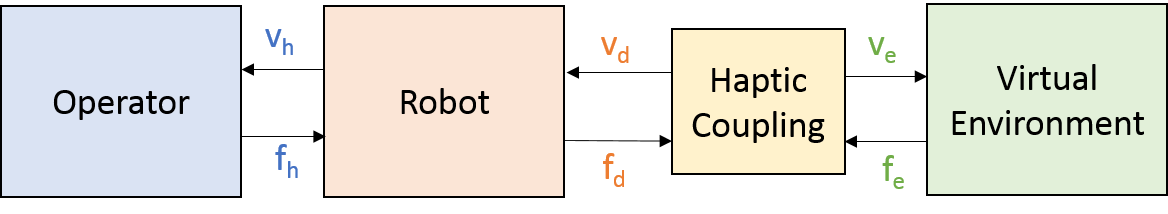
\includegraphics[width=0.75\linewidth]{haptic_admittance_coupling}
		\caption{Block diagram of an admittance haptic device}
		\label{fig:haptic_adm_coup}
	\end{figure*}	
	
	
\section{Interviews and Shadowing}

%------------------------------------------------------------------------
%-shadowing notes
%
%-------------------------------------------------------------------------
	
	The rise of the human-centred design paradigm underscores the importance of involving end users in the design process, especially when the designers lack expertise in the field of interest. After the literature review, the next step of the design process was to consult the end user and collect qualitative data and advice. In the case of rehabilitation robots, there are two types of end-users: the stroke patient using the device, and the therapists who decide when and how to incorporate the device into their rehabilitation regimen. The therapist, however, has greater expertise with stroke rehabilitation in general, and will ultimately be the one who decides the device's fate on the stroke ward. Therefore, it was decided to interview and shadow several PT's and OT's concerning the direction of the project. Patient's were not consulted, due to their lack of expertise in stroke rehabilitation, although their input will be vital in future evaluation experiments. 
	
	Fieldwork was conducted at the Civic campus of the Ottawa Hospital (TOH), in cooperation with Dr. Dariush Dowlatshahi, and with ethics approval from the Ottawa Health Science Network Research Ethics Board (OHSN-REB). Three PT's and two OT's were recruited for two days of interviews and shadowing. Inclusion criteria included experience working on the stroke ward delivering rehabilitation to stroke patients. Not enough data was collected to perform any meaningful statistic -- instead, key insights guided the fundamental concept of the device, and information was gathered not otherwise available through a literature review. Some topics of interest included:
	
	\begin{itemize}
		\item Typical acute, bed-bound rehabilitation 
		\item Patient Engagement -- how the therapists keep patients motivated and actively participating 
		\item The hospital environment
		\item The therapists' views on rehabilitation robotics 
	\end{itemize}

	
	\subsection{Typical Rehabilitation}
	
	Bed-bound lower-limb rehabilitation is one of the first therapeutic activities administered at the stroke ward, and it continues to be used even after patients are mobile. Bed-bound exercises tend to be simple movements, including knee flexion/extension, leg lifts, hip adduction/abduction, and ankle rolls. All exercises involve the therapist manually manipulating the patient's leg, providing assistance to whatever extent the therapist deems necessary. If the patients are advanced, the therapist may choose to resist motion instead of assisting. 
	
	Parameters from typical rehabilitation will help determine the requirements of the new robotic system. Therapists estimated that they exert a maximum of 10 - 15 lbs of force to the leg. The range of motion of patients varied, but many could go through the full range of the leg. The exercises were done slowly at a consistent speed. The role of the therapist can be summarized as providing support to leg and providing assistance through the motion. 
	
	Some patient's are capable of performing bed-bound exercises independent of the therapist. Performing independent practice can increase total rehabilitation dosage and is recommended by stroke guidelines \cite{Hebert2016}. However, some patients who are either at an earlier stage of recovery or have suffered more severe strokes are incapable of performing bed-bound exercises without assistance, and so their total dosage is limited to time spent with the therapist. 
	
	\subsection{Patient Engagement} 
	 It is important for the patient to be actively engaged in the exercise. Therapists will try to only provide assistance as needed, by waiting for the patient to initiate the movement. Many of the patients required verbal or physical engagement throughout the process. This is in part due to a phenomenon known as neglect, wherein the stroke victim has trouble focusing on the effected side of the body. Therapists will verbally motivate patient's in a manner similar to a personal trainer; otherwise they may engage the patient in conversation. Physical or tactile cues can be used to guide the patient, for example by tapping the leg if it needs adjusting. Sometimes, pictures and posters (\textit{e.g.} of cats and dogs) were posted in front of the exercise machines in the therapy room. Another common practice is to switch to a new exercise if the patient is showing signs of losing focus. 
	 
	 \subsection{Hospital Environment}
	Space in the hospital is limited. Many rooms house four patients, and are often crowded by hospital staff, family, and equipment. The beds themselves vary in model and size, but all have some common characteristics: movable guards on the side, removable baseboard, and a tiltable frame controlled from a panel. There appear to only be outlets behind the beds near the floor, but this will again vary from room to room. 
	There is also a therapy room where more advanced patients go to practice sit-to-stand, walking, stair-climbing, etc. This room is more spacious and also includes beds (albeit simpler beds that cannot be tilted and that do no have guards). 
	
	\subsection{Therapy Schedule}
	
	Therapists generally have a high workload and so must carefully schedule time with patients. At this particular hospital, patients received on average 30 minutes every other day with a physiotherapist for lower-limb rehabilitation. Most patients were fatigued by the end of the session, and so increasing the duration beyond 30 minutes is not feasible. However, the therapists recognized that the patients could benefit from more sessions throughout the week. Some activities that are physically burdensome need two therapist, or more often a therapist and an assistance. These activities are even more difficult to schedule.
	
	\subsection{Other Comments and Concerns}
	
	Most therapists had concerns over safety. They recognized that the robot could potential apply forces which could harm the patient. One point of concern was rotation of the leg out of position such that the force was applied incorrectly. For example, during the knee flexion/extension exercise, if the leg were to rotate out of the sagittal plane, the robot could apply a torque about the hip which would bend the leg further and potentially injure the patient. Therapists suggested having multiple support points along the leg to keep the leg in position. 
	
	Other comments included the need for comfort, particularly using comfortable material where the robot and human interact. They also mentioned the use of tactile methods of engaging the patient (\textit{e.g.} tapping or vibrations applied to the leg). Some indicated that combining upper and lower-limb activities could be beneficial (\textit{e.g.} by using a joystick with the robot). 
	
	
\section{Device Concept} 

With ViGRR, our goal was to design a lower-limb rehabilitation robot targeting acute patients by creating a device compatible with a patient who is lying or reclined in a hospital bed. ViGRR accomplishes this, and has been validated on healthy subjects. However, some aspects of ViGRR prevent it from being used easily in the hospital, including its high weight, high power, and size. The next stage in the project is to repackage ViGRR into a more accessible and light-weight design. 

This new prototype should align with ViGRR's fundamental concept: a lower-limb robot capable of assisting bed-bound acute stroke patients with rehabilitation. The device should be a viable tool for therapists within the hospital to use to increase functional outcomes for their patients. It should replicate the role of the therapist when providing assistance for bed bound exercises. There are three primary roles:

\begin{enumerate}
	\item Support the leg 
	\item Provide assistance through the motion
	\item Engage the patient
\end{enumerate}

Supporting the leg will be accomplished through the physical structure of the device. Assistance will be provided using force feedback and interaction controllers which can ensure that the patient is contributing to some extent. The patient will be engaged using virtual environments and haptic feedback. 

%Bed-bound exercises include a variety of simple movements, such as leg lifts, knee extensions, and hip abductions. Since this device is a proof-of-concept, it was decided that we would initially target a single exercise, evaluate its performance in the hospital, and then extend to target other exercises by adding degrees-of-freedom. We chose the knee flexion/extension exercise for the following reasons:

%\begin{itemize}
%	\item It is a commonly used bed-bound exercise
%	\item It is important due to its relation to the sit-to-stand activity, which is the first stage of getting the patient mobile
%\end{itemize}
 
%The knee flexion/extension exercise requires just a single horizontal degree-of-freedom. The therapist uses one hand to support the leg under the knee, and the other hand to support the foot and apply force through the heel. They slowly move the leg back and forth, encouraging the patient to push. They are careful to keep the leg aligned in the sagittal plane. 

There are several use cases for the device. The therapist could use it during therapy instead of manually moving the legs. This would relieve them of the physical burden, the virtual environments may encourage the patient to participate more, and the data collected could be used to track progress. The therapist could use multiple devices simultaneously to provide care to multiple patients. This would allow them to see more patients and thus increase therapy dosage. Finally, since the device replicates the role of the therapist, the device could be used separately from the therapist, under the supervision of other hospital staff. This would encourage patient's to practice independently, thereby increasing therapy dosage. 

In addition to these requirements, the device should be usable within a hospital environment. The device should be safe such that the patient is not harmed, and should also be perceived as safe so that the therapists and patients are willing to use it. The device should fit on a hospital bed, and should be lightweight and small enough to be manageable within a hospital room. The set-up of the device should be quick and easy.



%---
%We set out to design a simple lower-limb rehabilitation for acute, bed-bound stroke patients. We chose to design for the knee flexion-extension exercise because it is most related to sit-to-stand, which is the most important activity for bed-bound patients to recover as it allows the patient to get up and begin gait rehabilitation. The robotic configuration best suited to this exercise is a one degree of freedom linear actuator. 


%Stroke rehabilitation best practices were outlined in the previous section. A few key recommendations highlight the potential benefits of introducing a simple-to-use robotic device into the rehabilitation arsenal. The robotic device would primarily be used to offer additional rehabilitation time to patients under the supervision of a nurse or other responsible person. The gaming aspect of the system would ensure the patient is engaged in the exercise, and also offer feedback so that the patients movements can be regulated even in the absence of a therapist. The games and visualizations could also be tailored to simulate ADL's. Therefore, a robotic device could theoretically boost outcomes by covering the following recommendations:



\section{Contributions and Outline}

A one DOF robot was designed and created according to the requirements determined from the literature review, shadowing, and previous work on ViGRR. The device consists of a DC motor, force sensor, belt drive, footplate, frame, and a number of smaller components. A printed circuit board (PCB) was created to route signals, do preprocessing, and distribute power. System software was implemented on a real-time linux system. A controller was created in C, which can operate the device using admittance control, haptic feedback, a basic physics engine, communication with a UI server, and data logging. Real time functionality is ensured using POSIX standards for memory locking, multi-threading, etc. The UI is implemented as website using the React framework, and some simple games are created using the THREE.js 3D web graphics library. The controller was designed as a modular system that can be easily re-factored to accommodate design changes in future iterations. The device was evaluated through a number of tests and experiments, including functional tests, safety tests, and an pilot study with healthy subjects. The results show that the device functions as planned, but that several things must be changed/added before it is ready for patient testing in the hospital.

	\begin{figure*}[h] 
		\centering
		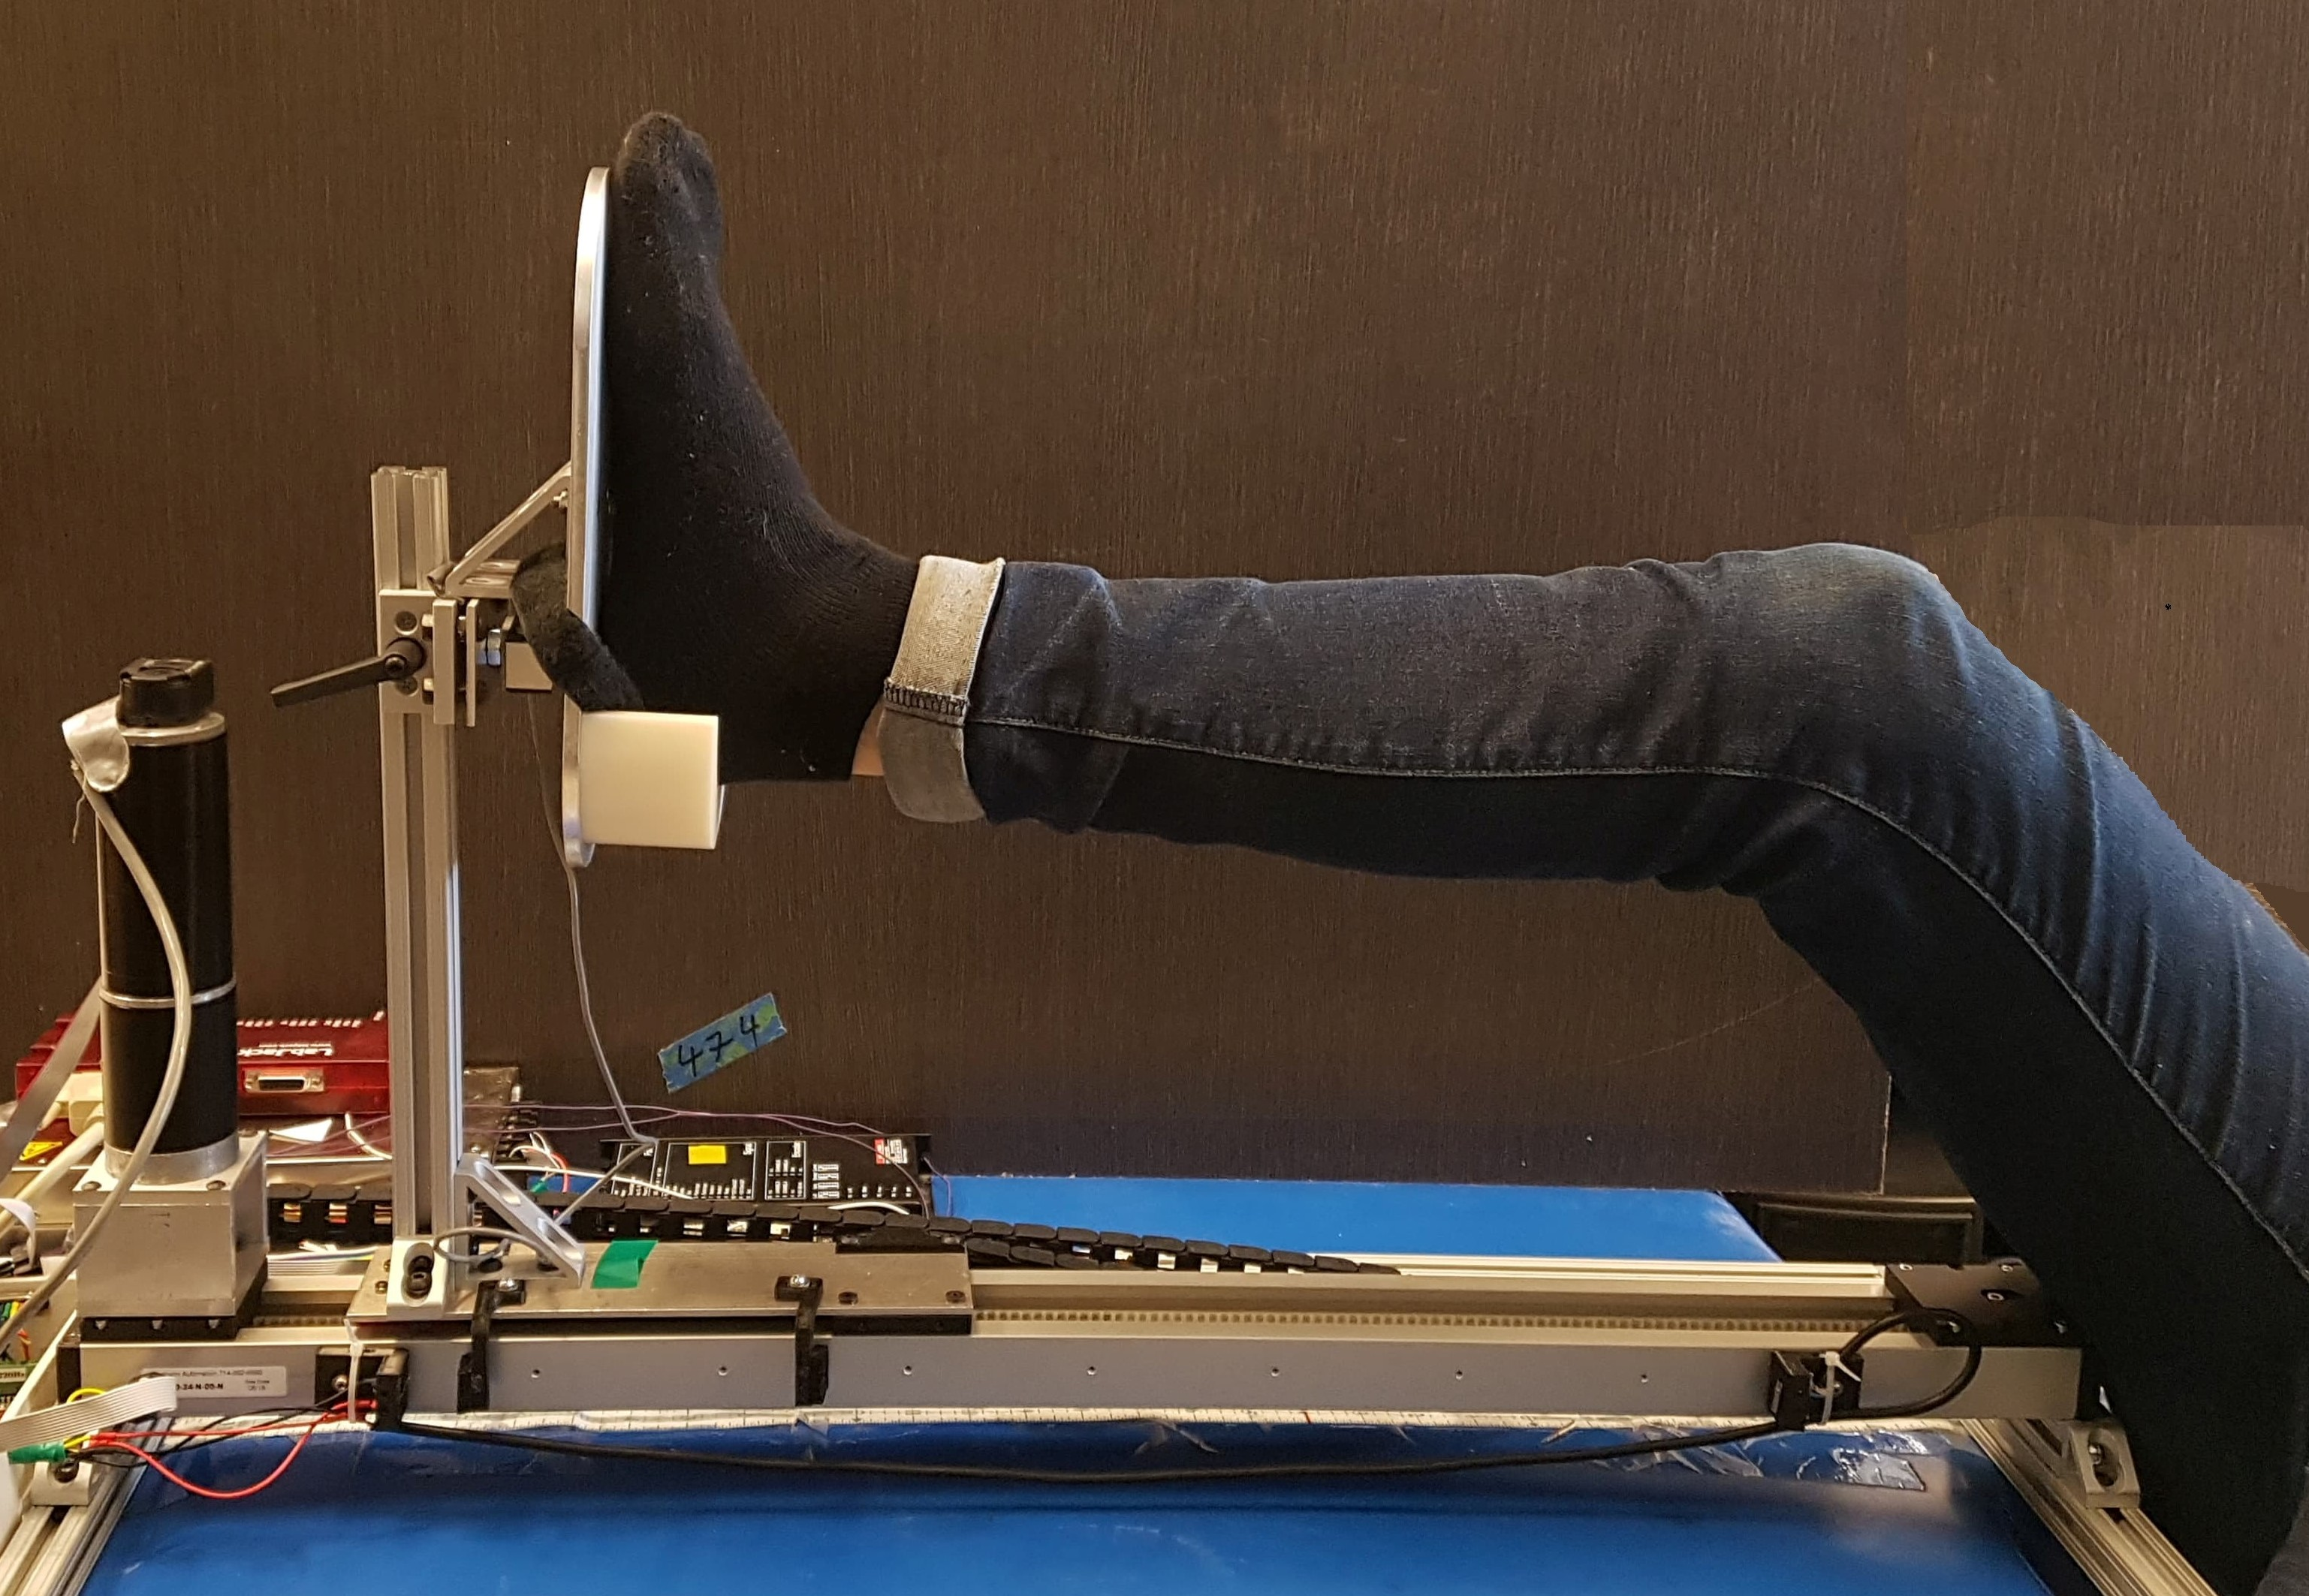
\includegraphics[width=0.75\linewidth]{robot_leg}
		\caption{The Rehabilitation Robot with User's Leg}
		\label{fig:robot_leg}
	\end{figure*}
	
	\begin{figure*}[h] 
		\centering
		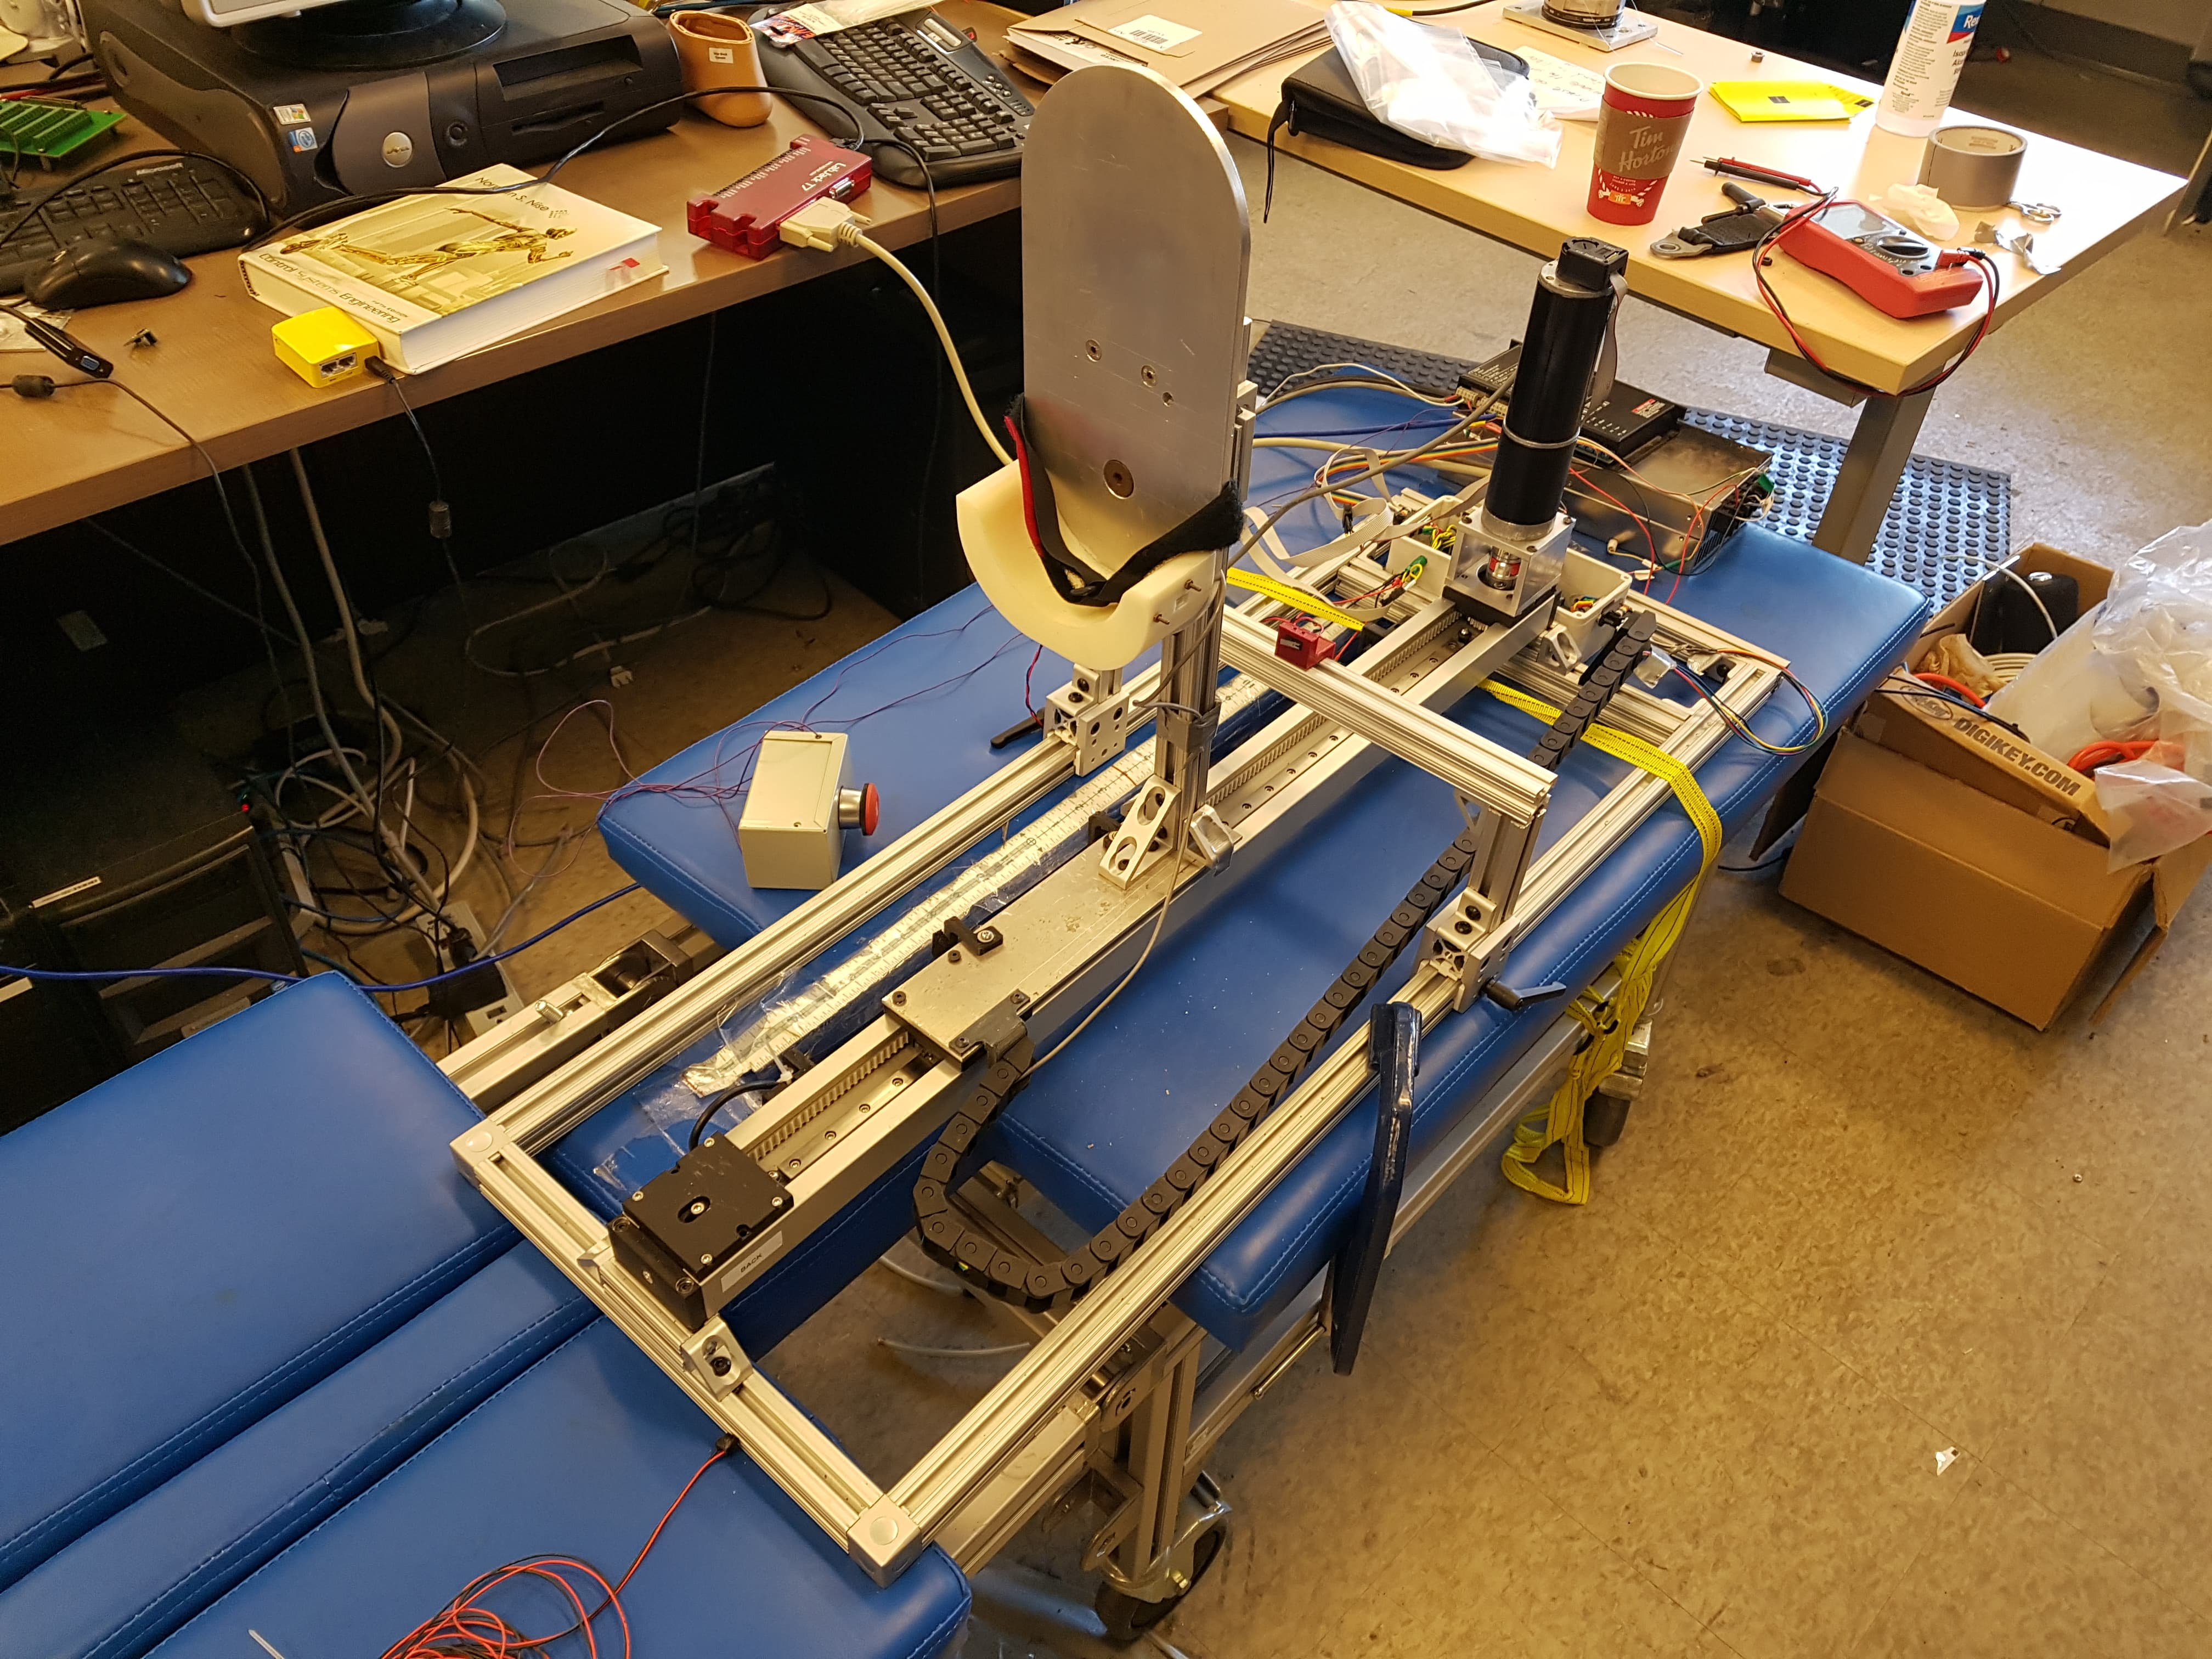
\includegraphics[width=0.75\linewidth]{device_on_bed}
		\caption{The Rehabilitation Robot on the test bed}
		\label{fig:robot_on_bed}
	\end{figure*}



\begin{itemize}

\item Chapter 2 covers the design of the device. This includes preliminary design choices, the design of the physical structure, the actuation and sensors, the design of the electronics (power distribution, signal routing and preprocessing), and the chosen computer hardware. 

\item Chapter 3 covers the controller and its implementation in the software, including the basic admittance control, and the haptic feedback with physics engine. The design of the user interface (UI) and some basic games/visualisations are also discussed. The communication and the overall software design within real-time Linux is explained, including the how the modular design will allow it to be easily adapted to future design iterations. 

\item Chapter 4 covers testing and experiments, including functional testing of the software, controller, and UI. The methods and results from a small study on healthy subjects are presented, with questionnaire answers regarding the subjective experience of participants, along with quantitative performance metrics. 

\item Chapter 5 concludes with a summary of contributions and recommendations for future work. This includes features that were required which have not yet been implemented due to time constraints, and ideas for future direction of the project. 


\end{itemize}


\chapter{Device Design and Implementation} \label{ch2}

	\section{Design Iterations}
	
	This rehabilitation robot was designed from scratch, from the initial concept to the final realization. This sections lists the early design decisions and iterations, along with the justification. There were four significant design decisions to be made:
	
	\begin{enumerate}
		\item The number of degrees of freedom (DOF) in the robot. The final decision was to use one linear DOF.
		\item The type of linear actuator to use. Options included pneumatics, ball screws, and belt drives; the final design uses a belt drive.
		\item The robots placement within the room (on the bed v.s. beside the bed). The final design sits on the bed.
		%\item The conceptual design of a secondary leg support which would prevent the leg from rotating out of position. This was never realised, however the design is presented here for future work. It consists of a 3 DOF passive linkage which can follow the leg through the motion and provide lateral support. 
		\item The controller can be run from either a microcontroller or a full computer. Due to the plans to increase complexity in the future, as well as the need for a user interface, a computer was chosen. 
	\end{enumerate}
	
	
		\subsection{Degrees of Freedom}
		
		This project is a continuation of ViGRR, a 4 DOF planar robot. The goal is to repackage ViGRR in a smaller form more compatible with the hospital. However, we also wanted feedback from both patients and therapists at the hospital throughout the design. It was decided to build a smaller, simpler robot, which could be taken to the hospital and tested promptly. Feedback could then be used to extend the simpler robot with additional DOF's in order to achieve more complex movements.
		
		There were three options for a simpler robot configuration: 1 linear DOF, 1 rotary DOF, or 2-DOF. The primary motions we need to target include circular, horizontal linear (knee extensions), vertical linear (leg lifts), and more complex movements like gait trajectories. These also need to be adjustable to accommodate a variety of body sizes. A linear DOF could target knee extension or leg lifts, whereas a rotary DOF would only be able to target a weak approximation of a gait trajectory (\textit{i.e.} a circular motion more similar to pedalling a bike). A 2 DOF system could accomplish more types of motions, for example doing both leg lifts and knee extensions, or more closely approximating a gait trajectory.
		
		Ultimately the single rotary DOF was excluded because its movement was not relate to any of the bed-bound exercises. The 2-DOF was excluded because \textit{(a)} it was determined to be too complex for the scope of this thesis, and \textit{(b)} it was decided the final configuration of a multi-DOF device would be left to future iterations after receiving feedback from the hospital. Therefore, the final design is a single horizontal linear DOF. 

					
		\subsection{Linear Actuator Type}

	There are several ways of actuating a linear motion. This includes hydraulics \& pneumatics, ballscrews, and belt drives.
	
	\textbf{Hydraulics \& Pneumatics}: Hydraulics and pneumatics use pressurized liquid or air to achieve linear actuation. They require more consideration than other off-the-shelf solutions, such as ...


	\textbf{Ballscrew}: Ball screws offer high precision and very low backlash. However, the rehabilitation needs to move quickly, and so the ballscrew would require a very large pitch, or the motor would need to powerful enough to supply high torque at high speed. Cost restraints therefore make using a ballscrew impractical. 
	
	\textbf{Belt Drive}: Belt drives are in general less expensive and can achieve high speeds. However, the belt introduces flexibility into the actuator which may affect the precision of the controller. However, precision in this application is not imperative since small errors will not be perceived by the patient. Furthermore, flexibility and belt slip at high torques could actually act as worst-case safety measures. Ultimately an off-the-shelf belt drive was used in the design (Fig...).


	
	\begin{table}[]
	\centering
	\caption{Benefits of Actuator Types (x = benefit)}	
	\begin{tabular}{|l|c|c|c|c|}
		\hline
		\textbf{Type} & \textbf{Cost} & \textbf{Ease of Setup} & 		\textbf{Backdrivable} & \textbf{Precision} \\ \hline
		Ballscrew &  &  & x & x \\ \hline
		Belt Drive & x & x & x & \\ \hline
		Pneumatic/Hydraulic & x &  & x & \\ \hline
		\end{tabular}
	\label{tab:actuator}
	\end{table}
				
		
		\subsection{Placement Relative to Bed}
		
		%%include sketch 
			
	\begin{figure*}[t] 
		\centering
		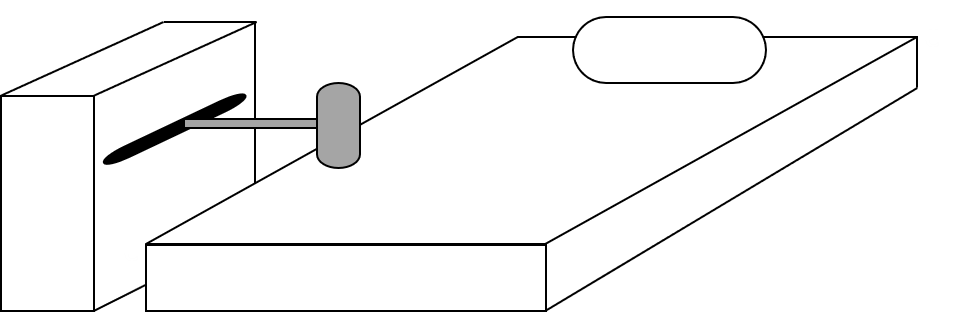
\includegraphics[width=0.75\linewidth]{off-bed}
		\caption{Off-bed Design}
		\label{fig:off-bed}
	\end{figure*}	
	
	
		
	\begin{figure*}[t] 
		\centering
		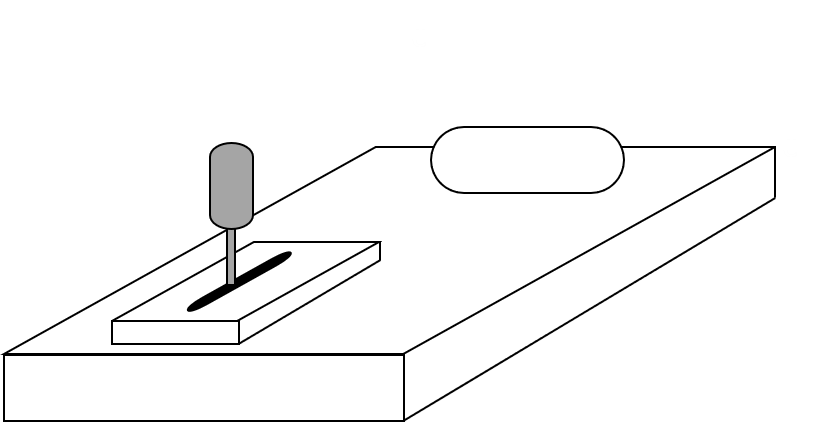
\includegraphics[width=0.75\linewidth]{on-bed}
		\caption{On-bed Design}
		\label{fig:on-bed}
	\end{figure*}	
	
		
		The device needs to support the patient's leg and provide horizontal assistive forces through the leg flexion/extension exercise. Several possible structural configurations were identified. The device could sit beside the bed, with the foot plate extending horizontally to support the patient's foot (see Fig \ref{fig:off-bed}). The device could sit on the bed, under the patient's leg (see Fig \ref{fig:on-bed}), similar to a passive range of motion machine. Each configurations has pros and cons, as listed in Table. \ref{tab:config}.

		
	\begin{table}[] \label{tab:config}
	\centering
	\caption{Structural Configuration }	
	\begin{tabular}{l|l|l}
		\hline
		& \textbf{On-Bed} & \textbf{Beside-Bed}  \\ \hline
		\textbf{Pros} & Takes less space in room  & Easy to set up  \\ 
		 & Better support of patient's leg  & Easier to extend DOF's \\ \hline
		 \textbf{Cons} & Harder to set up  & Requires room beside bed \\ 
		 & May obstruct patient  & Large moment on footplate \\ 
		 & & Must move patient to edge of bed \\ \hline

		\end{tabular}
	\label{tab:structure}
	\end{table}
		


	The deciding factors were the moment applied by the leg on the footplate, and the space in the room. Two forces are created by the user: the applied force pushing or pulling the footplate ($F_a$), and the weight of the leg on the heel support ($F_w$). The on-bed design sits under the leg, so the moment created by the weight of the leg and its moment arm ($R_x$) can be minimized by minimizing the $R_x$ (Fig. \ref{fig:on-bed_moment}). If the device sits beside the bed, the footplate must extend horizontally outwards, resulting in the weight of the leg creating a moment on the actuator throught that distance ($R$), which is harder to minimize (Fig. \ref{fig:off-bed_moment}). The length of the footplate extension can be shortened to reduce the moment, however this would require that the patient is transferred closer to the edge of the bed, which is both time consuming and possibly hazardous. Additionally, the device would require room beside the bed. After observing several hospital rooms in the stroke ward, it was clear that this space is not always available, due to equipment, furniture, and crowded rooms which can contain up to four beds. The on-bed design sits completely on the bed and so should be compatible with any room. The moment applied to the footplate due to the weight of the leg is smaller as it supports the leg from below. Finally, it can be positioned on the bed in a way that suits the patient, instead of having to move the patient to the edge. 
	
	\begin{figure*}[h] 
		\centering
		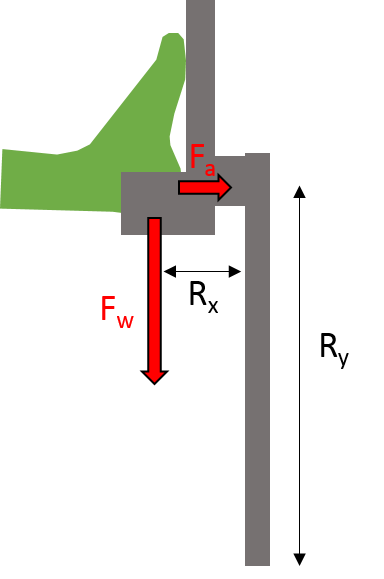
\includegraphics[width=0.3\linewidth]{on-bed_moment}
		\caption{Forces and moment arms for on-bed design}
		\label{fig:on-bed_moment}
	\end{figure*}
	
	
	\begin{figure*}[h] 
		\centering
		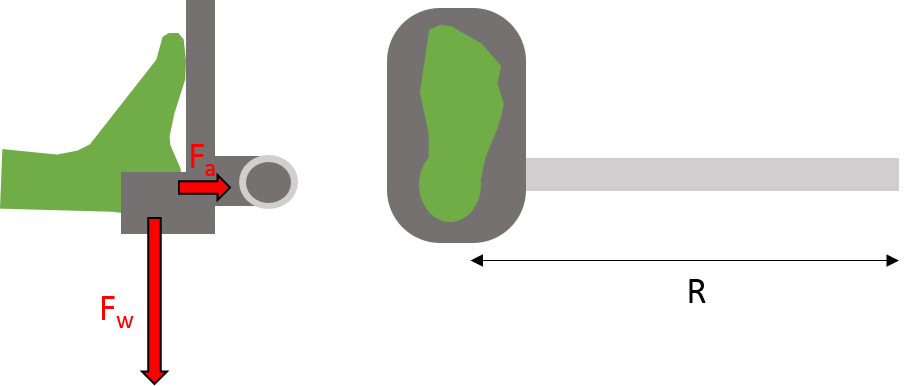
\includegraphics[width=0.6\linewidth]{off-bed_moment}
		\caption{Forces and moment arm for off-bed design}
		\label{fig:off-bed_moment}
	\end{figure*}
	
	
	\subsection{Computer v.s. Microcontroller}
	
	The controller can be executed either from a microcontroller or from a full computer. The microcoontroller is cheaper, easier to set up for real time code execution, and has built in I/O's. Computers have more processing power, memory, can easily be networked or connected wirelessly, but require external data acquisition. Special care must be used to set up a real time system which can execute control loops with minimized latencies. 
	
	For a 1-DOF device, a microcontroller is the typical choice given that the control is simple and does not require much processing power or memory. However, eventually extra DOF's may be added to our system to the point where a microcontroller is not suitable. The computer could also be used to run the user interface (UI). Therefore we chose to use a computer to run the control software. 


		
	%\subsection{Secondary Leg Support}
		
	%When therapists assist patients with the knee extension exercise they support the patients leg at two points: at the heel and under the knee. From the heel they hold the leg and apply force to assist or resist the motion. The hand under the knee also supports the leg, and keeps the leg from rotating out of plane. 
	
	

	\section{Device Overview}
	
	The final design consists of one linear degree of freedom, actuated by a belt drive, which sits on the bed under the patient's leg. The footplate has heel support and a Velcro strap to keep the foot in place, and is height adjustable to accommodate a variety of leg sizes. There is also an adjustable end stop to limit the length of the stroke, which can be customized to each individual in order to prevent leg over-extension. Figure \ref{fig:cad} shows a CAD rendering of the design with the frame, footplate, and actuator. Figure ... shows the device as of July 2019.

	\begin{figure*}[h] 
		\centering
		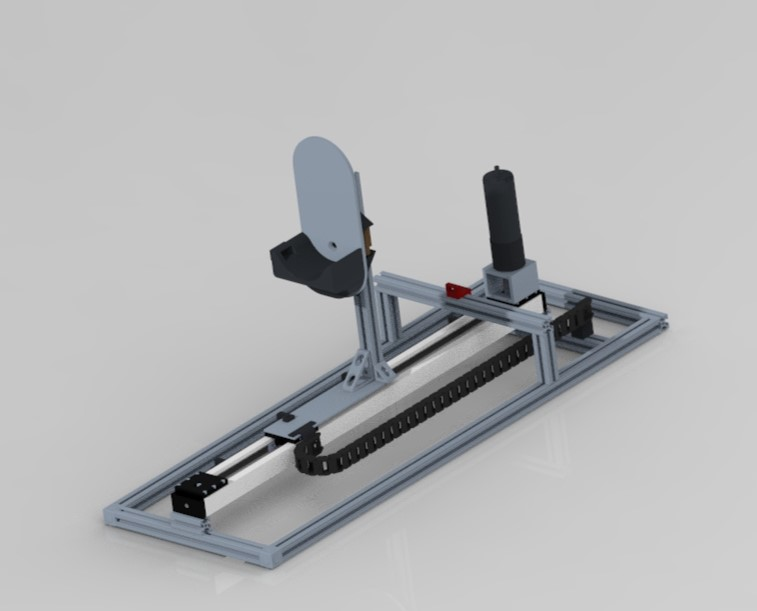
\includegraphics[width=0.75\linewidth]{overall_device}
		\caption{The rehabilitation device}
		\label{fig:cad}
	\end{figure*}
	
	
	\section{Structural Design}
	
	\subsection{Frame}

	The frame holds the actuator, footplate, and electronics (Fig. \ref{fig:frame}). It should fit on a bed, under one of the patient's leg, without obstructing the other leg or the patient's body. The frame is constructed out of 1x1' aluminium profile. The frame can be clamped or strapped to the bed to secure it in place. Future designs could include custom mounts to specific beds by attaching to the footboard or sides. The frame also contains an adjustable physical end stop which is used to control the maximum stroke length of the actuator. This can be adjusted to prevent over-extension of the leg.
	

	\begin{figure*}[h] 
		\centering
		\includegraphics[width=0.75\linewidth]{frame}
		\caption{The structure of the frame}
		\label{fig:frame}
	\end{figure*}
	
	
	
	\subsection{Footplate}
	
	The footplate attaches to the belt drive and is height adjustable. The footplate both supports the leg and is a the interface through which the robot and user interact. It is shown in Fig \ref{fig:footplate_label}. An aluminium profile extends from the base on the belt drive. An off-the-shelf carriage with a handle lock is used to adjust the height. Mounting plates are used to attach a load cell to the carriage, which is placed near the bottom of the footplate. The footplate is cut from aluminium 1/8'' plate. 
	

	
	\begin{figure*}[h] 
		\centering
		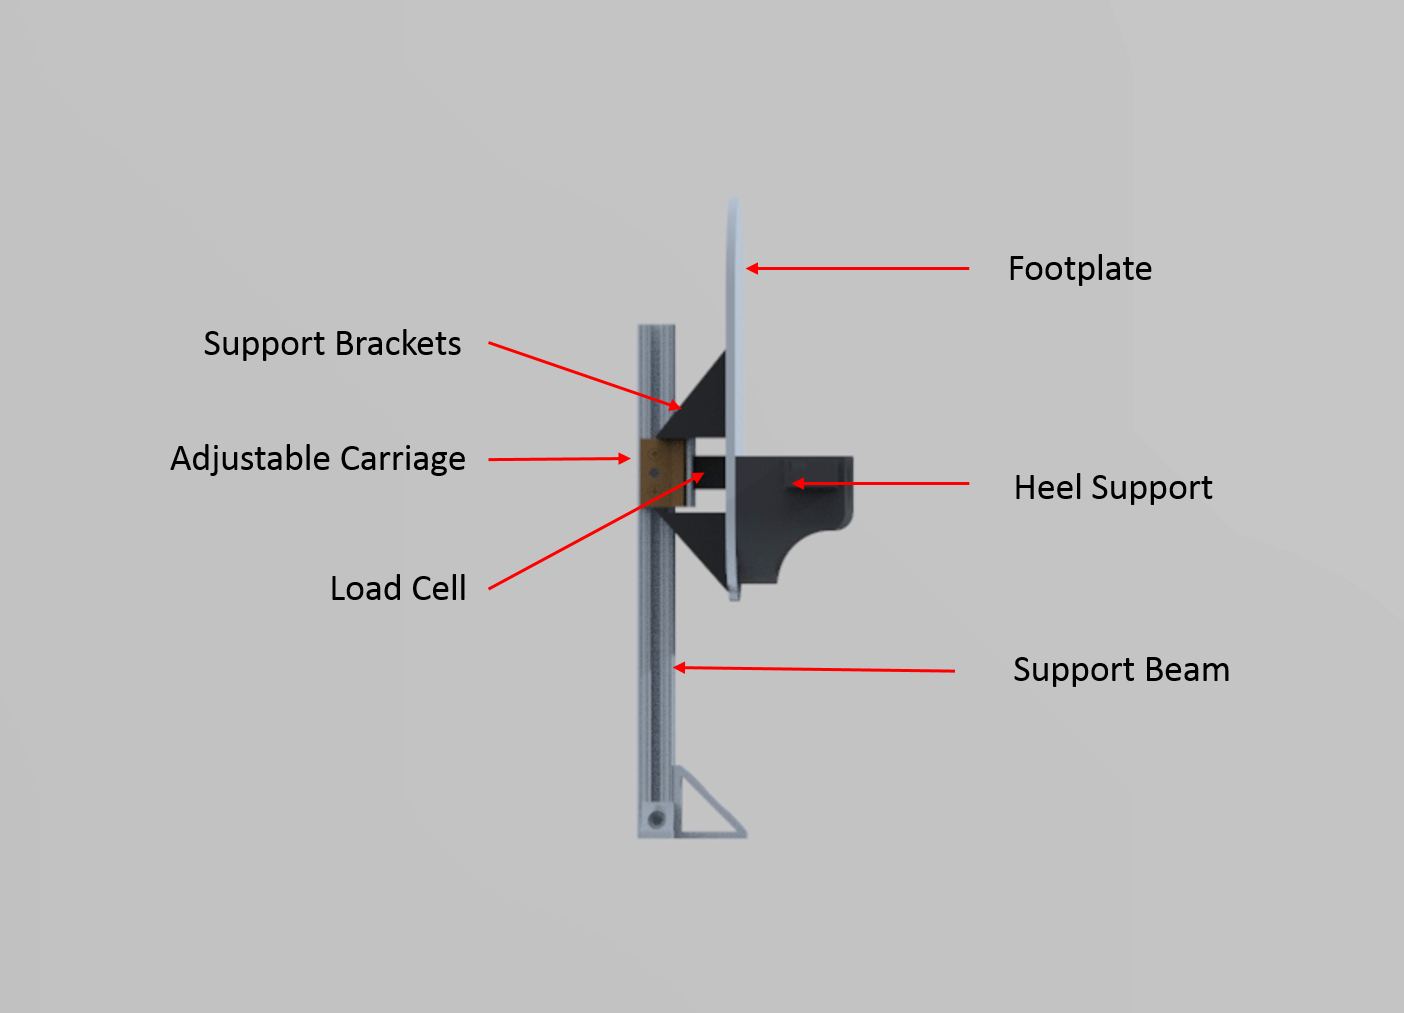
\includegraphics[width=0.5\linewidth]{footplate_label}
		\caption{The structure of the footplate}
		\label{fig:footplate_label}
	\end{figure*}
	

	The load cell measures force applied horizontally; however it may also register force due to moments placed on the footplate either from the weight of the leg or from applying forces near the top of the footplate. To minimize these erroneous measures, support brackets were created to transfer vertical forces from the footplate directly to the adjustable base, thereby reducing the effect of the moment. These brackets are shown in fig REF, and were 3D printed with PLA. To hold the foot in place, a custom heel support was created (Fig REF). It contains housing for an infra-red sensor which can detect whether the foot is in place for safety. The heel support was also 3D printed, using ABS for additional strength. 
	
	\section{Hardware}
		\subsection{Actuator}	
		
	\begin{figure*}[h] 
		\centering
		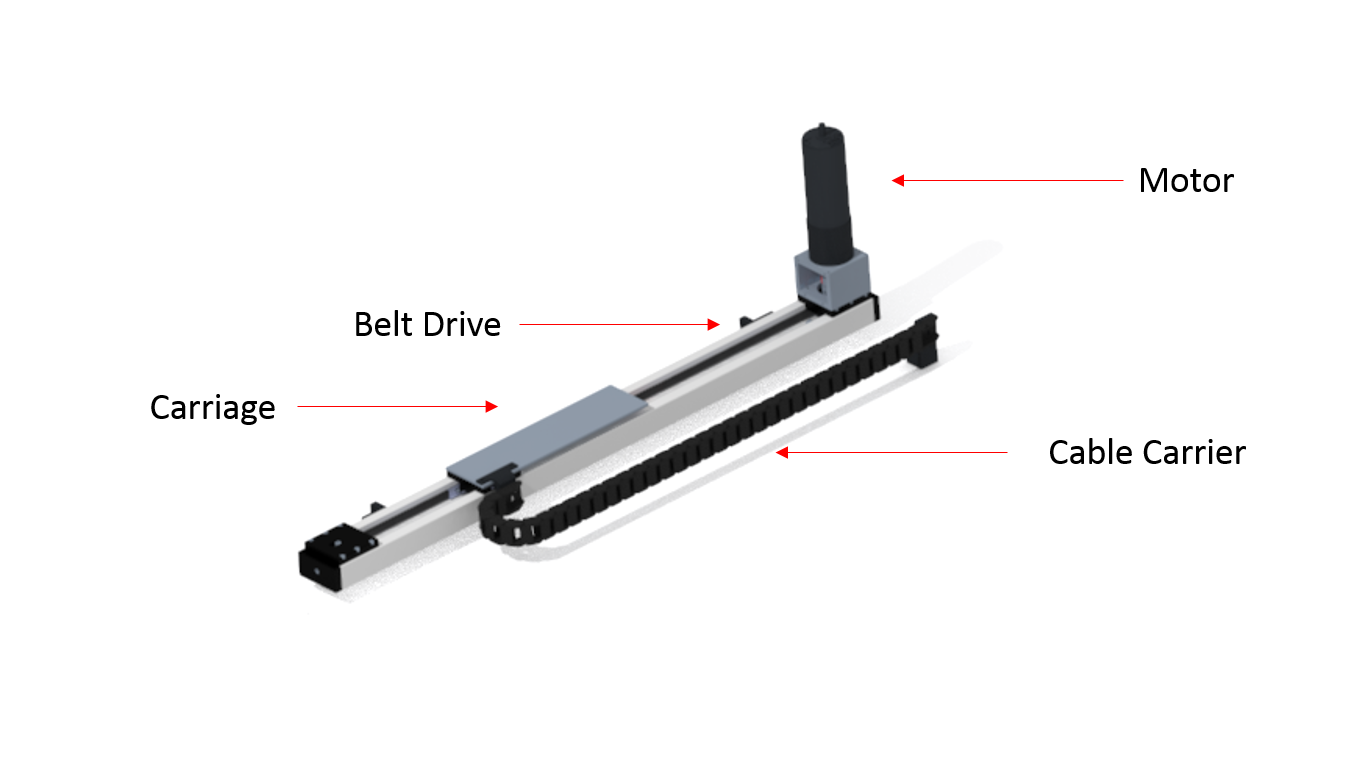
\includegraphics[width=0.75\linewidth]{actuator}
		\caption{The belt drive and motor}
		\label{fig:actuator}
	\end{figure*}
		
		
	The system is actuated using a Brushed DC Motor, gear reduction, coupling, and an off-the-shelf linear belt drive (Fig. \ref{fig:actuator}). The Brushed DC Motor is a Maxon RE 50 200W Graphite Brush model (part number 370354). The gear reduction is the Maxon GP 52C Planetary Gearhead (part number 223090). The coupling is an Aluminium Flexible Shaft Coupling with a polyurethance spider from McMaster-Carr. The linear belt drive is a LB250-24 Belt Drive from Anaheim Automation. The motor is mounted to the belt drive using custom machined aluminium mounts. Finally, a cable chain is used to secure wires running from sensors on the footplate to the electronics box mounted at the base of the device. 
	
	

	\subsubsection{Motor Specification}
	
	\begin{table}[h]
	\centering
	\caption{DC Motor Properties}	
	\begin{tabular}{|l|l|}
		\hline
		\textbf{Property} & \textbf{Value}  \\ \hline
 		Nominal Voltage & 24V  \\ \hline
 		Torque Constant & 38.5 mNm/A \\ \hline
 		Speed Constant & 248 rpm/V  \\ \hline
 		Stall Torque & 8.92 Nm \\ \hline
 		Nominal Speed & 5680 rpm \\ \hline
 		Nominal Torque & 405 mNm \\ \hline
 		Reduction & 53:1  \\ \hline
 		Max Speed Input & 6000 rpm  \\ \hline
 		Max Torque Input & 45 Nm  \\ \hline
		\end{tabular}
	\label{tab:motor}
	\end{table}
	
	
	\begin{table}[h]
	\centering
	\caption{Belt Drive Properties}	
	\begin{tabular}{|l|l|}
		\hline
		\textbf{Property} & \textbf{Value}  \\ \hline
		Stroke Length & 24 in  \\ \hline
 		Travel per Revolutions & 4.8 in/rev  \\ \hline
 		Maximum Travel Speed & 100 in/s  \\ \hline
 		Static Load capacity & 1000 lb  \\ \hline
 		Dynamic Load Capacity & 200 lb  \\ \hline
 		Pulley Radius & 35 mm  \\ \hline
		\end{tabular}
	\label{tab:belt}
	\end{table}
	

	
	The motor is required to move the actuator fast enough while also be able to apply adequate levels of force fro assistance or resistance. This motor and gear assembly was used from a previous project, and was found capable of fast of linear motion and applied force. The maximum linear speed is in this case limited by the maximum input RPM to the gearhead, 6000RPM: 
	
	\begin{align*}
		V_{max} &= \frac{p\omega _{max}}{GR} \frac{1min}{60s} \\
		&= \frac{(0.122m)(6000 RPM)}{(53)} \frac{1min}{60s} \\
		&= 0.230 m/s
	\end{align*}
	
	The nominal torque and speed are used to estimate the nominal linear speed and its associated nominal applied force:
	
	\begin{align*}
		V_{nom} &= \frac{p\omega _{nom}}{GR} \frac{1min}{60s} \\
		&= 0.217 m/s
	\end{align*}
	\begin{align*}
		F_{nom} &= \frac{\tau _{nom}GR}{R_{pulley}} \\
		&= \frac{(0.405Nm)(53)}{0.0175} \\
		&= 1227N = 275 lbs
	\end{align*}

The maximum speed of 230 mm/s is adequate for our purposes, as the system is designed for stroke rehabilitation which is a slow moving process. The nominal force of 275lbs is much higher than the assistive forces seen during traditional therapy (which therapists estimate to be up to 20 lbs). In the future, a lower gear reduction could be used to increase the maximum speed to accommodate more advanced patients.

	\begin{table}[h]
	\centering
	\caption{System Maximums}	
	\begin{tabular}{|l|l|}
		\hline
		\textbf{Property} & \textbf{Value}  \\ \hline
 		Maximum Linear Speed & 230 mm/s \\ \hline
 		Nominal Linear Speed & 218 mm/s \\ \hline
 		Nominal Force & 275 lbs \\ \hline
		\end{tabular}
	\label{tab:gear}
	\end{table}		
		
		
		\subsection{Sensors}

	A total of five sensors are used on the device, including: a load cell, two limit switches, a quadrature encoder, and an infrared (IR) proximity sensor. The load cell and encoder are used to measure force and relative change in position for use in the controller; the limit switches are used to sense if the carriage as reached the end of the stroke in the front or back of the device, and the IR sensor detects the user's foot on the footplate to ensure the device can be deactivated if the foot is removed or if no one is using it. 		
		
	\section{Electronics and Power}
	
	Custom electronics were needed in order to power and operate the sensors, and send command signals to the motor. At first this was achieved using a protoboard (see Fig. ). Wiring and space restrictions became a problem and motivated a redesign using a printed circuit board (PCB), along with a 3D printed case to enclose the electronics. 
	
		
	\begin{figure*}[h] 
		\centering
		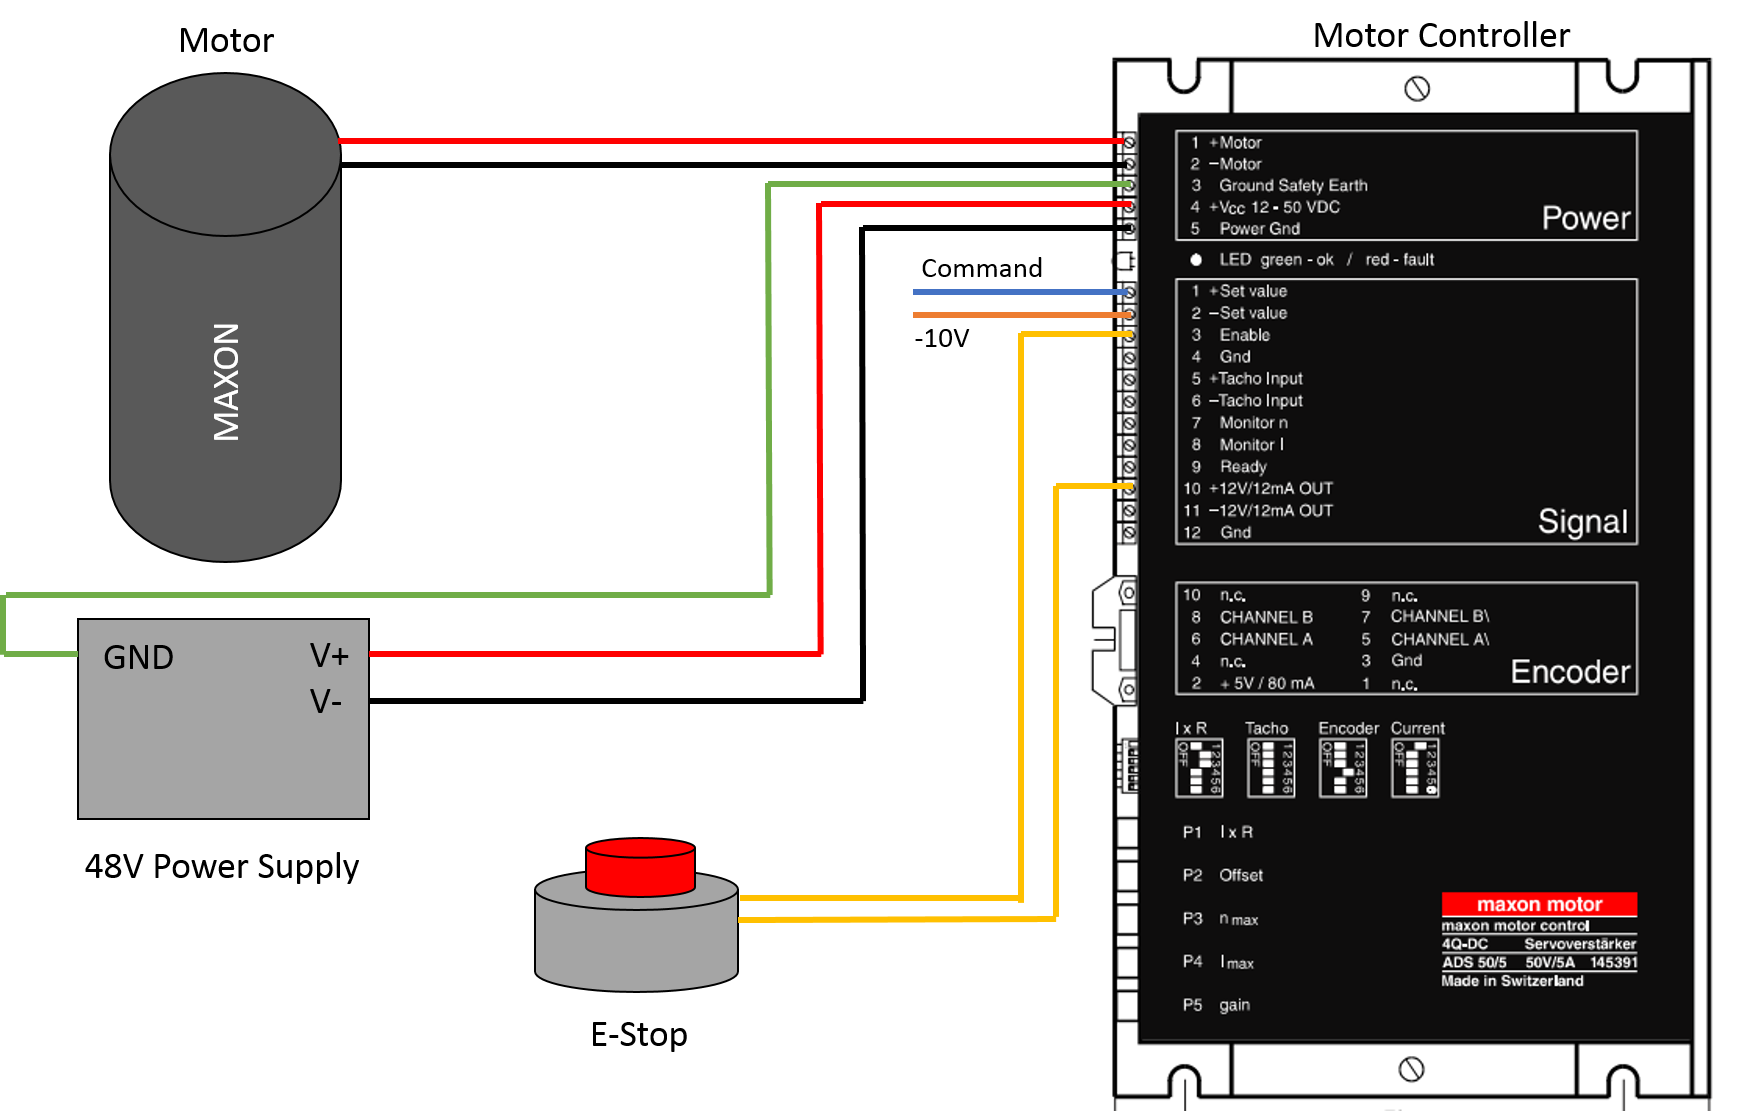
\includegraphics[width=0.9\linewidth]{Motor_setup}
		\caption{The belt drive and motor}
		\label{fig:actuator}
	\end{figure*}
		
	
	
	The PCB has four functions: supply power to the sensors, route signals to and from the DAQ, process or filter signals as necessary, and implement basic safety precautions. 
	\begin{itemize}
	\item \textbf{Power Distribution}: The entire device should run off of a single power supply so that only one wall outlet needs to be used. A 48V supply was chosen, since voltage is required by the motor. The sensors require 24V (Load Cell), and 5V (the IR sensor), and 10V is required to send commands to the motor controller. Therefore the PCB has three step-down voltage regulators at these three levels.
	\item \textbf{Signal Routing}: To streamline the wiring, the PCB takes in three main wires: a DB9 serial connection from the sensors on the footplate, a DB9 serial connection from  the power supply and motor controller, and a DB37 serial connection from the DAQ. These cables are connected to the PCB case and routed to the correct locations.
	\item \textbf{Signal Processing}: There are a few processing steps taken on the PCB (Fig. \ref{fig:amp}). An adjustable first order low pass filter is used to clean noise from the force measurements. The motor commands from the DAQ are also processed. The DAQ can output 0-5V from the analog pin, however the motor controller acceptc commands from -10 to 10V. The DAQ commands are amplified by 4 using a non-inverting amplifier implemented using an Op-Amp, such that the 0-5V output can be mapped to the +/- 10V input. 

	\begin{figure*}[h] 
		\centering
		
\includegraphics[width=0.4\linewidth]{ft_filter}
		
\includegraphics[width=0.4\linewidth]{amplifier}
		\caption{The command non-inverting amplifier and the force signal low pass filter}
		\label{fig:amp}
	\end{figure*}	
	
	\item \textbf{Safety}: The PCB implements four safety checks (Fig. \ref{fig:safety}). First, the motor commands is checked to ensure it is within an adjustable range. This range can be changed using potentiometers. A Watchdog timer is also used to ensure the software has not stalled. Every timestep, the software send a pulse to the timer -- if a pulse is missed within a certain delay, the Watchdog timer is triggered. There is also an emergency stop button which can be pressed at any time by operator or user. Th E-stop signal, Watchdog timer and motor command limits are combined in a logical AND gate, and the resulting output is sent to the enable pin on the motor controller. Any trigger from the three safety signals will disable the motor and stop the device.

	\begin{figure*}[h] 
		\centering
		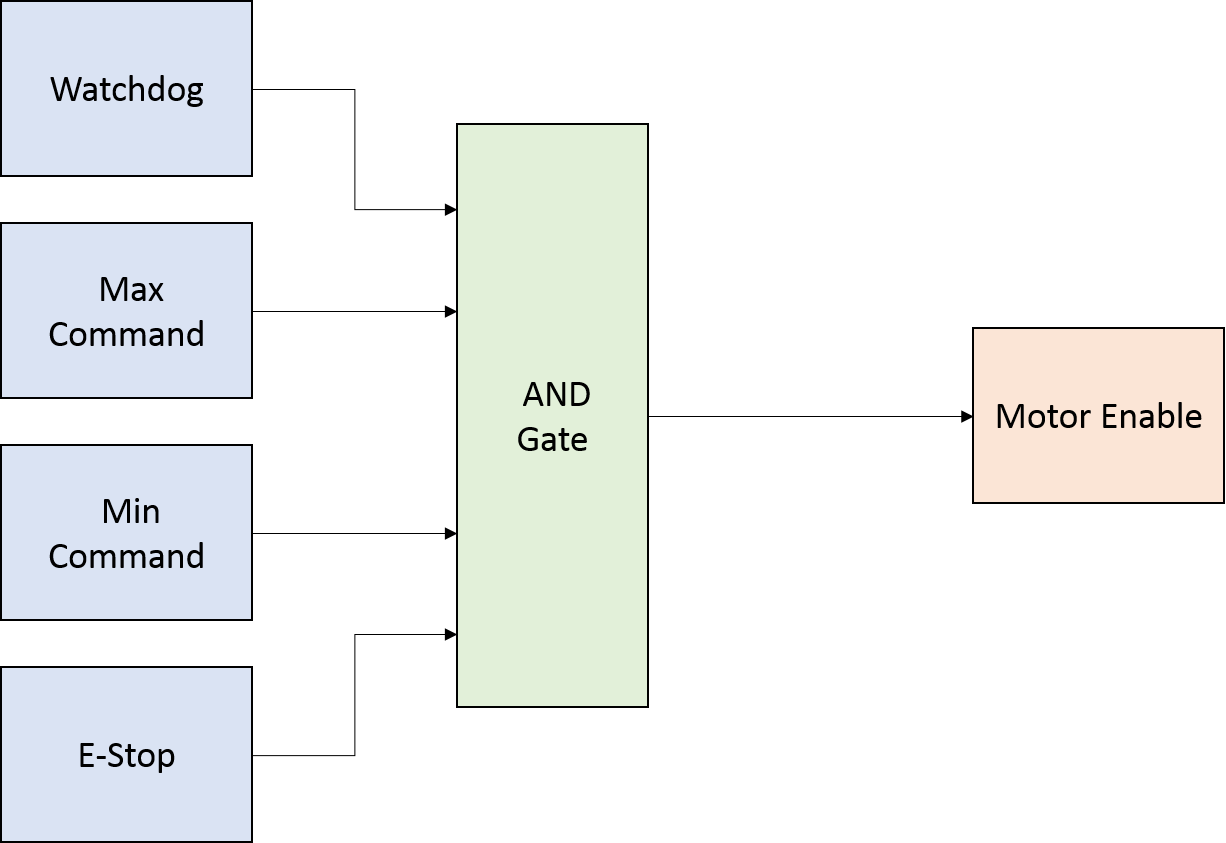
\includegraphics[width=0.6\linewidth]{electronics_safety}
		\caption{The safety system}
		\label{fig:safety}
	\end{figure*}	
	 
	\end{itemize}

		
		\subsection{PCB Layout}
		
		Originally, the electronics were mounted and routed on a prototype board, as shown in Fig. REF. The limited sized of the board was problematic, and the large number of jumper cables required to connect everything to the DAQ and to the other hardware made the setup disorganized, and difficult to troubleshoot. The design was streamlined by creating a custom printed circuit board (PCB), shown in Fig. . The layout was designed in Autodesk Eagle, and the board was manufactured by JLCPB (\url{https://jlcpcb.com/}). The first benefit of this design is the size, which contains more components in a smaller space and so can easily be mounted on to the robot. The wiring is also cleaner, with header pins arranged to minimize to bundle related signals together (\textit{e.g.} all wires going to the DAQ are together on the same unit of pins). A case was 3D printed to contain the PCB and the load cell amplifier. Three serial cables connect to the case: one for the motor controller, one for the DAQ, and one for the load cell and other sensors. 
		


	\begin{figure*}[h] 
		\centering
		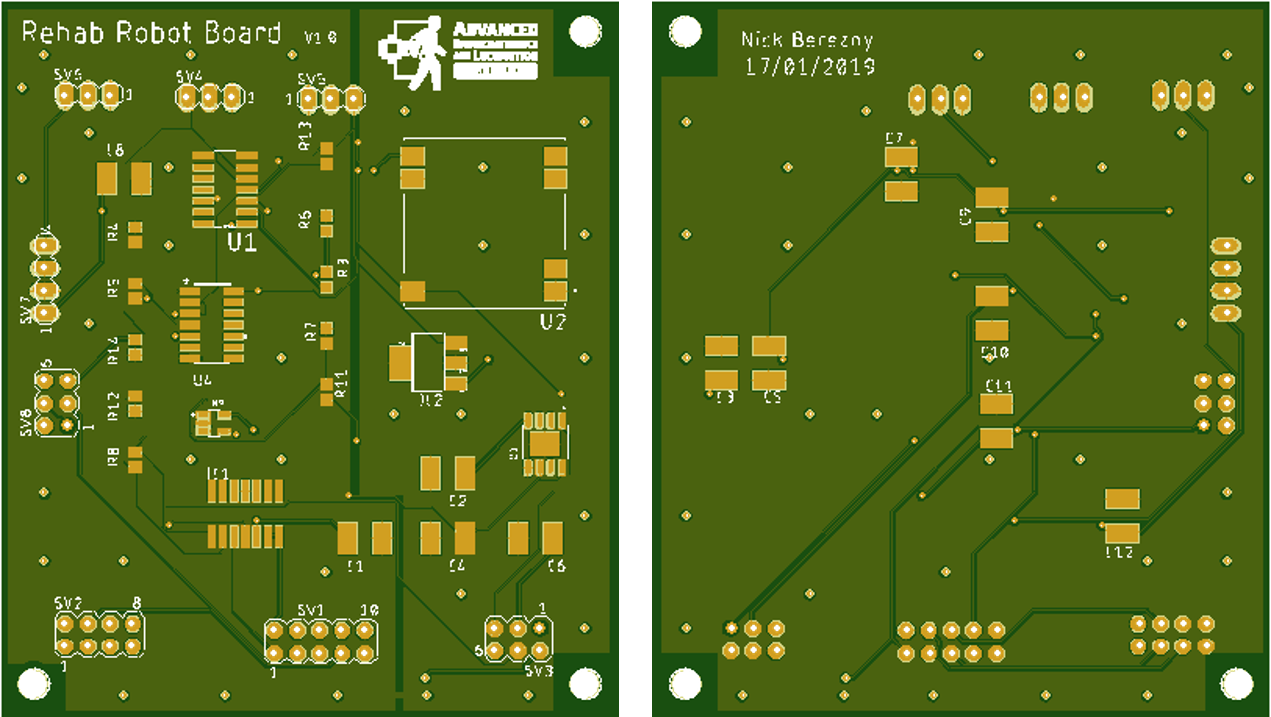
\includegraphics[width=0.75\linewidth]{pcb_pic}
		\caption{The PCB Layout}
		\label{fig:pcb_pic}
	\end{figure*}
	
		\begin{figure*}[h] 
		\centering
		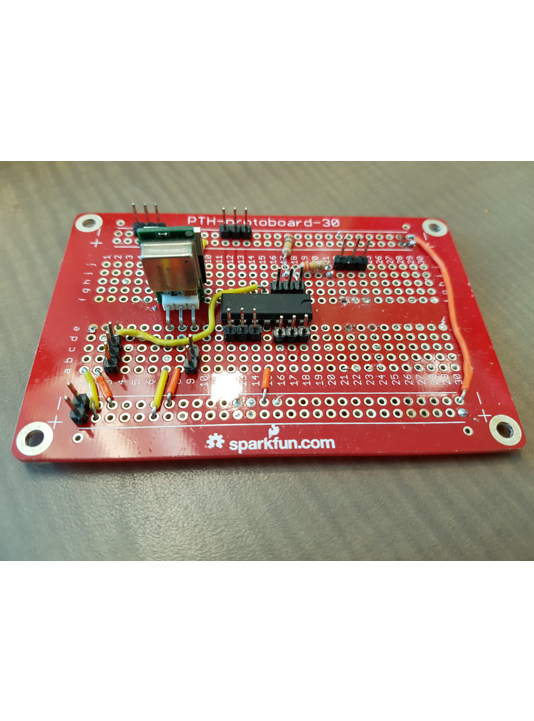
\includegraphics[width=0.4\linewidth]{protoboard}
		\: \:
		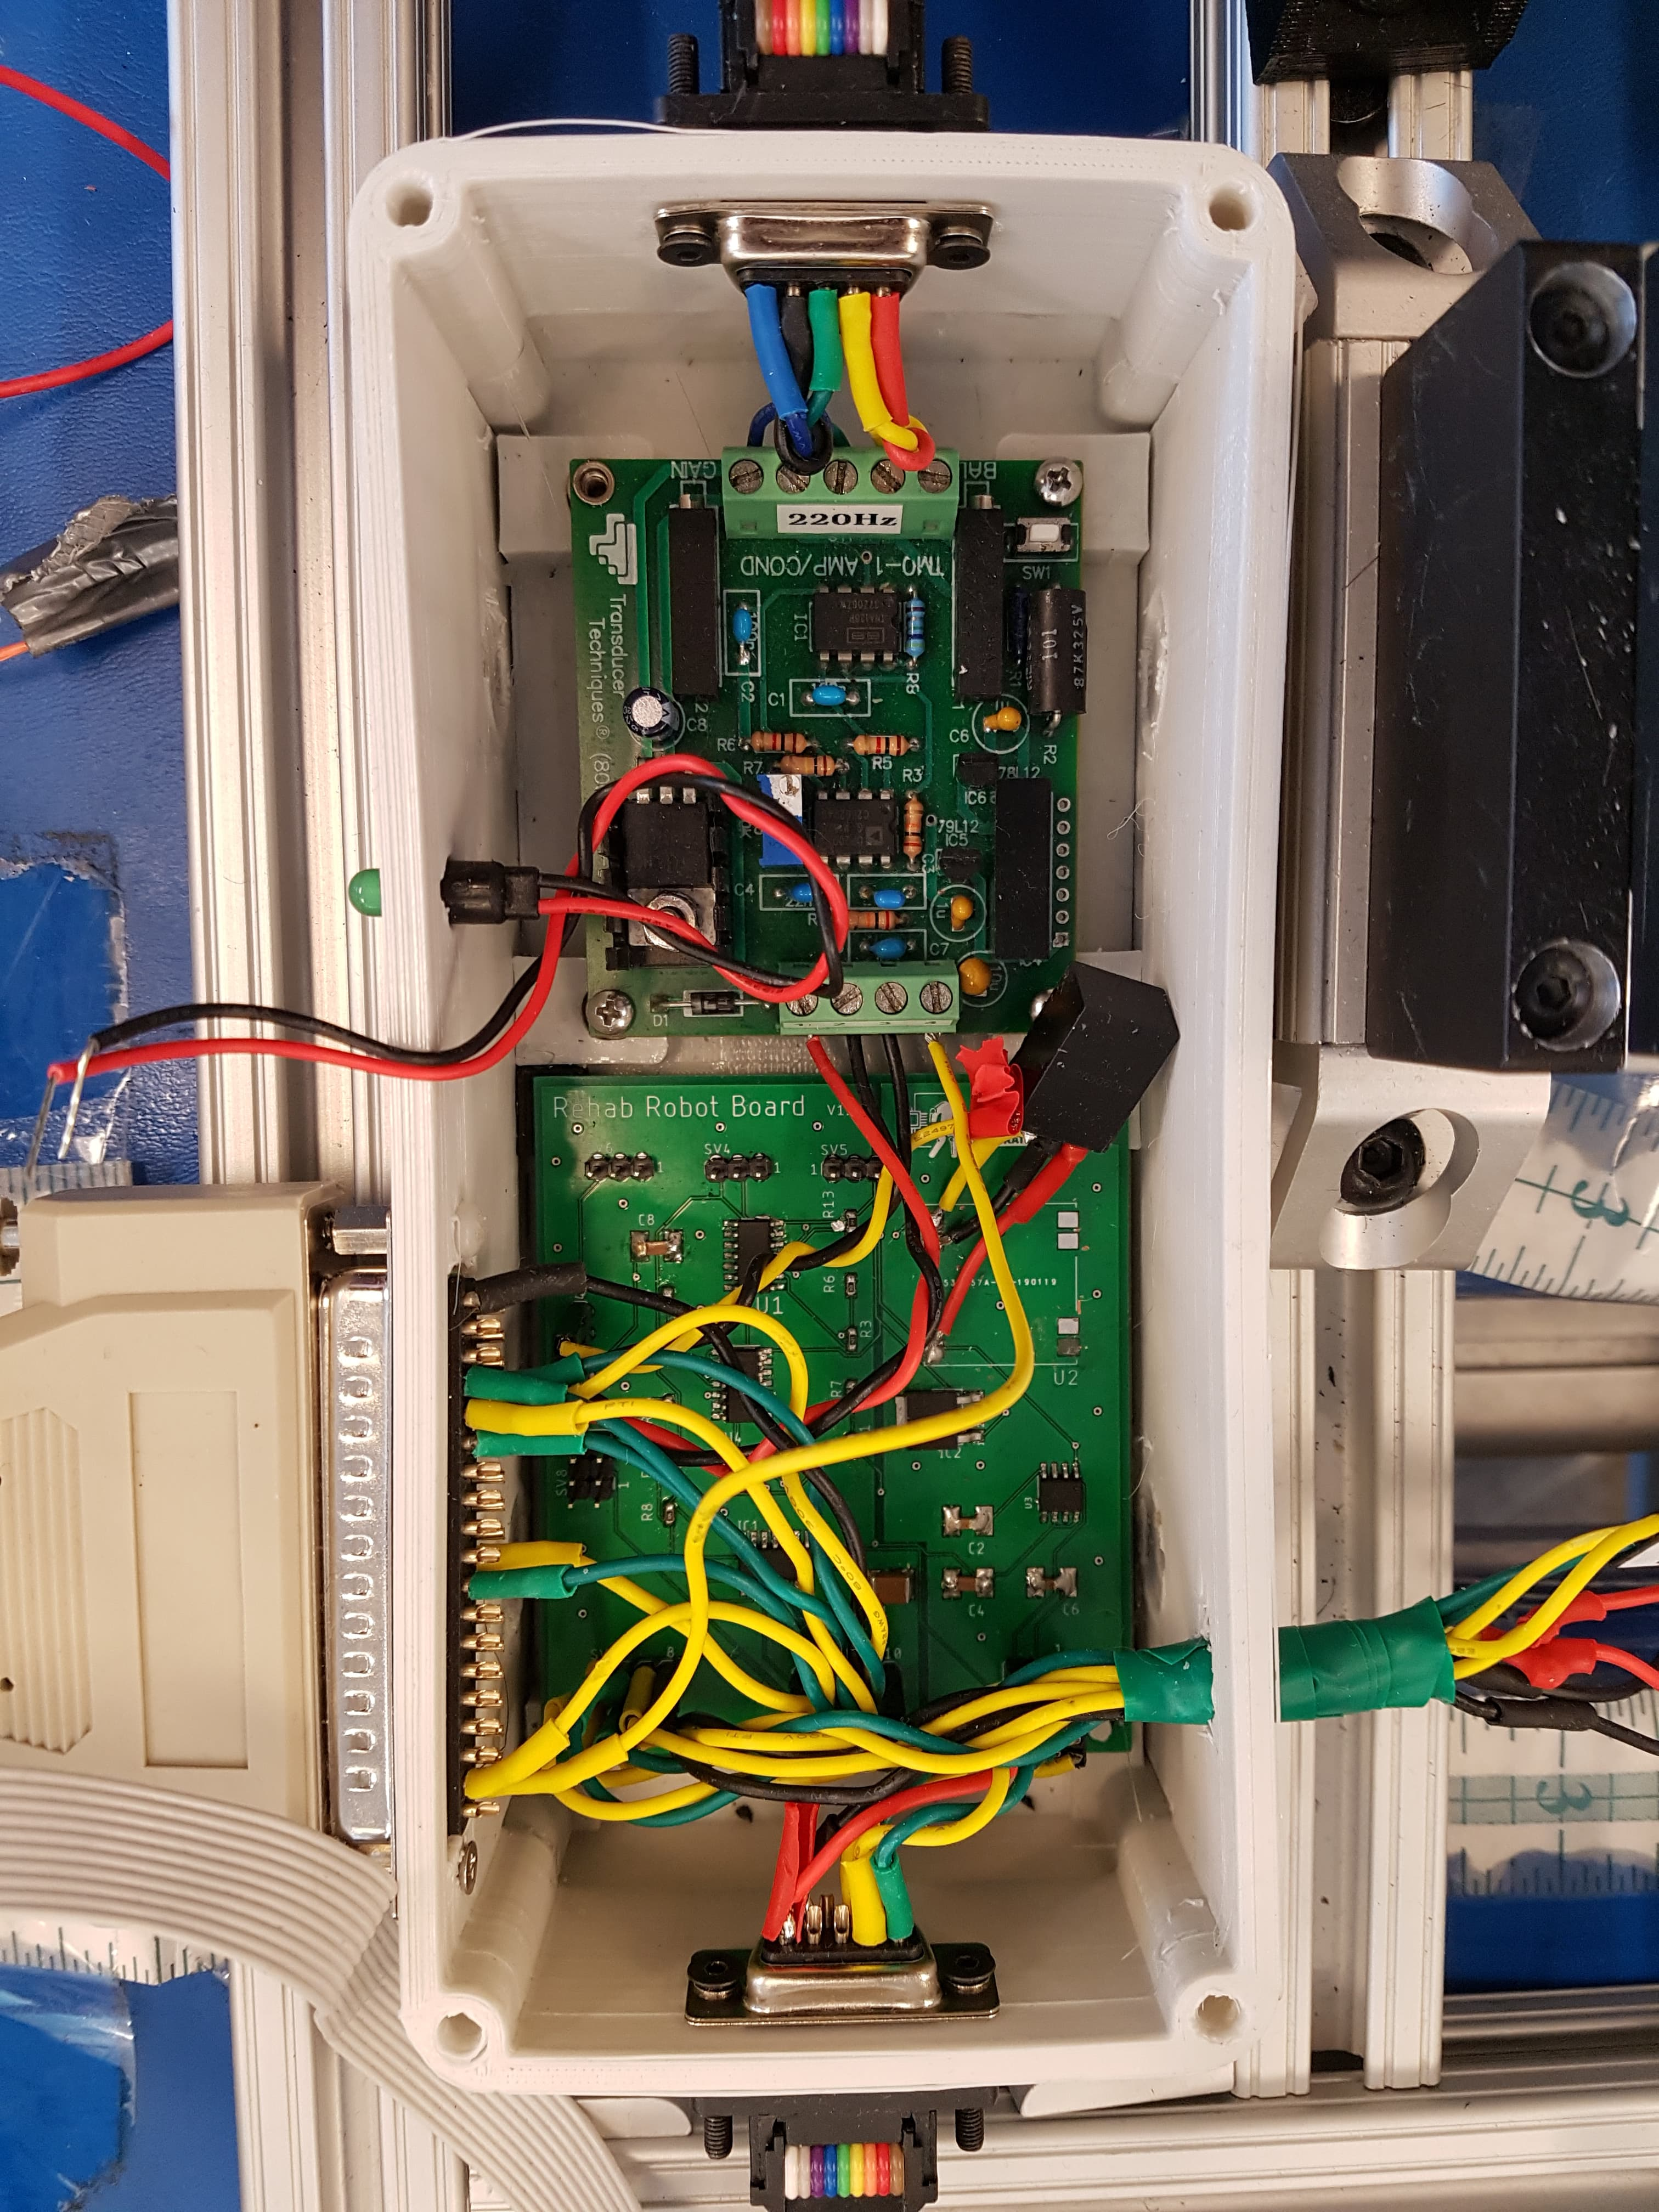
\includegraphics[width=0.4\linewidth]{pcb_case}
		\caption{The original protoboard (left), and the updated pcb and case (right)}
		\label{fig:robot_leg}
	\end{figure*}
	

	
	\section{Data Acquisition} 

	Data acquisition is handled by a LabJack T7 DAQ. This model has 14 analog inputs, 2 analog outputs, 23 digital I/O's, and is also capable of handling quadrature encoder signals and high-speed data streaming. The device can interface with the computer through a Ethernet, USB, or wifi (Ethernet was chosen for this project as it is the fastest and most reliable). The front-end Modbus TCP interface is conveniently packaged in the C/C++ LJM library, discussed further in chapter \label{ch3}.


	\section{Computer System}

	The control software and UI are run from an Intel NUC computer, with specification listed in Table \ref{tab:comp}. The computer's OS is Ubuntu VER. A wifi router is used to create a local network so that the UI can be accessed wirelessly. The DAQ connects to the computer via the Ethernet port. The system is shown in Fig. \ref{fig:comp}. 
	

	\begin{table}[h]
	\centering
	\caption{Computer Specifications}	
	\begin{tabular}{|c|l|}
		\hline
		Processor & 2.2 GHz Intel Core i5 \\ \hline
		RAM & 8GB DDR4 \\ \hline
		Memory & 250GB Solid State \\ \hline
		\end{tabular}
	\label{tab:comp}
	\end{table}
	

	\begin{figure*}[h] 
		\centering
		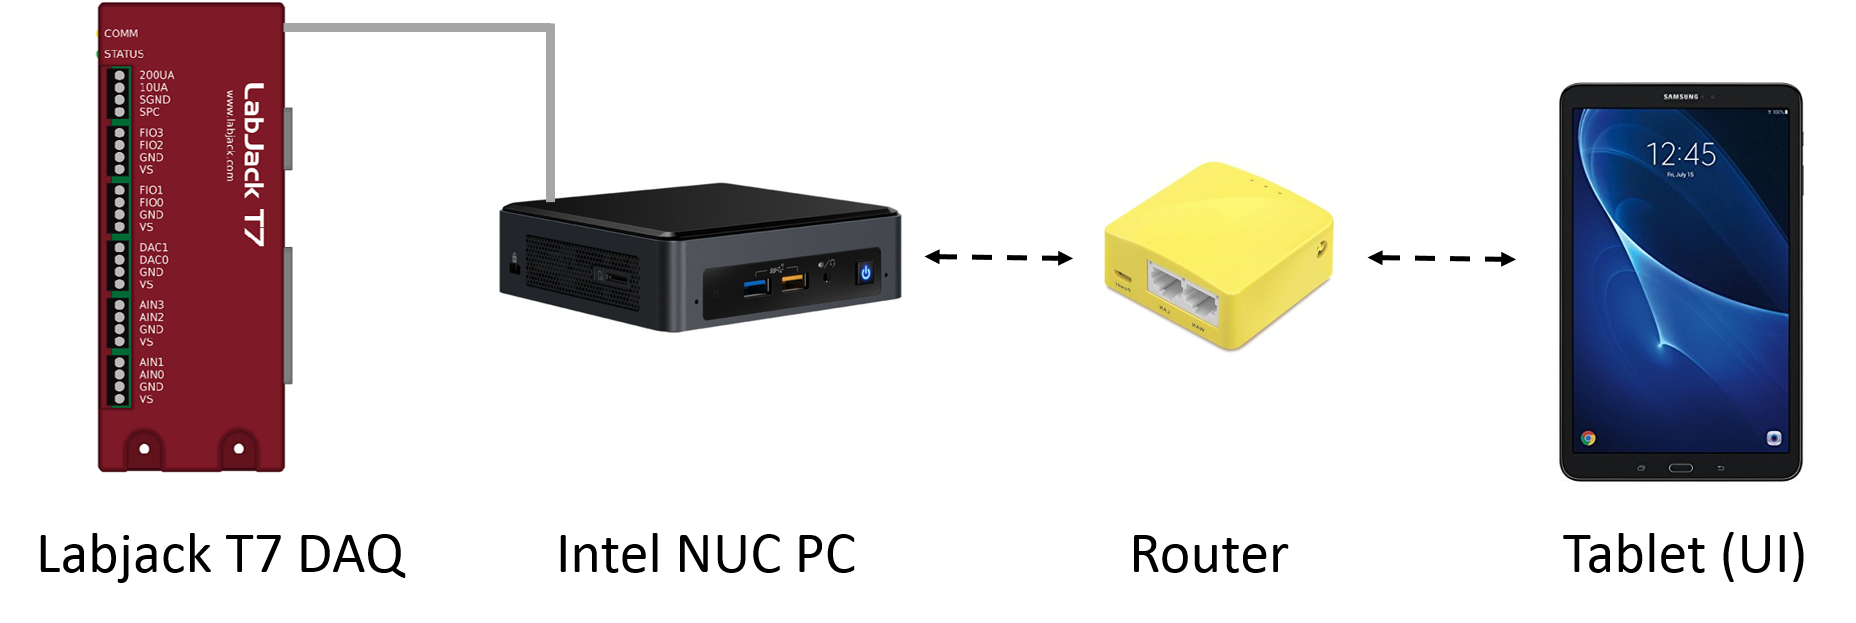
\includegraphics[width=0.75\linewidth]{computer_system}
		\caption{The Computer System, with DAQ, Router, and Tablet}
		\label{fig:comp}
	\end{figure*}
	
	
		
\chapter{Controller and Software} \label{ch3}


	\section{Overview}
	
	The controller and software must allow the device to perform the required tasks as laid out in chapter \ref{ch2}. This includes providing assistance to the patient through the exercise, but not to the extent that the patient can become passive and allow the robot to drive the motion. The level of assistance should be adjustable so that the operator can tailor the session to the capabilities of the patient. The software must also engage the patient using virtual environments and games. These must be related to the motion of the exercise, such that the robot becomes a control input into the game, and the patient is rewarded for following the desired trajectory. Immersion within the virtual environment could also be bolstered by haptic feedback, or the physical rendering of virtual forces to the patient through the robotic device. 
	
	\begin{figure*}[h] 
		\centering
		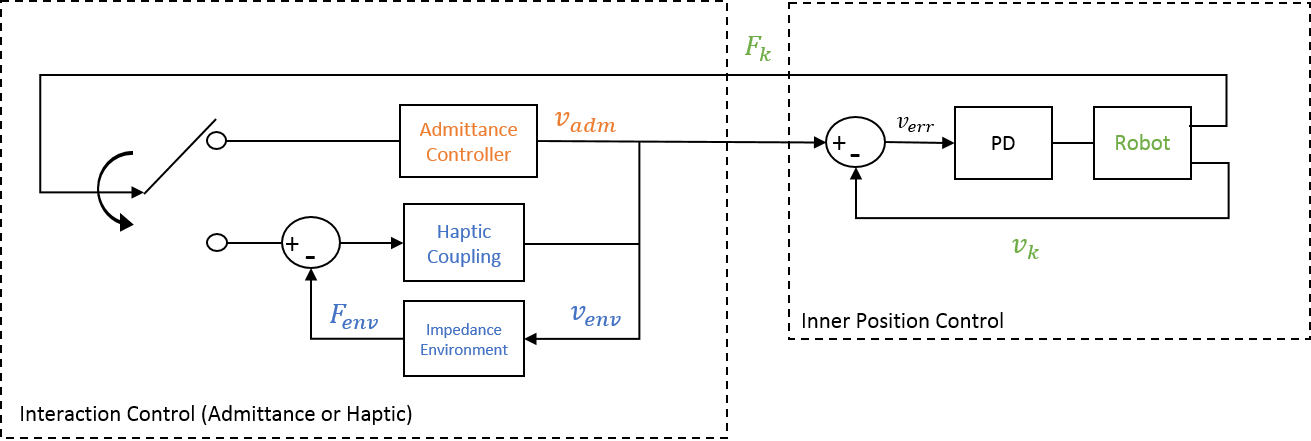
\includegraphics[width=\linewidth]{control_diagram2}
		\caption{Virtual Haptic Coupling for Admittance Control}
		\label{fig:software}
	\end{figure*} 
	
	\section{Impedance \& Admittance Controller} \label{Sec:imp}

%------------------------------------------------------------------------
%-Explain force control
%	-choice of impedance over admittance
%-Implementation in code
%
%-------------------------------------------------------------------------

Both position and force control may behave unpredictably when interacting with an unknown environment, and may not be well suited for the purposes of assisting patients through rehabilitation movements. Position control would not provide assistance as needed, but would simply force the user's leg through the motion, similar to a passive motion machine. Force control is not sufficient since it does not allow the controller to follow a predefined trajectory. Interaction control, also known as impedance/admittance control, was introduced in \cite{Hogan1985}. Instead of controlling position or force directly, interaction control seeks to control the dynamic relation between the position and force variables. 
	
There are two possible causalities -- an impedance, which accepts a velocity/position and renders a force, and an admittance, which accepts force and renders a velocity/position. An interaction controller will chose one of these causalities, and will sense input from the physical device, calculate the output variables based on some virtual desired system, and then command the device to that output. A commonly used virtual system is the mass-spring-damper system shown in Fig. \ref{fig:mass-spring-damper}. 

	\begin{figure*}[h] 
		\centering
		
\includegraphics[width=0.75\linewidth]{admittance_sys}
		\caption{A mass-spring-damper system, with the origin of the spring set to some desired trajectory}
		\label{fig:mass-spring-damper}
	\end{figure*}
	
Impedance control measures the position and velocity of the robot, and then calculates the force generated by the virtual system, as in Eqn. \ref{eqn:imp} \& \ref{eqn:imp_msd}. The device must then use force control to achieve the desired output force, which is usually done by computed-torque methods. 

\begin{equation} \label{eqn:imp}
	F = ZV_R 
\end{equation}  

\begin{equation} \label{eqn:imp_msd}
	F = m\ddot{x} + b\dot{x} + k(x - x_{des})
\end{equation} 

Using this control law, the end effector of the robot will behave like the system above, about point $x_{des}$, when displaced by the external environment. If, for example, an operator physical moved the robot, it would respond as if it were the mass-spring-damper system, \textit{i.e.} it would apply a resistive force related to the extent to which it was displaced. 
	This control law rests on a significant assumption -- that the robot itself has no inherent impedance between the actuator and the the end-effector. It is possible to cancel some of the impedance of the robot using ..., however this is less common and generally takes more time and is less successful (ref). This is an idealization - there will also be some level of friction, mass, or other impeding factors in the motor, gears, links, etc. Therefore, impedance control should only be considered for robots made of low impedance components, such as belt drives and direct-drives. 
	
	\begin{figure*}[h] 
		\centering
		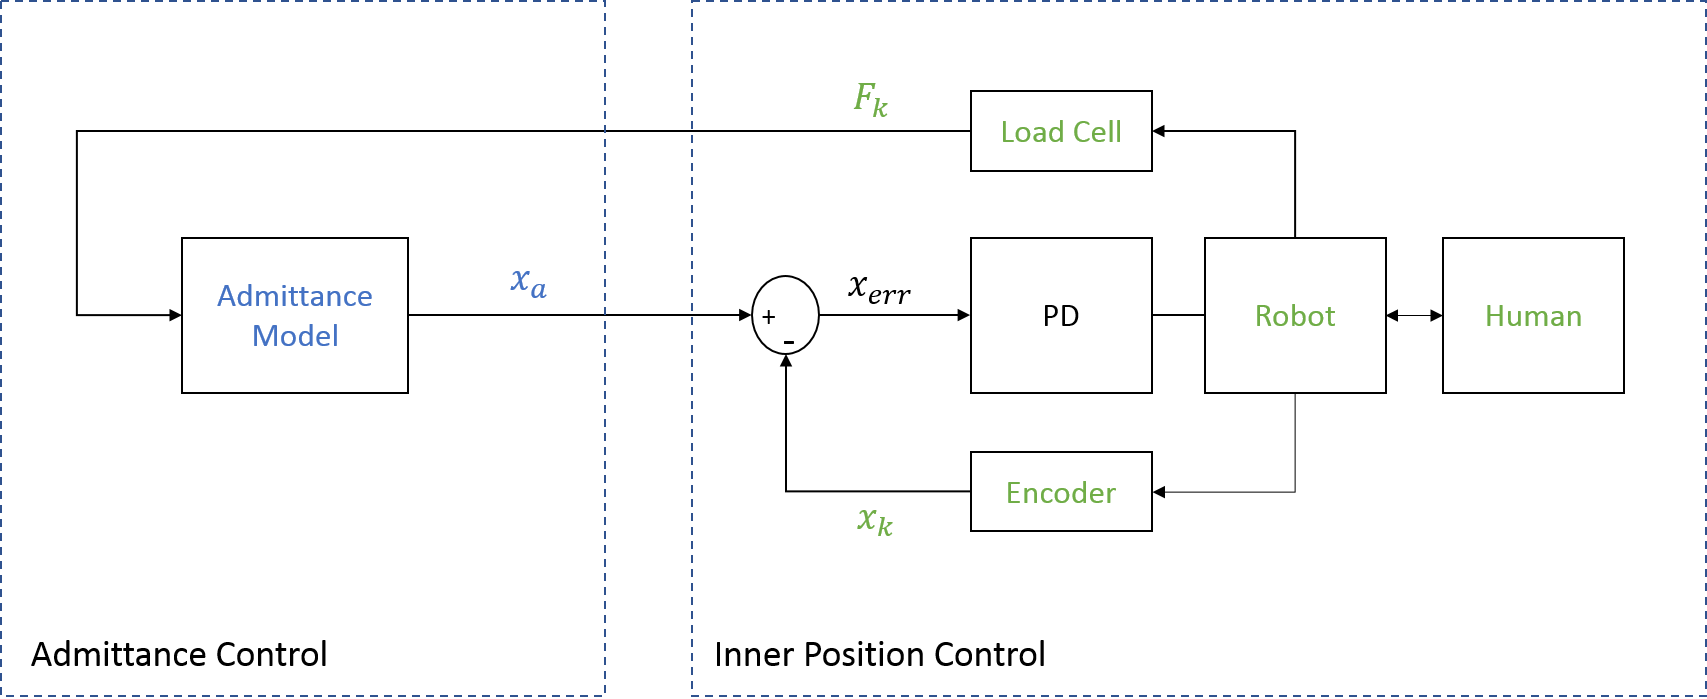
\includegraphics[width=0.65\linewidth]{admittance_diagram}
		\caption{Admittance control flow chart}
		\label{fig:adm_diagram}
	\end{figure*}
	
	Admittance control is essentially the inverse of impedance control, in that it accepts an external force and then renders a corresponding displacement. Fundamentally, admittance control can be described by the following equation, where $F_R$ is the force applied to the robot, $Y$ is the desired admittance, and $V$ is the 'flow' variable vectors (e.g. position and velocity) :
	
	\begin{equation}
	V = YF_R 
	\end{equation} 
	
	Once again, it is common to define admittance in terms of a mass-spring-damper system (\ref{eqn:adm}). Here, $x_a$ and $v_a$ are the ``simulated'' position and velocity determined by the admittance controller. Additionally, to actually render the desired position and velocity, an outer-loop PD position controller is used (\ref{eqn:PD}), with $x_a$ and $v_a$ acting as the desired position and velocity. 
	
	\begin{gather} \label{eqn:adm}
	\begin{bmatrix}
    	\dot{x}_a \\
    	\dot{v}_a 
    \end{bmatrix} 
    =
    \begin{bmatrix}
    	0 & 1 \\
    	\frac{k}{m} & \frac{b}{m}
    \end{bmatrix} 
    \begin{bmatrix}
    	x_a \\
    	v_a
    \end{bmatrix}  
    +
    \begin{bmatrix}
    	0 \\
    	\frac{1}{m}
    \end{bmatrix}
    F_R   	
	\end{gather}
	
	\begin{equation} \label{eqn:PD}
	F = P(x - x_a) + D(v - v_a)
	\end{equation}

	Admittance control assumes that the robot has infinite impedance, or that all hardware between the actuator and the end-effector is infinitely stiff, infinitely damped, etc. This, once again, is an idealization -- and therefore admittance control should only be considered when the robot has high impedance, i.e. when using large gear reductions and rigid links. 
	
	Another point of consideration when choosing between impedance and admittance control is its stability when encountering different types of environments. Impedance control works better when interacting with an admittance (rigid environments), whereas admittance control works better when interacting with an impedance (weak environment / free space). This project targets acute stroke patients who typically do not have much leg strength and rely heavily on assistance from the therapist during therapy. Therefore, these patients can be modeled as an impedance. Furthermore, the motor used on the robot has a high gear reduction which contains substantial impedance. Both of these favour using admittance control. 
	
	Admittance control is implemented by taking the Z-transform of Eqn. \ref{eqn:adm}, updating the desired position based on these discrete step equations, and then using PD controller to move to this desired position. ...
	
	The linear admittance control system in Eqn. \ref{eqn:lin_sys} is discretized according to the Eqn. \ref{eqn:Ad} \& \ref{eqn:Bd}.
	
	\begin{equation} \label{eqn:lin_sys} 
	\dot{X} = AX + BF
	\end{equation}
	\begin{equation} \label{eqn:Ad} 
	A_d = e^{At} 
	\end{equation}
	\begin{equation} \label{eqn:Bd} 
	B_d = A^{-1}(A_d - I)B
	\end{equation}
	
	\subsection{Velocity Profile}	
	
	The final step is to set the desired position a suitable trajectory. The system is 1-DOF, so this can be done simply by creating a velocity profile. The velocity profile is defined in terms of the total length of the linear stroke ($x_{max}$) as well as the maximum velocity that we want to have at any point ($v_{max}$). At first, a quadratic relation was used, creating a parabola with zero velocity at each endpoint and $v_{max}$ in the center. This was found to feel unnatural. The final profile is shown in Fig. \ref{fig:velocity_profile}, with constant acceleration to $v_{max}$, a plateau of constant velocity, followed by a constant deceleration. The same profile is inverted to move back at the end of the stroke. The transition points were set empirically, with acceleration up to $0.4 x_{max}$, and deceleration beginning at $0.6 x_{max}$. 
	
	\begin{figure*}[h] 
		\centering
		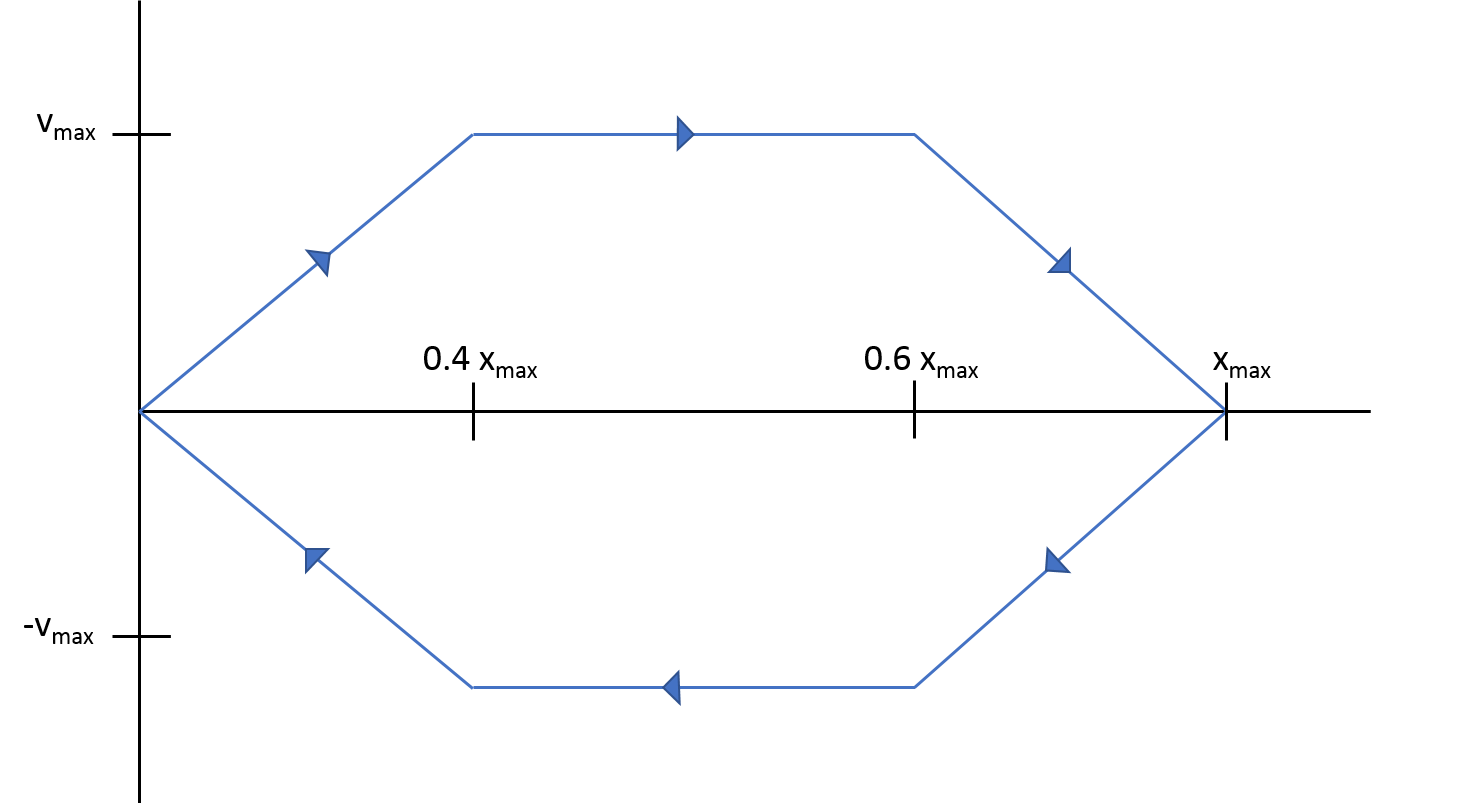
\includegraphics[width=0.75\linewidth]{velocity_profile}
		\caption{Velocity Profile of the Desired Trajectory}
		\label{fig:velocity_profile}
	\end{figure*}
	
	
	
	\subsection{Operational Modes Using Admittance Control}
	
	Two operational modes use the admittance control with the mass-spring-damper system -- trajectory tracking with assistance, and trajectory tracking with resistance. 
	
	\textbf{Trajectory Tracking with Assistance}: The mass-spring-damper system is used with a moving spring origin set to the trajectory as defined by the velocity profile. The spring stiffness represents the level of assistance, with stiffer springs providing more assistive force. The assistance is low when the error is low, therefore only providing assistance as needed. 
	
	\textbf{Trajectory Tracking with Resistance}: The spring term is omitted (\textit{i.e.} k = 0.0) so that the user only feels damping and mass. The damper term now represents viscous resistance, with higher damping parameters creating greater resistance. Without the spring term, there are no assistive forces and so the patient must provide all motion on their own. This mode could be used for more capable patient's who need a challenge, or for strength building. 
	
	

	\section{Haptic Coupling} \label{sec:haptic}
%------------------------------------------------------------------------
%-1 DOF physics engine 
%-strategies to create haptics 
%	-changing imp params
%	-virtual coupling
%
%-------------------------------------------------------------------------

Defining the desired impedance or admittance in terms of a mass-spring-damper system is not always convenient. Ideally, one could define an arbitrary impedance or admittance function relating $F$ and $V$, giving complete control of the behaviour of the robot-environment interaction, while also ensuring stability. The dual goals of imposing a 
	
	A method for achieving arbitrary interaction and remaining stable is discussed in \cite{Adams1999}, using what is called a ``haptic coupling''. This effectively decouples the design on the admittance/impedance and analysis of the stability of the robot. Consider again the two-port model of the robot-environment interaction. The haptic coupling is a virtual passive system placed in between the two, which acts as a low pass filter on the variables. This limits the range of renderable impedances, and while it does alter the desired impedance to some extent, the trade off is guaranteed stability. Using the concept of the haptic coupling, a simple physics engine was designed which works in conjunction with the games and visualization.
	
	\begin{figure*}[h] 
		\centering
		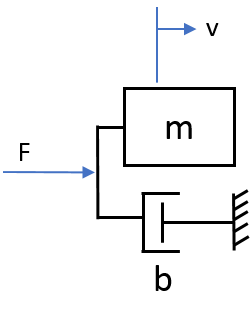
\includegraphics[width=0.3\linewidth]{haptic_coupling}
		\caption{Virtual Haptic Coupling for Admittance Control}
		\label{fig:haptic_coupling}
	\end{figure*} 
	
	\begin{figure*}[h] 
		\centering
		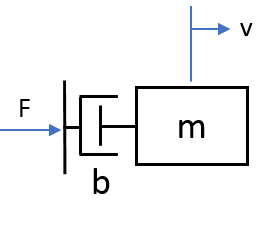
\includegraphics[width=0.3\linewidth]{haptic_coupling_original}
		\caption{Virtual Haptic Coupling for Admittance Control}
		\label{fig:haptic_coupling_original}
	\end{figure*} 
	
	In addition to decoupling stability and the design of the haptic environment, the haptic coupling also allows both impedance and admittance to be used together. For example, a robot may use admittance control due to large amounts of drive friction, but the haptic environment may need to be defined as an impedance, \textit{i.e.} using position to calculate the desired haptic force. 
	
	\begin{equation}
		Z(s) = \frac{F}{v} = ms + b  
	\end{equation}
	\begin{equation}
		Z(z) = \frac{mb(z-1)}{(m+bT)z - m}
	\end{equation}
	
	The z-transform yields the control step algorithm in Eqn. \ref{eqn:ztrans}. These are used to calculate the present time environmental position/velocity. 

\begin{equation} \label{eqn:ztrans}
	v_k = \frac{m}{T}v_{k-1} + \frac{f_{k-1} - f}{\frac{m}{T} + b}
\end{equation}
\begin{equation}
	x_k = x_{k-1} + v_{k}T
\end{equation}

	
The underlying virtual physics should have an impedance causality, and so the environmental force is calculated based on this position/velocity pair. This mapping can be an arbitrary function, thanks to the haptic coupling (Eqn. \ref{eqn:imp}). 
 
\begin{equation} \label{eqn:imp}
	f_k = \mathcal{F}(x_k, v_k)
\end{equation}

For example, to achieve the standard admittance control from the previous section, the impedance mapping can generate the spring component (with the damping and mass contributed by the haptic coupling), as in Eqn. \ref{eqn:spring}

\begin{equation} \label{eqn:spring} 
	f_k = K(x_k - x_{des})
\end{equation}

With the haptic coupling, more complex environments can be created. For example, contact between the user and a virtual object can be rendered. The interaction force is set to zero when there is no contact, allowing for free motion. When in contact, the interaction force can be modelled a number of ways, including with a simple spring

\begin{equation}
$$
\[ 
f_k = 
     \begin{cases}
       \text{no contact} &\quad f_k = 0 \\
       \text{contact} &\quad f_k = k(x_{user} - x_{dist}) \\
     \end{cases}
\]
$$
\end{equation}

\subsection{Operational Modes Using the Haptic Coupling}

Only a single mode is implemented using the haptic coupling -- a simple interactive balance game. The player is tasked with maintaining a static position within a small margin of error. Disturbances are launched at the player from both directions, which contact the user and produce a haptic force 

\subsection{Physics Engine}
	
There physics involves the movement of two objects, the character and the disturbance, as well as the interaction force between them. There are three cases:

\begin{enumerate}
	\item Disturbance is out of play: The disturbance has left the environment. A new one is randomly spawned to either the right or left of the environment, and given a fixed initial velocity.
	\item No Contact: There is no contact. The position of each object is updated, with the character's position set equal to the position of the device, and the disturbances position set according to its constant velocity. 
	\item Contact: The character's sphere overlaps the disturbances sphere, and are therefore in contact. The contact force is modelled a linear spring, with the distance between the objects' centres times the contact stiffness equal to the interaction force. 
\end{enumerate}

	
	\section{Tuning Control Gains}

	Some control gains must tuned for optimal performance and stability, which include:
	
	\begin{enumerate}
		\item P \& D for the position PD controller 
		\item b \& m for the haptic coupling ()
		\item $I_{max}$ on the motor controller, giving the current command given to the motor at the maximum motor command of $\pm 10V$
	\end{enumerate}		
	
	Other controller gains are set based on the desired behaviour of the device -- these require bounds so that the user does not enter bad parameters:
	
	\begin{enumerate}
		\item K,B,M for the admittance controller
		\item $V_{max}$ for trajectory generation
		\item $F_{max}$ for the maximum force generated by the system
	\end{enumerate}
	
	...
	
	First, the PD controller can be tuned separately from the admittance. The PD controller can be though of as another impedance existing within the system, and should therefore be tuned as high (stiff) as possible for optimal performance of the admittance controller. The P gain should be set such that the largest position error corresponds with the maximum motor command.
	
	The maximum motor command at the motor controller is $\pm 10V$, however the motor command sent from the DAQ is multiplied by a factor of approximately 4 and referenced to a constant $10 V$. Therefore the maximum command sent from the controller is between 0 (maximum current in one direction) to 5 (maximum current in the other direction). 
	
	The maximum displacement can be calculated by using the maximum velocity achievable by the actuator. In this case that is $9 in/s$, which corresponds to a maximum displacement of about $0.23 mm/step$ for a controller running at 1000 Hz. However, designing for this displacement will be conservative in that the gains will be very small. Furthermore, since the system is interacting with a person whose behaviour is unknown, there is always the chance the system will be driven beyond the limits. Therefore it was decided to design the PD controller based on a maximum step of 2mm, and to then try and enforce the maximum velocity of $9 in/s$ through visual feedback to the user.
	
	Given these parameters, the P gain should be set to 2.4:
	
	\begin{align*}
		cmd_{max} &= P\Delta x \\
		P &= \frac{cmd_{max}}{\Delta x} = \frac{4.8}{2} =  2.4
	\end{align*}
	
	Next, the D gain is determined empirically by increasing it until there is no overshoot to a step response ....
	
	The limits on the admittance parameters can now be determined. The admittance system can be approximated by the following:
	
	\begin{equation}
		\Delta v = - \frac{K}{M}x - \frac{B}{M} + \frac{1}{M}F
	\end{equation}
	
	We want to avoid producing a change in position greater than 2mm as per the PD controller tuning. Therefore, the maximum velocity of the admittance model should not exceed 2000 mm/s (for a controller running at 1 kHz). Therefore, $\Delta v$ should be equal to zero at this maximum velocity and at the maximum achievable spring force, \textit{i.e.} when the error between actual position and reference position is maximum. Therefore:
	
	\begin{align}
		0 &= -K(400mm) - B(2000mm/s) + 222.4N \\
		K &\leq 0.556 - 5B   
	\end{align}
	
	he mass is factored out, and the maximum error in position, maximum velocity, and the maximum force are entered. This defines space bounded by a line in which the $(K,B)$ vector must lie. Furthermore, there is a minimum constraint on the damping (B) since it is the dissipative element and is therefore required for passivity and stability. This constraint, $B_{min}$ is found empirically by setting K high and finding the minimum B to make the system behave in a stable manner. ...

	The mass does not affect the rendered impedance, but instead determines the systems sensitivity to force. The smaller the mass, the smaller the force that is required to achieve a certain state ... There is therefore no real maximum mass, however at some point a high mass will make the system impossible to move. There is a minimum mass, below which the sensitivity to force allows sensor noise or unmodeled dynamics to effect the system to an undesirable extent. 
	
	...
	
	Finally, the haptic coupling parameters $m$ and $b$ should be set. As was explained in Sec. , these parameters give the controller some minimum impedance so that the haptics do not try to render an impedance too close to free motion. Therefore, the parameters are set to the empirically derived $B_{min}$ and its pair $K_{min}$. This decouples the haptic design from the stability of the controller by imposing the minimum impedance for the stability. The maximum constraints are however still not imposed. Fortunately, the haptics explicitly calculate either the desired force or the desired next position, and therefore the constraints on these parameters can be directly imposed. 
		

	
			
	\section{Software}	

	The controller needs to be implemented in software, along with communication, data logging, and a User Interface for setting up and displaying visuals. The software is split into two parts: the control software and the user interface software. The entire codebase is available on GitHub at \href{https://github.com/nickberezny/RehabRobot}{https://github.com/nickberezny/RehabRobot}. It is built to run on real time enabled Linux, and should run on any hardware (assuming it has sufficient memory and RAM, and an ethernet port to connect with the DAQ). This modularity should make it easy to use this code in future iterations of the project which may use different hardware. To date, it has been tested on the Intel NUC used in this project, as well as on a Raspberry Pi 3B. 
	

	

	\subsection{Real Time Operation and Linux}
	
%------------------------------------------------------------------------
%-Explain Real time
%	-features
%-Explain Linux Real time
%	-POSIX
%-Details of robot software (threads, libraries, memory ...)
%	-threads, memory sharing 
%
%-------------------------------------------------------------------------

A real time system is one in which the timing of the computations significantly affects the results \cite{Lewine1991} --  in other words, a missed computational deadline can be detrimental to the performance of the system. Systems can either be soft real time or hard real time, a distinction made based on the danger associated with missing a deadline. Hard real time system will cause serious harm or damage if a deadline is missed (\textit{e.g.} the control systems on a Jet), while the consequences are typically minor in soft real time systems. The distinction can be vague, but in general hard real time systems require programs which are mathematically proven to be real time (REF), whereas soft real time systems can get away with less stringent requirements. 

The consequences of a missed deadline in our system is at worst sending the wrong motor torque command to the actuator, which in the absolute worst case scenario will cause the maximum torque command to be issued. However, motor torque commands are limited for safety (see sec...), and the operator and user have access to an emergency stop. Therefore, we deemed that the system requires only soft real time capabilities. 

Linux is an operating system (OS) based on UNIX which is open source and comes in variety of versions or flavours, including Ubuntu. Linux can be used as a standard home computing operating system like Windows or Mac, and is also found commonly in embedded system where the OS is highly tailored to a specific set of hardware. (refs!). The Linux kernel is not inherently real time -- there is a patch available which adds soft real time capabilities to the OS. This is known as Real-time Linux or RTLinux, and is created using the Preempt RT patch \cite{SebastianSiewior2019}. The patch allows programmings to use the following real time functionalities, as defined in the real time standard extension of the original Portable Operating System Interface for Computing Environments (POSIX) \cite{Obenland}.

\begin{itemize}
	\item \textbf{Threads}: POSIX threads, or pthreads, are used for parallel computing. Multiple threads can run under a single process and share its memory space.
	\item \textbf{Priority Scheduling}: Allows setting thread priorities, with higher priority processes pre-empting lower priority processes. This helps critical control code to run uninterrupted by less important work. 
	\item \textbf{Mutexes}: A Mutual Exclusions Object is used to orchestrate data sharing between threads. Once one thread takes ownership of a Mutex, others cannot access it before it is unlocked. This prevent other threads from changing the data before the previous thread is finished. 
	\item \textbf{Memory Locking}: Locks memory into RAM to prevent the program from accessing the hard disk (Page Faults), which can cause delays. 
\end{itemize}
	
	\subsection{Controller}
	
	The controller is written in C, and is designed to achieve low latency so that it can meet sampling rate deadlines. The target frequency is 1kHz, or 1ms per time step. The controller on average runs at 1.05 ms per time step, or approximately 9.5 kHz. More information of delays and jitter in the control software can be found in Sec REF... 
	
		\begin{figure*}[h] 
		\centering
		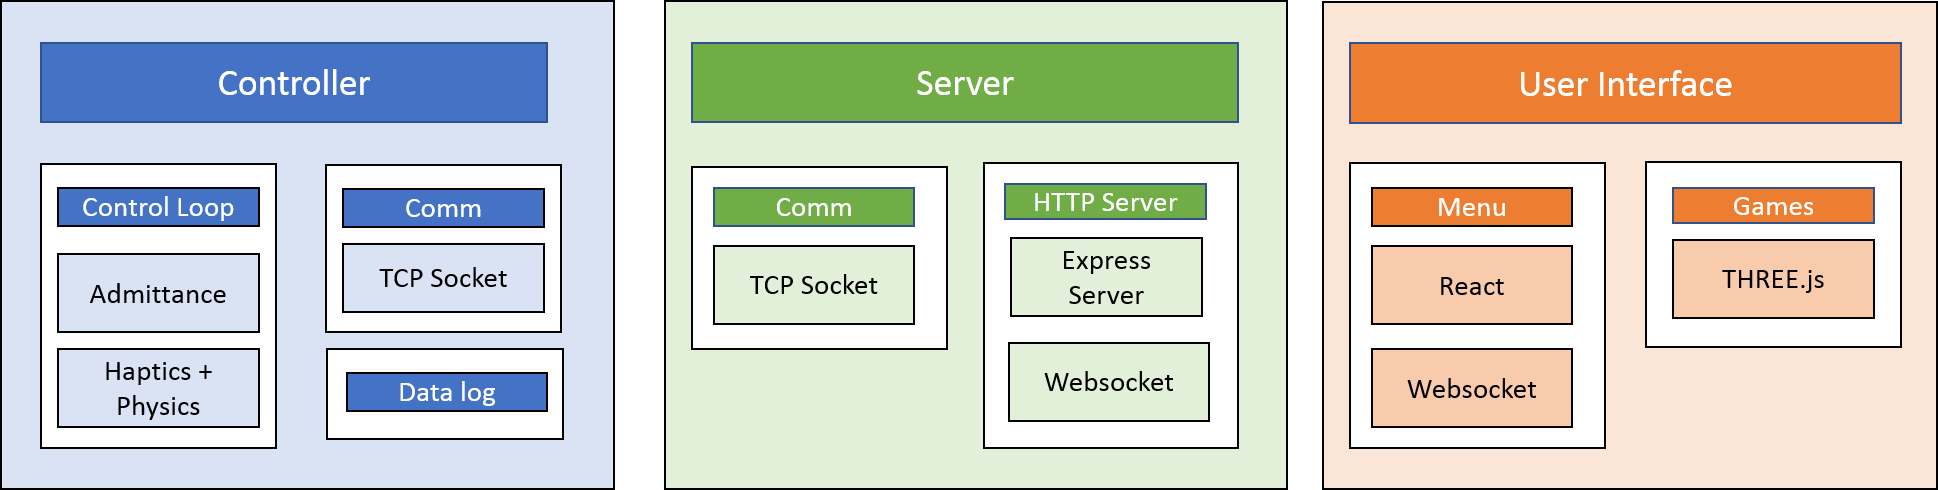
\includegraphics[width=\linewidth]{software}
		\caption{The Three Threads in the Control Software}
		\label{fig:software}
	\end{figure*} 
	
	
	The controller process is split into three threads: the controller, the server communication, and data logging, with priority levels of 98, 97, and 96 respectively. The controller has highest priority and can pre-empt the others to keep it running up to the desired frequency. 
	
	Data sharing between the three threads is handled by mutexes and a 10 dimension array of data structures. Each thread iterates through the data structure array. The control thread, being the highest priority, locks the first element. The other threads cannot lock the mutex and so have to wait. The control loop runs through one step, setting any data from the DAQ or otherwise to the data structure. Once the time step is finished, it unlocks the first element and locks the second, and continues. The communication thread can now lock the first element, and send the required data to the UI, such as the position of the device. Once complete, it unlocks the first element and waits for the next to be unlocked by the controller. Finally, the data logging thread  can lock the first element, and print the required variables to another row in the data log file. This process then continues through the ten elements, with the threads going back to the start once finished with the tenth element...
	
	\subsubsection{Setup}
	
	Once code execution is started, there is a number of setup and initialization steps before jumping into the control loop. 
	
	\begin{enumerate}
		\item Global variables are created. 		
		\item The TCP socket is initialized for communication with the UI
		\item Connection with the DAQ is established. The I/O's are setup as necessary (\textit{e.g.} two digital pins are set as quadrature counters for reading the motor encoder)
		\item The data log text file is created, and the header row is printed. 
		\item A total of 10 mutexes are created to regulate data access to the control data.
		\item Memory is locked - no new variables should be allocated after this point
		\item The Server code is executed in automatically in another terminal so that the user can connect to the UI.
		\item The controller waits for input from the UI. Once received, the message is parsed and the control parameters are set. 
		\item Admittance control matrices $Ad$ and $Bd$ are created according to the discretization formulas in REF.
		\item Once the UI sends the home command, the homing procedure is executed, with the carriage moving from front to back, to ensure the device starts from a consistent position, and to measure the total stroke length as set by the adjustable endstop. 
		\item Once the UI sends the run command, the force sensor is calibrated by taking 10 measurements, checking for outliers, and then setting the force bias to the average. 
		\item The initialization is now complete, and the three threads are run.
	\end{enumerate}
	
	
	\subsubsection{Control Loop Thread}
	
	The control loop can be broken down into four steps, which are executed repeatedly until the program is stopped either by a set end time or by a stop command from the UI. 
	
	\begin{enumerate}
		\item The current robot state is determined by reading sensor values from the DAQ.
		\item The selected control algorithm is run to determine the command (either admittance control or haptics with physics). 
		\item The command is sent to the DAQ to be realized by the motor. 
		\item The total change in time since the beginning of the step is determined, and the controller sleeps for any remaining time so that the step lasts approximately 1ms. 
	\end{enumerate}
	
	\subsubsection{Server Communication Thread}
	
	This thread sends data to the UI so that the games can be updated. To prevent overloading the UI, the data is only sent every 10 time steps (every 10ms). This data is sent through the TCP socket. 	
	
	\subsubsection{Data Logging Thread}
	This thread logs relevant data to a text file. It does this by printing a predefined set of variables at every time step. 
	
	\subsection{User Interface} 
	
	The User Interface (UI) is used both by the operator and the patient. It can be used to set up the parameters for a session, display the visual feedback to the patient, and  view the session data and past session data for progress monitoring. The UI should be intuitive, easy to access, and portable across different hardware and computers (including tablets, mobile devices, etc.).
	
	There are a number of libraries for creating UI's. For example, GTK is a toolkit for creating UI's on Linux, Mac or Windows \cite{TheGTKTeam2019}. However, we want the UI to work on mobile devices as well (iPADs and Android Tablets), which are more portable and may be easier to position so that the patient can access it comfortably. Ideally, a library that works on Linux, Max, Windows, Android, and iOS. One option is to use web technology, given that all of these OS's have internet browsers. We therefore decided to created and serve a website from the computer through a local network, that could be access by any device which has access to the same local network. 
	
	The UI uses the following libraries/tools:
	
	\begin{itemize}
		\item \textbf{Node.js}: A Javascript runtime used to build JS based applications 		
		\item \textbf{React}: A component-based JavaScript UI framework
		\item \textbf{Redux}: State management for React
		\item \textbf{Express}: Node.js framework, used to create the UI's HTTP server
		\item \textbf{Next}: Server-side rendering for faster page loading
		\item \textbf{Material-UI}: A css framework based on Google's Material Design
		\item \textbf{Socket.io}: Library for creating websocket used in communication with host computer
		\item \textbf{Three.js}: A javascript 3D graphic library 
	\end{itemize}
	
	
	Ultimately, the UI is built on React, which is a javascript library for creating graphical user interfaces on the web. Components like buttons or inputs can be customized and re-used through the app. This allows for easy customization for future project iteration that will likely need new features. 
	
		\subsubsection{Layout \& Pages}

The UI consists of a menu and three pages: the setup page, the game page, and the settings page. The UI layout includes a top bar with menu access, the menu (which can be hidden or expanded), and the content. 

\textbf{Setup Page}: Seen in Fig. \ref{fig:ui-menu}, the setup page allows the therapist or operator to set the parameters for a therapy session. The therapist can set the desired game, the length of the session, velocity adn force limits, assistance levels, etc. In developer mode, controller gains can be tuned directly. The set button sends this information to the control prcoess. 

	\begin{figure*}[h] 
		\centering
		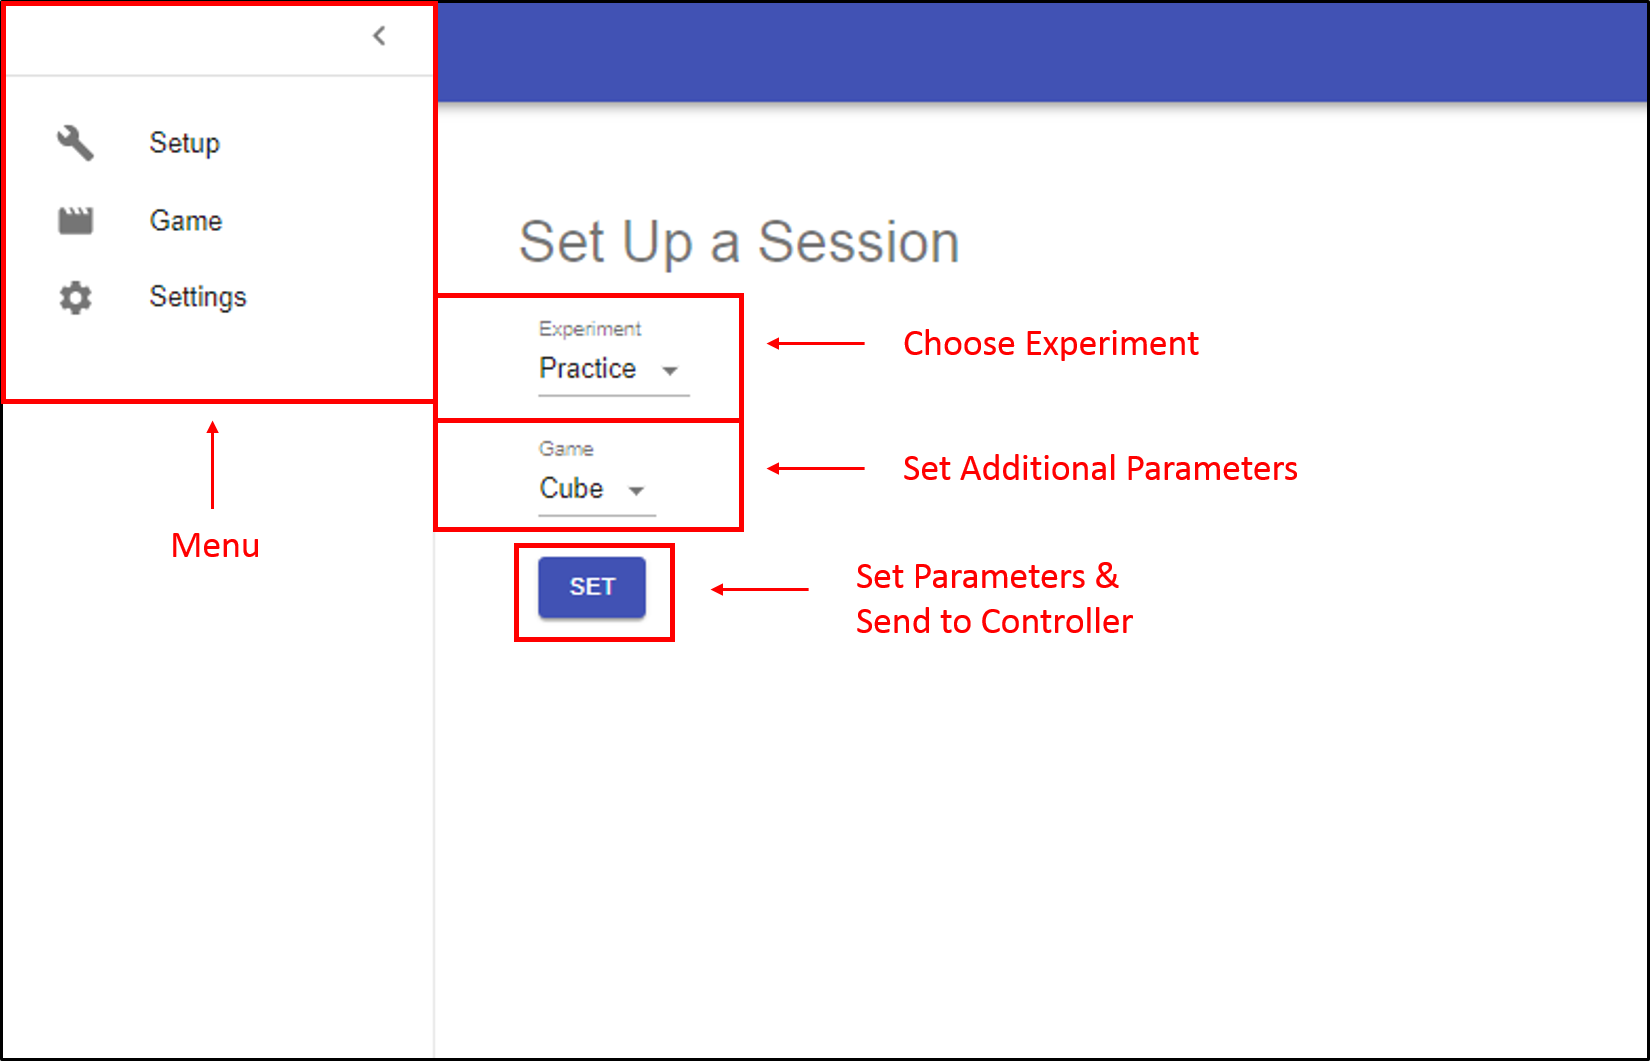
\includegraphics[width=0.9\linewidth]{UI_menu_label}
		\caption{The Setup Page}
		\label{fig:ui-menu}
	\end{figure*} 	
		
\textbf{Games Page}: The game page displays the games or visuals to the patient. It contains the home and run buttons which are used to set up the device before starting the session. 

\textbf{Settings Page}: This page contains any UI settings that one may want to change. For now, this only allows the operator to switch between Developer Mode and User Mode, which change the level of detail in the setup page. 		
		
		\subsubsection{Visuals}
		
		The guide is used to display the length of the actuator, the user's position and the desired position (Fig. \ref{fig:trajectory}). The desired position is shown as a translucent box, which is normally red but changes to green if the user's position is within a certain small margin of error. The User's position is shown as a blue rectangle. In essence, the knee flexion exercise is carried out by the user attempting to follow the desired position as closely as possible. 
		
	\begin{figure*}[h] 
		\centering
		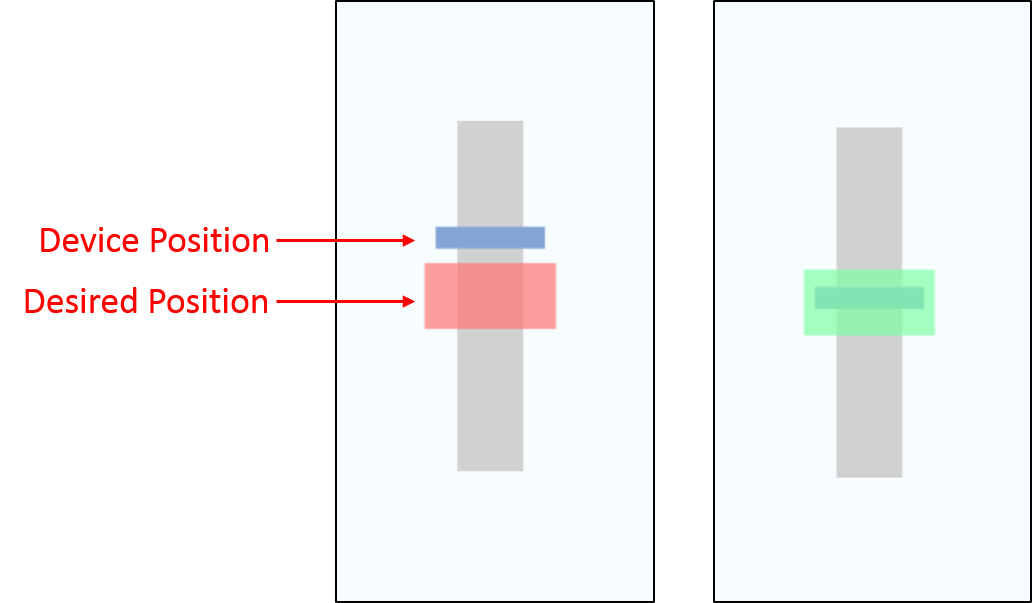
\includegraphics[width=0.75\linewidth]{UI_trajectory}
		\caption{The trajectory guide}
		\label{fig:trajectory}
	\end{figure*} 
	
	Three simple games were created, each corresponding to a different type of game which could be expanded upon by future students. The first is a simple cube, displayed with the guide. If the user is within a certain margin of error, the cube spins, otherwise the cube is still. This is meant to demonstrate a virtual environment which responds to the performance of the user, but is not a competitive or challenging game. 
	
	The second game is a race between three object: the user and two computer controlled characters (Fig. . Each object moves around a track, with the computer characters moving at predefined speeds, and the user's character moving at a speed proportional to the accuracy of their motion (\textit{i.e.} the lower the error, the faster they move). This game is meant to demonstrate a more challenging game which motivates the player to perform the exercise accurately. 

	
	\begin{figure*}[h] 
		\centering
		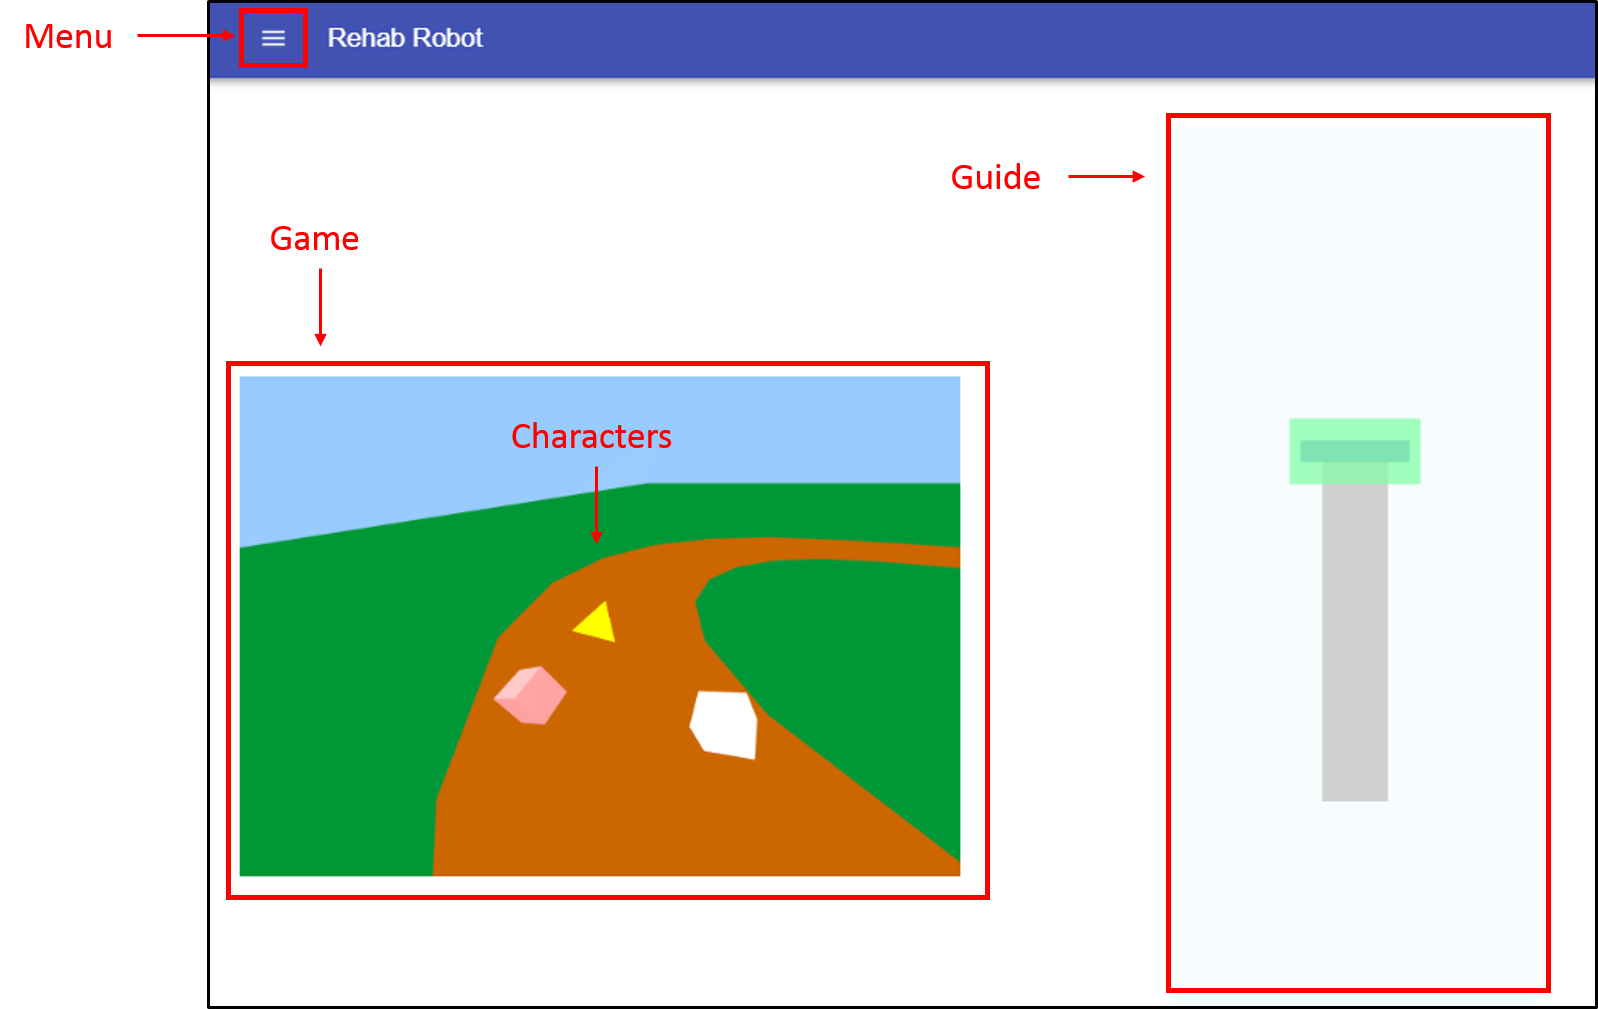
\includegraphics[width=\linewidth]{UI_game_label}
		\caption{The racing game}
		\label{fig:race}
	\end{figure*} 
	

The third game is balancing game which is not related to the knee flexion exercise. The user's foot directly controls the position of their character. They are tasked with maintaining a static position on top of a column (Fig REF). Disturbances are launched at the player in the form of spheres, which when in contact created haptic force feedback according to the physics layed out in Sec. REF. The user must push these disturbances away without falling off the column. This game demonstrates both haptic feedback, and a game in which the user's foot directly control a character. 
			
	\section{Software Extension}
	
			While the software was customized to this system, it is desirable that it can be re-used in future design changes to the device, such as changing the control algorithm, adding DOF's, or changing the UI. To facilitate the use of the software for future designs, the software was re-factored to a more general structure, essentially a software template. The template includes  all initialization steps for creating real-time threads, communication of the UI, and communication with the DAQ -- however the controller and data structures are empty. Instructions are included on adding ...
	
\chapter{Experiments}



	\section{Safety Tests}
	
	The safety features on the device are designed to limit the forces and velocities applied by the robot to the user, and also to prevent over-extending the leg. The safety features to be tested included: 

\textbf{Software Limits}: Software limits are placed on force, velocity, motor command, and position. The motor command is saturated at maximum value. The software limits are tested with some demo code which runs through a variety of trajectories and checks to ensure that the motor command is curtailed as required. ...

\textbf{Motor Current Limit}: The motor controller includes a potentiometer which can set the maximum current running through the motor, effectively limiting the motor torque. This was set to ... This feature is not tested; in the future, a current sensor could be used to verify motor current levels.

\textbf{End stop}: If the leg is pulled straight, or beyond this point, the joint may lock, making any applied force potentially dangerous. An adjustable end stop is used to physically stop the movement of the footplate. The end stop also contains a limit switch so that the system knowns when it has reached the end point. 
...

Other safety features have been included but have not yet been integrated, including hard limits on the motor command. This is done using a comparator to compare the motor command against a fixed voltage level, as described in Sec REF. This features should be fully tested and integrated before testing on patients, who may be in greater danger due to high applied forces. 

	%\begin{enumerate}
	%	\item Software limits on velocity, force, motor command
	%	\item Motor current limits set on the motor controller
	%	\item The adjustable end stop to prevent over extension 
	%\end{enumerate}
	
	\section{Functional Tests}

	\subsection{Verifying Trajectory Generation and Position Control}

	\subsection{Verifying Admittance Control}
	
	The goal of admittance control is to achieve a desired dynamic behaviour, usually in terms of a mass-spring-damper system, given some input force. To confirm that the controller is successfully rendering the desired admittance, the output position of the device was compared to a simulation of the desired admittance. Force was applied to the system, and data regarding the position and the input force was saved. The force data was used as an input to a Simulink simulation of the mass-spring-damper system, and both the robots position and the simulated position were compared. It was expected that the robot position would track the simulation with some minimal delay due to time lag introduced by the finite sampling rate, as well as some possible error due to limitations of the robots PD control. 		

	
\begin{figure*}[t] 
	\centering
	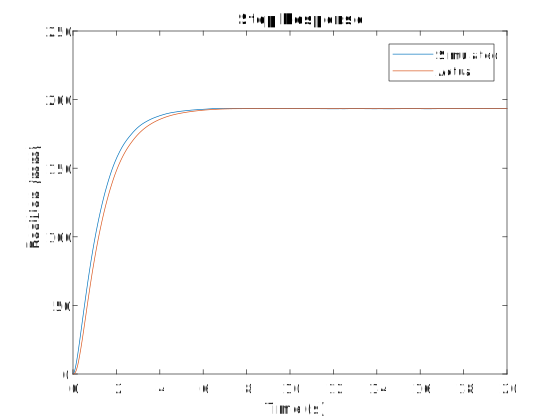
\includegraphics[width=0.9\linewidth]{Mar12_NoForce_Step_Plot}
	\caption{Admittance Verification with Interaction}
	\label{fig:nVerNoInt}
\end{figure*}
	
For the first test no interaction force was applied, only an initial offset of the reference position of the spring (of 0.2m) was used to elicit a response. A comparison of the robot's behaviour and the simulated behaviour of the desired admittance behaviour is given in (Fig. \ref{fig:nVerNoInt}). The system behaved as expected, following the correct admittance with a small delay.

The next test was to apply forces to the system to determine if the system can render the correct admittance with a semi-random input. Hence, a human subject was tasked with moving back and forth. The force data was saved and used as an input to the admittance simulation. Fig. \ref{fig:adm_sim} shows a comparison of the actual device position versus the simulated position. Again, the system behaves as expected, following the simulation with some minimal delay.

\begin{figure}[h]
	\centering
	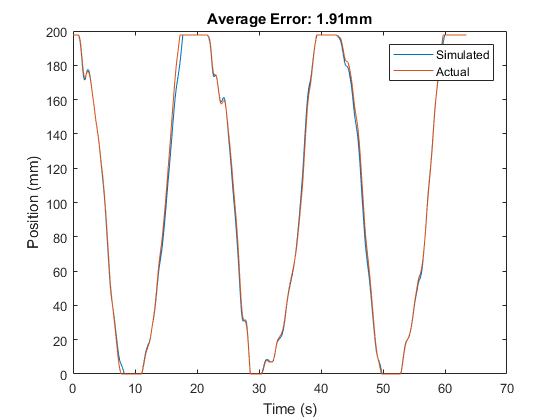
\includegraphics[width=0.9\textwidth]{admittance_sim}
	\caption{Robot admittance position vs simulated position based on force data}
	\label{fig:adm_sim}
\end{figure}	

%\begin{figure}[h]
%	\centering
%	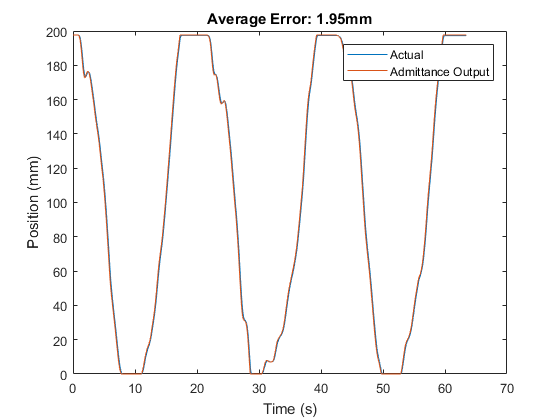
\includegraphics[width=0.9\textwidth]{admittance_v_position}
%	\caption{Robot admittance position vs actual position of device}
%	\label{fig:adm_pos}
%\end{figure}	
	
		
	These tests confirm that the admittance controller adequately recreated the desired dynamics, and that the outer-loop PD controller tracked this behaviour. 
	
	\subsection{Verifying Haptic Control}
	
	Two aspects of the haptic controller were tested. First, the haptic coupling was tested to confirm that it was providing the minimal impedance as described by its mass and damping parameters (REF). This was done by running the controller with the interaction force set to zero. The final result should be equivalent to admittance control without the spring term. ...
	
	Next, the haptic controller's ability to render interaction forces correctly was tested. 
	
	\section{Healthy Subject Experiments}
	
	
	
		\subsection{Method}
		
		Five subjects were recruited to participate in a pilot study under ethics approval from Carleton University's REB. This was a preliminary study and so was done on healthy subjects with motor control over their legs. The purpose of the study was threefold: to test the function and safety of the device, to study the affects of different levels of assistance and resistance, and to get subjective data concerning the device and the three types of games. The experiment consisted of two phases: 

\textbf{Parameter Ranges}: Subjects went through ten 1-minute trials with varying levels of assistance and resistance. Five trials included changing levels of assistance with constant resistance, and the other five had no assistance and changing levels of resistance. The assistance levels varied from 0.1 to 0.6 N/mm (with a constant damping of 0.2 Ns/mm), and then the damping varied from 0.1 to 0.6 Ns/mm. The order of the levels was changed between subjects to prevent time-based biasing due to learning or fatigue. Each trial required the subject to follow a desired trajectory, moving back and forth through the knee extension exercise, each at the same velocity. 

\textbf{Games \& Visual}: The next phase consisted of three 1.5-minute trials covering the three games described in REF. The user played each game and then was asked to comment on their levels of effort, engagement, the difficulty of the task, and the distractibility of the visuals. 

Data collection included data logged from the robot and subjective questionnaire answers. Relevant data from the robot included position, desired position, velocity, and force. From these, error and effort are calculated:

\begin{equation}
\text{error} = \frac{\sum |x - x_{des}|}{N}
\end{equation}
\begin{equation}
\text{effort} = \sum |vF|
\end{equation}

The average error is the sum of the error between the device's position and the desired position. It is hypothesized that higher levels of assistance and lower levels of resistance will lead to lower levels of error. 

The effort captures the power input from the user to the device. It is difficult to distinguish between force reading due to the user applying force to the device, and the device applying force to the user when providing assistance. An approximation was to consider force applied in the correct direction (\textit{i.e.} towards the desired position) as contributing positively to total effort, and force in the wrong direction as negative effort. This is motivated by the fact that if the system is providing assistance, or is driving the motion, than it will be pulling the user's leg in the direction of the desired trajectory, resulting in a force in the opposite direction of the desired point. 
	
\begin{equation}
\text{effort} =  \sum \text{sgn}(err)\text{sgn}(F)|vF|
\end{equation}	

It is hypothesized that total user effort will be lower with higher assistance, and will be much higher with higher levels of resistance. If these metrics (error and effort) correlate well, then they may be of use for therapists to track patient progress. 
	
		\subsection{Result}
		
		The soft real-time system was capable of providing reasonably precise time step control, with an average time step of 1.05 ms (5\% higher than the goal of 1ms). Jitter was higher during some steps, sometimes reaching up to 2ms, however this did not affect the systems ability to deliver the proper controls. 

%	\begin{itemize}
%		\item Time step jitter to determine how well the real time system could achieve the desired frequency 
%		\item Testing how well the actual position of the device matches the position of the admittance simulation
%	\end{itemize}

\begin{figure*}[t] 
	\centering
	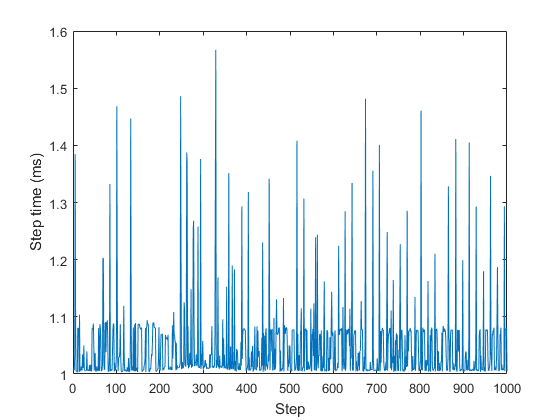
\includegraphics[width=0.9\linewidth]{time_jitter}
	\caption{Time jitter over 1 second of operation}
	\label{fig:jitter}
\end{figure*}

One issue discovered was time lag in the UI visuals. Occasionally the visuals would freeze, for approximately 1 - 2 seconds. This can be annoying for the user and makes following the desired trajectory displayed by the guide. The origin of the time lag is unknown -- it could be issues with the wireless network, or with the websocket communication. Further investigation is required. 

	
	\subsection{Admittance Ranges}
	
	The differing levels of assistance had some impact on the participant's performance. Fig. \ref{fig:pos_comp} gives an example of how the higher levels of assistance can help reduce error. The figure shows the position of the user through a single stroke (back and forth), compared to the desired trajectory in green. At the lower level, the user actually overshoots the trajectory when moving from back to front, whereas at the higher assistance level the overshoot is presumably corrected by assistive forces, allowing the user to follow the trajectory more closely. 
	
	
\begin{figure*}[h] 
	\centering
	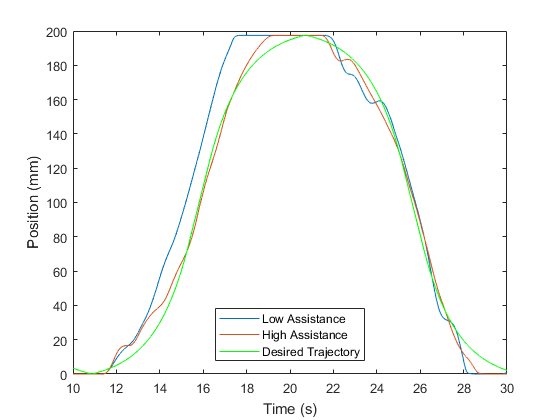
\includegraphics[width=0.75\linewidth]{position_comp}
	\caption{Comparison between high and low assistance levels}
	\label{fig:pos_comp}
\end{figure*}

Both error and effort decrease as assistance levels are increased, as seen in Fig. \ref{fig:err_assist}. The error trend is small compared to the standard deviation, potentially due to the fact that these are healthy subjects who do not necessarily require assistance in achieving the trajectory. The effort trend is more pronounced, indicating that the participants did not need to apply as much effort to achieve the trajectory when assistance levels are high.
	
\begin{figure}[h]
	\centering
	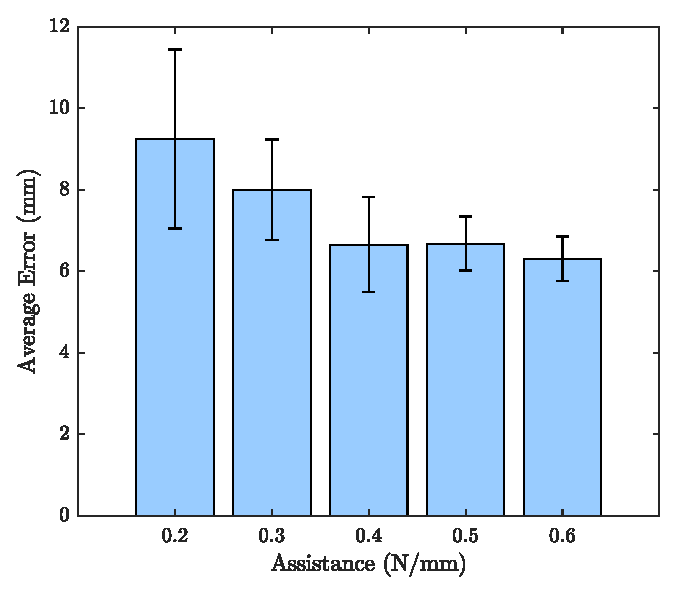
\includegraphics[width=0.45\textwidth]{err_assist}
	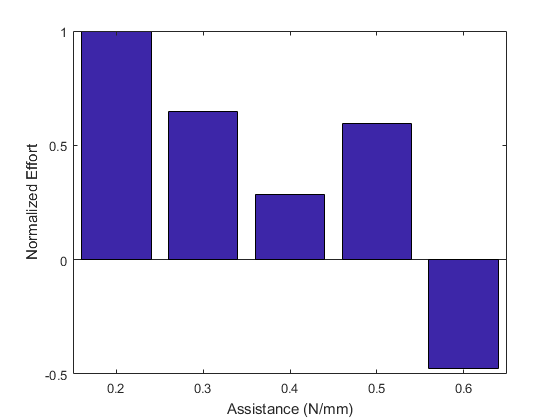
\includegraphics[width=0.45\textwidth]{eff_assist}
	\caption{Mean error from desired position (left) and total effort (right) for different assistance levels}
	\label{fig:err_assist}
\end{figure}	
		
The participants found resistance mode more difficult than assistance mode, as demonstrated by the error and effort metrics. This is in part due to the increased force required to move the device at higher resistance levels. This can be seen when comparing force data, as in Fig. \ref{fig:force_comp}. The user in general applies less force in assistance mode, especially when the device is moving at high speeds. 

\begin{figure*}[h] 
	\centering
	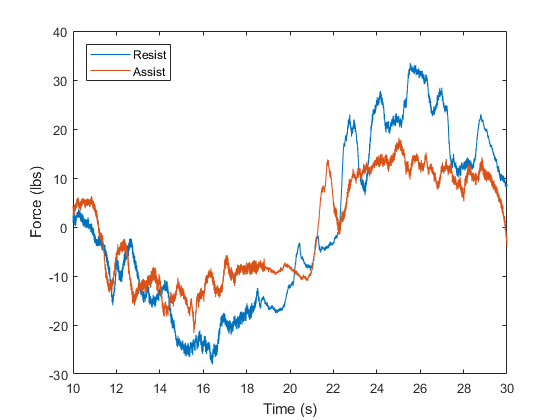
\includegraphics[width=0.75\linewidth]{force_comp}
	\caption{Comparison of forces between assistance and resistance modes}
	\label{fig:force_comp}
\end{figure*}
	
The effects of the resistance level on error and effort are shown in Fig. \ref{fig:err_resist}. The resistance did not have a significant effect on the level of error; there is a spike at 0.3 Ns/mm, although this is probably due to other factors. It seems more likely that gradual changes in resistance do not effect a healthy subject's ability to perform the trajectory. Increasing the resistance level increased user effort, as predicted. This is due to the fact that higher resistance levels by definition require greater force to move at a given velocity, hence increasing the required effort. 

\begin{figure}[h]
	\centering
	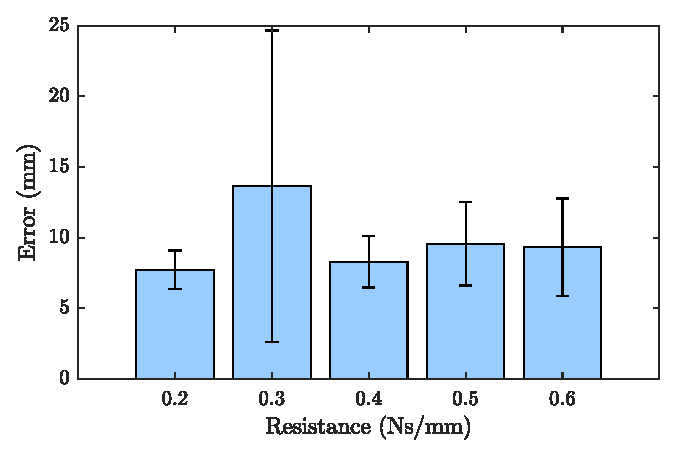
\includegraphics[width=0.45\textwidth]{err_resist}
	\includegraphics[width=0.45\textwidth]{eff_resist}
	\caption{Mean error from desired position (left) and total effort (right) for different resistance levels}
	\label{fig:err_resist}
\end{figure}		


The subjective scores of difficulty are shown in Fig \ref{fig:difficulty}. These scores were normalized to each participant, averaged, and then scaled such that the highest score was a 5/5. The raw data can be found in REF. Subjective difficulty did not change dramatically for different levels of assistance, although the small trend does show that participant's found higher assistance levels less difficult. The small trend is probably due to the fact that the healthy subjects were able to track the trajectory well, and so only received small amounts of assistance. However, as indicated above, the assistance level did have a small impact on error and effort. 

\begin{figure}[h]
	\centering
	\includegraphics[width=0.45\textwidth]{diff_assist}
	\includegraphics[width=0.45\textwidth]{diff_resist}
	\caption{Subjective Difficulty Scores across assistance and resistance levels}
	\label{fig:difficulty}
\end{figure}	

The resistance levels show a different trend, with the medium levels of resistance receiving the lowest difficulty, and the lower and higher levels of resistance each being more difficult. Some user's preferred lower resistance, stating that this allowed for more transparent motion. Others preferred medium to high levels of resistance, because they liked to ``push'' through the motion with greater force, and because they found that they often overshot the desired trajectory when resistance was too low. One user experienced small amounts of instability at the lowest level of resistance (0.1 Ns/mm).  
	
	\subsection{Efficacy of Games}
	
	The participant's ranked the level of engagement, effort, difficulty, and how distracting the visuals were, each on a scale of 1 to 5. The results are shown in Table \ref{tab:games}. On average, the user's preferred the racing game and the balance game. The cube game was not found to be engaging, as indicated by its low score of 1.75/5. The other measures did not vary significantly across games. Both the cube game and the racing game were found to be somewhat distracting (3/5). 	
	
	\begin{table}[h] \label{tab:games}
	\centering
	\begin{tabular}{l c c c c }
	\toprule
	Game & Engagement & Effort & Difficulty & Distractibility \\
	\midrule
	\rowcolor{gray!10} Simple Environment & 1.75 & 2  & 1.75 & 2.9 \\
	Racing Game & 4 & 2.3 & 1.9 & 3 \\
	\rowcolor{gray!10} Haptic Balance & 4.4 & 3.5 & 2.5 & N/A \\
	\bottomrule
	\end{tabular}
	\end{table}	
	
\subsection{General Comments}
	
	The participants ranked several general aspects of the robot on a scale of 1 to 5, including the comfort and safety of the robot, as well as how well the visuals corresponded to the functioning of the robot, and how well it supported their leg.
	
	\begin{table}[h]
	\centering
	\begin{tabular}{l c c c c c c c }
	\toprule
	Subject & 1 & 2 & 3 & 4 & 5 & 6 & Average \\
	\midrule
	\rowcolor{gray!10} Comfort & 3.5 & 5 & 3.5 & 1.5 & 1.5 & 3.5 & 3.2 \\
	Safety & 5 & 5 & 5 & 5 & 4  & 5 & 4.8 \\
	\rowcolor{gray!10} Visual Correspondence & 4 & 5 & 5 & 3 & 5 & 5 & 4.5  \\
	Leg Support & 2 & 2 & 1 & 2 & 1  & 2 & 1.7 \\
	\bottomrule
	\end{tabular}
	\end{table}
	

		
		\subsection{Discussion}
		
		The first goal of the experiment was to test a range of assistance and resistance levels to determine which are suitable and how they influence the user's performance. As shown in Fig. \ref{fig:err_assist} and Fig. \ref{fig:eff_assist}, the increasing the level of assistance leads to on average lower levels of error, and lower net effort applied by the user. This trend holds despite some of the user's reporting that they did not feel a difference between differing levels of assistance. This results indicates that increasing the spring stiffness can be used to better help patient's who may need assistance to follow the trajectory, and who may not be physically capable of applying enough effort. 
		
		The levels of resistance were also correlated with user effort (Fig. \ref{fig:eff_resist}), as greater damping requires the user to apply more force. However, resistance was not correlated with user error (Fig. \ref{fig:err_assist}. This aligns with the particpant's subjective scores, which show that different participants preferred different levels of resistance. Some preferred lower levels, as these allow for easier and more transparent motion. Some preferred higher levels of resistance, as this allows the user to apply force without having to worry about too much overshoot. These results indicate that the resistance level should be tailored to the specific patient, perhaps with some kind of calibration step.  
		
		...
		
		The general questions were used to determine participant's views on the comfort of the device, bed and UI, the percieved safety, the correspondence between the visual guide and the participant's position, and the leg support provided by the footplate. Safety and visual correspondence received  consistent high scores, with an average of 4.8 and 4.5/5, respectively. Visual correspondence was marred only by occasional lag in UI which caused the games to freeze momentarily. The device comfort received mixed reviews, with an average of 3.2/5. The comfort score was an aggregate of the comfort of the UI, the footplate, the bed, and an overall score.... The leg support consistently got low ratings, with an average of 1.7/5. This was due to several factors. First, due to some instabilities in the footplate described in REF. The heel rest was also uncomfortable, which affected this score. ...
		
		\subsection{Other Comments and Advice}

Participants were asked to comment on how they thought the device could be improved. These comments are enumerated here, and will influence the future work section in REF. 		
		
		\begin{enumerate}
			\item Some users found the heel rest uncomfortable. 
			\item The simple visual environment (with the spinning cube) confused some participants.
			\item The motor makes a ringing noise when on, which annoyed some.
		
		\end{enumerate}
		
	
	
\chapter{Conclusion}

	Rehabilitation Robots have been used successfully in both research and clinical settings. Many devices exist, primarily for the upper-limbs and for gait training. The gap in the researcher concerning devices for bed-bound therapy for acute stroke patients motivated the construction of ViGRR. 
	
	
\begin{figure}[h]
	\centering
	\includegraphics[width=0.9\textwidth]{robot_cad}
	\caption{The rehabilitation robot and user interface}
	\label{fig:robot_cad}
\end{figure}		
		

	\section{Future Work}
	
	\subsection{Design Additions}
	
	Participants rated the device's ability to support the leg consistently low, at an average of 1.7/5. This needs to be improved before testing on patient's, who will be more dependent on the device for support. 
	
	\begin{enumerate}
		\item Improve heel rest comfort by adding comfortable material, and by extending the rest to hold more of the foot. 
		\item Improving the support of the footplate by using larger brackets to stabilize the cantilever. 
		\item Improving the footplate-load cell attachment by machining the support brackets from aluminium to eliminate flexibility. 
		\item As suggested by therapists, a second support point on the leg is needed so that the patient's leg does not bend out of plane. A passive multi-DOF support point attached under the knee should be added, which can accommodate a variety of leg sizes and stroke lengths. 
	\end{enumerate}		
	
	A case for the PCB and Load Cell amplifier has been created, however the other electronics are lose. A separate box should be built to contain the motor controller, power supply, DAQ and computer. This box should be portable and easily connected to the robot. This would allow the robot to be easily setup and removed as needed in the hospital. 
	
	A shell needs to be built to protect other's from any sharp edges, and so that the device can be cleaned or sterilized as needed. Some research should be done on what material to use. 
	
	Finally, extra DOF's should be added to accommodate different types of exercises. More research will need to be done concerning the best configuration. 
	
	\subsection{User Interface Additions}
	
	\begin{enumerate}
		\item Improve games and visuals
		\item Determine the origin of the occasional lag and fix
		\item Add to setup page to allow therapist's to customize the parameters
		\item Add data viewing page which could allow therapist's to monitor patient progress
	\end{enumerate}
	
	\subsection{Trials}
	
	
\chapter*{Appendix I: CAD Drawings}
\chapter*{Appendix II: PCB Diagram \& BOM}

		
	\begin{figure*}[t] 
		\centering
		\includegraphics[width=\linewidth]{pcb_schematic}
		\caption{Printed Circuit Board}
		\label{fig:pcb}
	\end{figure*}

	\begin{table}[]
	\centering
	\caption{PCB Components}	
	\begin{tabular}{|l|l|}
		\hline
		\textbf{Component} & \textbf{Description}  \\ \hline
		24 V DC/DC Converter & Converts 48V to 24V  \\ \hline
		10 \& 5V Linear Regulator & Converts 48V to 10V and 5V  \\ \hline
		OP-AMP & Signal Processing   \\ \hline
		Comparator & Checks to ensure commands are not above/below threshold   \\ \hline
		4 Channel AND Gate & Only enables operation if all saftey checks read ok   \\ \hline
		Watchdog Timer & Ensures controller is still running \\ \hline

		\end{tabular}
	\label{tab:belt}
	\end{table}

\chapter*{Appendix III: Hardware Datasheets}

	\begin{figure*}[h] 
		\centering
		\includegraphics[width=0.75\linewidth]{Motor_range}
		\caption{Operating Range of the Motor \newline \small www.maxongroup.com/maxon/view/product/motor/dcmotor/re/re50/370354}
		\label{fig:motor_range}
	\end{figure*}

\chapter*{Appendix IV: Complete Data from Fieldwork at Hospital}


	\setlength\arrayrulewidth{1pt}	
	
	\begin{table}[ht]
	\centering
	\begin{tabular}{c c c c c c}
	\toprule
	Mode & Level & Error & Effort & Overshoot & Difficulty \\
	& & \tiny $[mm]$ & \tiny $[N mm/s]$ & \tiny $[mm]$ & \\
	\midrule
	\cellcolor{white} 						& 1 & 5.00 & 5.00 &  & 2.75 \\ 
	\rowcolor{gray!10}		
	\cellcolor{white}						& 2 & 4.35 & 3.15 & & 2.73 \\ 
	\cellcolor{white}						& 3 & 3.55 & 2.60 & & 1.95 \\ 
	\rowcolor{gray!10}
	\cellcolor{white}						& 4 & 3.52 & 2.13 & & 2.24 \\ 
	\cellcolor{white}	\multirow{-5}{*}{Assist} 	& 5 & 3.40  & 1.84 & & 2.23 \\ 
	\midrule
	\rowcolor{gray!10}
	\cellcolor{white} 						& 1 & 4.07 & 2.15 & & 3.50 \\ 
	\cellcolor{white}
	\cellcolor{white}						& 2 & 10.40 & 2.76 & & 2.01 \\
	\rowcolor{gray!10}
	\cellcolor{white}						& 3 & 4.98 & 5.11 & & 2.61 \\ 
	\cellcolor{white}						& 4 & 6.10 & 4.44 & & 4.37 \\ 
	\rowcolor{gray!10}
	\cellcolor{white}	\multirow{-5}{*}{Resist}		& 5 & 5.61 & 7.34 & & 5.00 \\ 
	\bottomrule
	\end{tabular}
	\end{table}
	
	
\bibliography{thesis}
\bibliographystyle{ieeetr}
\end{document}